% Options for packages loaded elsewhere
\PassOptionsToPackage{unicode}{hyperref}
\PassOptionsToPackage{hyphens}{url}
\documentclass[
]{article}
\usepackage{xcolor}
\usepackage[margin=1in]{geometry}
\usepackage{amsmath,amssymb}
\setcounter{secnumdepth}{-\maxdimen} % remove section numbering
\usepackage{iftex}
\ifPDFTeX
  \usepackage[T1]{fontenc}
  \usepackage[utf8]{inputenc}
  \usepackage{textcomp} % provide euro and other symbols
\else % if luatex or xetex
  \usepackage{unicode-math} % this also loads fontspec
  \defaultfontfeatures{Scale=MatchLowercase}
  \defaultfontfeatures[\rmfamily]{Ligatures=TeX,Scale=1}
\fi
\usepackage{lmodern}
\ifPDFTeX\else
  % xetex/luatex font selection
\fi
% Use upquote if available, for straight quotes in verbatim environments
\IfFileExists{upquote.sty}{\usepackage{upquote}}{}
\IfFileExists{microtype.sty}{% use microtype if available
  \usepackage[]{microtype}
  \UseMicrotypeSet[protrusion]{basicmath} % disable protrusion for tt fonts
}{}
\makeatletter
\@ifundefined{KOMAClassName}{% if non-KOMA class
  \IfFileExists{parskip.sty}{%
    \usepackage{parskip}
  }{% else
    \setlength{\parindent}{0pt}
    \setlength{\parskip}{6pt plus 2pt minus 1pt}}
}{% if KOMA class
  \KOMAoptions{parskip=half}}
\makeatother
\usepackage{graphicx}
\makeatletter
\newsavebox\pandoc@box
\newcommand*\pandocbounded[1]{% scales image to fit in text height/width
  \sbox\pandoc@box{#1}%
  \Gscale@div\@tempa{\textheight}{\dimexpr\ht\pandoc@box+\dp\pandoc@box\relax}%
  \Gscale@div\@tempb{\linewidth}{\wd\pandoc@box}%
  \ifdim\@tempb\p@<\@tempa\p@\let\@tempa\@tempb\fi% select the smaller of both
  \ifdim\@tempa\p@<\p@\scalebox{\@tempa}{\usebox\pandoc@box}%
  \else\usebox{\pandoc@box}%
  \fi%
}
% Set default figure placement to htbp
\def\fps@figure{htbp}
\makeatother
\setlength{\emergencystretch}{3em} % prevent overfull lines
\providecommand{\tightlist}{%
  \setlength{\itemsep}{0pt}\setlength{\parskip}{0pt}}
\usepackage{multirow}
\usepackage{multicol}
\usepackage{colortbl}
\usepackage{hhline}
\newlength\Oldarrayrulewidth
\newlength\Oldtabcolsep
\usepackage{longtable}
\usepackage{array}
\usepackage{hyperref}
\usepackage{float}
\usepackage{wrapfig}
\usepackage{booktabs}
\usepackage{caption}
\usepackage{anyfontsize}
\usepackage{bookmark}
\IfFileExists{xurl.sty}{\usepackage{xurl}}{} % add URL line breaks if available
\urlstyle{same}
\hypersetup{
  pdftitle={Results\_3},
  pdfauthor={Ananya Mazumder},
  hidelinks,
  pdfcreator={LaTeX via pandoc}}

\title{Results\_3}
\author{Ananya Mazumder}
\date{2026-02-05}

\begin{document}
\maketitle

Table for IGMSY districts

Next comes the balance table:

next come the descriptive tables with household and individual level
controls

\begin{table}[t]
\caption{\label{tab:First descriptive table}\textbf{Table 2. Survey-Weighted Descriptives for Women \& Household}} 
\fontsize{12.0pt}{14.0pt}\selectfont
\begin{tabular*}{\linewidth}{@{\extracolsep{\fill}}lcccc}
\toprule
\textbf{Characteristic} & \textbf{Control District × Ineligible}  N = 9786\textsuperscript{\textit{1}} & \textbf{Treated District × Ineligible}  N = 16307\textsuperscript{\textit{1}} & \textbf{Control District × Eligible}  N = 649\textsuperscript{\textit{1}} & \textbf{Treated District × Eligible}  N = 915\textsuperscript{\textit{1}} \\ 
\midrule\addlinespace[2.5pt]
respondent's current age & 37.724
(5.017) & 29.949
(5.216) & 38.887
(4.377) & 32.005
(4.951) \\ 
Square of Women's Age & 1,448.275
(385.819) & 924.133
(333.653) & 1,531.333
(344.042) & 1,048.804
(331.550) \\ 
education in single years & 5.309
(5.071) & 7.082
(5.231) & 7.840
(5.346) & 9.296
(4.946) \\ 
Weight (kg) & 54.164
(11.100) & 51.693
(10.677) & 62.471
(12.867) & 58.748
(11.971) \\ 
Height (cm) & 151.724
(6.192) & 151.627
(6.375) & 153.765
(5.724) & 153.872
(5.860) \\ 
age at first cohabitation & 17.936
(3.831) & 18.773
(3.689) & 19.676
(3.653) & 20.696
(3.842) \\ 
husband/partner drinks alcohol & 388 (31\%) & 533 (28\%) & 20 (35\%) & 25 (26\%) \\ 
total children ever born & 2.953
(1.379) & 2.547
(1.284) & 2.635
(1.094) & 2.312
(1.005) \\ 
husband/partner's total number of years of education & 7.137
(4.943) & 8.025
(5.022) & 7.579
(4.344) & 10.206
(4.363) \\ 
respondent currently working & 513 (34\%) & 537 (23\%) & 20 (26\%) & 20 (19\%) \\ 
ethnicity &  &  &  &  \\ 
    caste & 8,148 (85\%) & 13,158 (84\%) & 484 (98\%) & 704 (97\%) \\ 
    tribe & 923 (9.6\%) & 1,537 (9.8\%) & 3 (0.5\%) & 6 (0.9\%) \\ 
    no caste / tribe & 481 (5.0\%) & 784 (5.0\%) & 3 (0.7\%) & 9 (1.3\%) \\ 
    don't know & 74 (0.8\%) & 175 (1.1\%) & 2 (0.3\%) & 4 (0.6\%) \\ 
number of household members (listed) & 5.275
(2.269) & 5.920
(2.531) & 5.354
(1.940) & 5.926
(2.227) \\ 
number of children 5 and under in household (de jure) &  &  &  &  \\ 
    0 & 8,834 (92\%) & 4,514 (29\%) & 453 (92\%) & 279 (38\%) \\ 
    1 & 554 (5.8\%) & 6,562 (42\%) & 29 (6.0\%) & 305 (42\%) \\ 
    2 & 182 (1.9\%) & 3,691 (24\%) & 8 (1.6\%) & 123 (17\%) \\ 
    3 & 45 (0.5\%) & 675 (4.3\%) & 2 (0.3\%) & 16 (2.3\%) \\ 
    4 & 7 (<0.1\%) & 139 (0.9\%) & 0 (0\%) & 1 (0.2\%) \\ 
    5 & 3 (<0.1\%) & 60 (0.4\%) & 0 (0\%) & 0 (0\%) \\ 
    6 & 0 (0\%) & 13 (<0.1\%) & 0 (0\%) & 0 (0\%) \\ 
sex of household head &  &  &  &  \\ 
    1 & 8,014 (83\%) & 13,128 (84\%) & 413 (84\%) & 623 (86\%) \\ 
    2 & 1,612 (17\%) & 2,527 (16\%) & 79 (16\%) & 101 (14\%) \\ 
age of household head & 47.072
(11.708) & 45.545
(14.770) & 49.292
(12.385) & 49.113
(15.511) \\ 
household has: electricity &  &  &  &  \\ 
    0 & 273 (2.8\%) & 554 (3.5\%) & 0 (<0.1\%) & 1 (0.2\%) \\ 
    1 & 9,258 (96\%) & 14,566 (93\%) & 485 (99\%) & 704 (97\%) \\ 
    7 & 95 (1.0\%) & 535 (3.4\%) & 7 (1.4\%) & 18 (2.5\%) \\ 
household has: radio &  &  &  &  \\ 
    0 & 9,165 (95\%) & 14,552 (93\%) & 460 (94\%) & 659 (91\%) \\ 
    1 & 366 (3.8\%) & 568 (3.6\%) & 25 (5.0\%) & 46 (6.4\%) \\ 
    7 & 95 (1.0\%) & 535 (3.4\%) & 7 (1.4\%) & 18 (2.5\%) \\ 
household has: television &  &  &  &  \\ 
    0 & 3,167 (33\%) & 5,670 (36\%) & 30 (6.1\%) & 54 (7.4\%) \\ 
    1 & 6,364 (66\%) & 9,450 (60\%) & 455 (92\%) & 652 (90\%) \\ 
    7 & 95 (1.0\%) & 535 (3.4\%) & 7 (1.4\%) & 18 (2.5\%) \\ 
household has: refrigerator &  &  &  &  \\ 
    0 & 6,281 (65\%) & 10,171 (65\%) & 66 (13\%) & 107 (15\%) \\ 
    1 & 3,250 (34\%) & 4,949 (32\%) & 419 (85\%) & 599 (83\%) \\ 
    7 & 95 (1.0\%) & 535 (3.4\%) & 7 (1.4\%) & 18 (2.5\%) \\ 
household has: bicycle &  &  &  &  \\ 
    0 & 3,424 (36\%) & 6,903 (44\%) & 192 (39\%) & 274 (38\%) \\ 
    1 & 6,107 (63\%) & 8,217 (52\%) & 293 (59\%) & 432 (60\%) \\ 
    7 & 95 (1.0\%) & 535 (3.4\%) & 7 (1.4\%) & 18 (2.5\%) \\ 
household has: motorcycle/scooter &  &  &  &  \\ 
    0 & 4,914 (51\%) & 7,493 (48\%) & 147 (30\%) & 187 (26\%) \\ 
    1 & 4,617 (48\%) & 7,627 (49\%) & 337 (69\%) & 519 (72\%) \\ 
    7 & 95 (1.0\%) & 535 (3.4\%) & 7 (1.4\%) & 18 (2.5\%) \\ 
household has: car/truck &  &  &  &  \\ 
    0 & 8,810 (92\%) & 13,888 (89\%) & 377 (77\%) & 554 (77\%) \\ 
    1 & 721 (7.5\%) & 1,232 (7.9\%) & 108 (22\%) & 151 (21\%) \\ 
    7 & 95 (1.0\%) & 535 (3.4\%) & 7 (1.4\%) & 18 (2.5\%) \\ 
wealth index combined &  &  &  &  \\ 
    1 & 283 (26\%) & 438 (26\%) & 1 (1.9\%) & 1 (1.1\%) \\ 
    2 & 228 (21\%) & 324 (19\%) & 4 (9.1\%) & 3 (3.9\%) \\ 
    3 & 192 (18\%) & 310 (18\%) & 6 (13\%) & 8 (10\%) \\ 
    4 & 179 (17\%) & 328 (19\%) & 8 (18\%) & 13 (17\%) \\ 
    5 & 201 (19\%) & 306 (18\%) & 26 (58\%) & 53 (68\%) \\ 
wealth index within state &  &  &  &  \\ 
    1 & 276 (25\%) & 419 (25\%) & 8 (18\%) & 8 (11\%) \\ 
    2 & 216 (20\%) & 343 (20\%) & 9 (19\%) & 8 (10\%) \\ 
    3 & 228 (21\%) & 350 (21\%) & 12 (27\%) & 21 (27\%) \\ 
    4 & 185 (17\%) & 288 (17\%) & 9 (21\%) & 21 (27\%) \\ 
    5 & 179 (17\%) & 306 (18\%) & 7 (16\%) & 19 (25\%) \\ 
\bottomrule
\end{tabular*}
\begin{minipage}{\linewidth}
\textsuperscript{\textit{1}}Mean (SD) for continuous variables; N (\%) for categorical variables. N represents unweighted sample size.Wealth indices: 1 = Poorest, 5 = Richest. Sex of HH head: 1 = Male, 2 = Female. Binary variables: 0 = No, 1 = Yes, 7 = Not a dejure resident (where applicable). For all indicators based on the household members (PR file), either the de jure population (usual resident of the house) or the de facto population (slept at the home last night) is selected.\\
\end{minipage}
\end{table}

the next is a descriptive table for men, and their characteristics.

\begin{table}[t]
\caption{\label{tab:Second descriptive-table}\textbf{Table 3. Survey-Weighted Descriptives for Men}} 
\fontsize{12.0pt}{14.0pt}\selectfont
\begin{tabular*}{\linewidth}{@{\extracolsep{\fill}}lcccc}
\toprule
\textbf{Characteristic} & \textbf{Control District × Ineligible}  N = 9786\textsuperscript{\textit{1}} & \textbf{Treated District × Ineligible}  N = 16307\textsuperscript{\textit{1}} & \textbf{Control District × Eligible}  N = 649\textsuperscript{\textit{1}} & \textbf{Treated District × Eligible}  N = 915\textsuperscript{\textit{1}} \\ 
\midrule\addlinespace[2.5pt]
number of wives/partners &  &  &  &  \\ 
    0 & 2 (0.2\%) & 3 (0.2\%) & 0 (0\%) & 0 (0\%) \\ 
    1 & 1,239 (99\%) & 1,985 (100\%) & 26 (100\%) & 44 (100\%) \\ 
    2 & 12 (1.0\%) & 7 (0.3\%) & 0 (0\%) & 0 (0\%) \\ 
total number of years of education & 6.872
(4.785) & 8.004
(4.976) & 7.942
(3.812) & 10.146
(4.086) \\ 
age of respondent at 1st birth & 25.104
(4.878) & 26.171
(4.915) & 24.800
(4.712) & 26.958
(5.059) \\ 
wealth index for urban/rural &  &  &  &  \\ 
    1 & 350 (28\%) & 498 (25\%) & 0 (0\%) & 1 (1.7\%) \\ 
    2 & 247 (20\%) & 455 (23\%) & 1 (2.0\%) & 2 (4.4\%) \\ 
    3 & 225 (18\%) & 340 (17\%) & 6 (22\%) & 3 (7.8\%) \\ 
    4 & 233 (19\%) & 381 (19\%) & 6 (24\%) & 12 (28\%) \\ 
    5 & 199 (16\%) & 321 (16\%) & 13 (52\%) & 26 (58\%) \\ 
wealth index within state &  &  &  &  \\ 
    1 & 328 (26\%) & 449 (23\%) & 5 (17\%) & 4 (10\%) \\ 
    2 & 238 (19\%) & 421 (21\%) & 5 (21\%) & 5 (12\%) \\ 
    3 & 277 (22\%) & 437 (22\%) & 6 (25\%) & 12 (27\%) \\ 
    4 & 225 (18\%) & 344 (17\%) & 6 (22\%) & 11 (26\%) \\ 
    5 & 186 (15\%) & 344 (17\%) & 4 (15\%) & 11 (25\%) \\ 
currently working & 1,132 (90\%) & 1,839 (92\%) & 25 (96\%) & 40 (91\%) \\ 
\bottomrule
\end{tabular*}
\begin{minipage}{\linewidth}
\textsuperscript{\textit{1}}Mean (SD) for continuous variables; N (\%) for categorical variables. 0 = no, 1 = yes for binary variables. Wealth indices: 1 = Poorest, 5 = Richest.\\
\end{minipage}
\end{table}

The table above displays certain characteristics of men in the sample.
These men are married, and matched to women in the sample. DO we know
why some men are unmarried??

\global\setlength{\Oldarrayrulewidth}{\arrayrulewidth}

\global\setlength{\Oldtabcolsep}{\tabcolsep}

\setlength{\tabcolsep}{2pt}

\renewcommand*{\arraystretch}{1.5}



\providecommand{\ascline}[3]{\noalign{\global\arrayrulewidth #1}\arrayrulecolor[HTML]{#2}\cline{#3}}

\begin{longtable}[c]{|p{2.54in}|p{1.24in}|p{0.82in}|p{1.24in}|p{0.82in}|p{1.24in}|p{0.82in}|p{1.24in}|p{0.82in}|p{1.24in}|p{0.82in}|p{1.24in}|p{0.82in}|p{1.24in}|p{0.82in}}

\caption{Survey-Weighted\ DiD\ Results:\ Women's\ Decision-making,\ No\ Controls}\\

\ascline{1pt}{000000}{1-15}

\multicolumn{1}{>{\raggedright}m{\dimexpr 2.54in+0\tabcolsep}}{\textcolor[HTML]{000000}{\fontsize{11}{11}\selectfont{\ }}} & \multicolumn{2}{>{\centering}m{\dimexpr 2.06in+2\tabcolsep}}{\textcolor[HTML]{000000}{\fontsize{11}{11}\selectfont{Own\ Earnings}}} & \multicolumn{2}{>{\centering}m{\dimexpr 2.06in+2\tabcolsep}}{\textcolor[HTML]{000000}{\fontsize{11}{11}\selectfont{Own\ Healthcare}}} & \multicolumn{2}{>{\centering}m{\dimexpr 2.06in+2\tabcolsep}}{\textcolor[HTML]{000000}{\fontsize{11}{11}\selectfont{Large\ Purchases}}} & \multicolumn{2}{>{\centering}m{\dimexpr 2.06in+2\tabcolsep}}{\textcolor[HTML]{000000}{\fontsize{11}{11}\selectfont{Visiting\ Family}}} & \multicolumn{2}{>{\centering}m{\dimexpr 2.06in+2\tabcolsep}}{\textcolor[HTML]{000000}{\fontsize{11}{11}\selectfont{Husband's\ Money}}} & \multicolumn{2}{>{\centering}m{\dimexpr 2.06in+2\tabcolsep}}{\textcolor[HTML]{000000}{\fontsize{11}{11}\selectfont{Autonomy\ Index}}} & \multicolumn{2}{>{\centering}m{\dimexpr 2.06in+2\tabcolsep}}{\textcolor[HTML]{000000}{\fontsize{11}{11}\selectfont{Autonomy\ Dummy}}} \\

\ascline{1pt}{000000}{1-15}



\multicolumn{1}{>{\raggedright}m{\dimexpr 2.54in+0\tabcolsep}}{\textcolor[HTML]{000000}{\fontsize{11}{11}\selectfont{\textbf{Characteristic}}}\textcolor[HTML]{000000}{\fontsize{11}{11}\selectfont{\textsuperscript{1}}}} & \multicolumn{1}{>{\centering}m{\dimexpr 1.24in+0\tabcolsep}}{\textcolor[HTML]{000000}{\fontsize{11}{11}\selectfont{\textbf{Beta}}}\textcolor[HTML]{000000}{\fontsize{11}{11}\selectfont{\textsuperscript{1}}}} & \multicolumn{1}{>{\centering}m{\dimexpr 0.82in+0\tabcolsep}}{\textcolor[HTML]{000000}{\fontsize{11}{11}\selectfont{\textbf{p-value}}}\textcolor[HTML]{000000}{\fontsize{11}{11}\selectfont{\textsuperscript{1}}}} & \multicolumn{1}{>{\centering}m{\dimexpr 1.24in+0\tabcolsep}}{\textcolor[HTML]{000000}{\fontsize{11}{11}\selectfont{\textbf{Beta}}}\textcolor[HTML]{000000}{\fontsize{11}{11}\selectfont{\textsuperscript{1}}}} & \multicolumn{1}{>{\centering}m{\dimexpr 0.82in+0\tabcolsep}}{\textcolor[HTML]{000000}{\fontsize{11}{11}\selectfont{\textbf{p-value}}}\textcolor[HTML]{000000}{\fontsize{11}{11}\selectfont{\textsuperscript{1}}}} & \multicolumn{1}{>{\centering}m{\dimexpr 1.24in+0\tabcolsep}}{\textcolor[HTML]{000000}{\fontsize{11}{11}\selectfont{\textbf{Beta}}}\textcolor[HTML]{000000}{\fontsize{11}{11}\selectfont{\textsuperscript{1}}}} & \multicolumn{1}{>{\centering}m{\dimexpr 0.82in+0\tabcolsep}}{\textcolor[HTML]{000000}{\fontsize{11}{11}\selectfont{\textbf{p-value}}}\textcolor[HTML]{000000}{\fontsize{11}{11}\selectfont{\textsuperscript{1}}}} & \multicolumn{1}{>{\centering}m{\dimexpr 1.24in+0\tabcolsep}}{\textcolor[HTML]{000000}{\fontsize{11}{11}\selectfont{\textbf{Beta}}}\textcolor[HTML]{000000}{\fontsize{11}{11}\selectfont{\textsuperscript{1}}}} & \multicolumn{1}{>{\centering}m{\dimexpr 0.82in+0\tabcolsep}}{\textcolor[HTML]{000000}{\fontsize{11}{11}\selectfont{\textbf{p-value}}}\textcolor[HTML]{000000}{\fontsize{11}{11}\selectfont{\textsuperscript{1}}}} & \multicolumn{1}{>{\centering}m{\dimexpr 1.24in+0\tabcolsep}}{\textcolor[HTML]{000000}{\fontsize{11}{11}\selectfont{\textbf{Beta}}}\textcolor[HTML]{000000}{\fontsize{11}{11}\selectfont{\textsuperscript{1}}}} & \multicolumn{1}{>{\centering}m{\dimexpr 0.82in+0\tabcolsep}}{\textcolor[HTML]{000000}{\fontsize{11}{11}\selectfont{\textbf{p-value}}}\textcolor[HTML]{000000}{\fontsize{11}{11}\selectfont{\textsuperscript{1}}}} & \multicolumn{1}{>{\centering}m{\dimexpr 1.24in+0\tabcolsep}}{\textcolor[HTML]{000000}{\fontsize{11}{11}\selectfont{\textbf{Beta}}}\textcolor[HTML]{000000}{\fontsize{11}{11}\selectfont{\textsuperscript{1}}}} & \multicolumn{1}{>{\centering}m{\dimexpr 0.82in+0\tabcolsep}}{\textcolor[HTML]{000000}{\fontsize{11}{11}\selectfont{\textbf{p-value}}}\textcolor[HTML]{000000}{\fontsize{11}{11}\selectfont{\textsuperscript{1}}}} & \multicolumn{1}{>{\centering}m{\dimexpr 1.24in+0\tabcolsep}}{\textcolor[HTML]{000000}{\fontsize{11}{11}\selectfont{\textbf{Beta}}}\textcolor[HTML]{000000}{\fontsize{11}{11}\selectfont{\textsuperscript{1}}}} & \multicolumn{1}{>{\centering}m{\dimexpr 0.82in+0\tabcolsep}}{\textcolor[HTML]{000000}{\fontsize{11}{11}\selectfont{\textbf{p-value}}}\textcolor[HTML]{000000}{\fontsize{11}{11}\selectfont{\textsuperscript{1}}}} \\

\ascline{1pt}{000000}{1-15}\endfirsthead \caption[]{Survey-Weighted\ DiD\ Results:\ Women's\ Decision-making,\ No\ Controls}\\

\ascline{1pt}{000000}{1-15}

\multicolumn{1}{>{\raggedright}m{\dimexpr 2.54in+0\tabcolsep}}{\textcolor[HTML]{000000}{\fontsize{11}{11}\selectfont{\ }}} & \multicolumn{2}{>{\centering}m{\dimexpr 2.06in+2\tabcolsep}}{\textcolor[HTML]{000000}{\fontsize{11}{11}\selectfont{Own\ Earnings}}} & \multicolumn{2}{>{\centering}m{\dimexpr 2.06in+2\tabcolsep}}{\textcolor[HTML]{000000}{\fontsize{11}{11}\selectfont{Own\ Healthcare}}} & \multicolumn{2}{>{\centering}m{\dimexpr 2.06in+2\tabcolsep}}{\textcolor[HTML]{000000}{\fontsize{11}{11}\selectfont{Large\ Purchases}}} & \multicolumn{2}{>{\centering}m{\dimexpr 2.06in+2\tabcolsep}}{\textcolor[HTML]{000000}{\fontsize{11}{11}\selectfont{Visiting\ Family}}} & \multicolumn{2}{>{\centering}m{\dimexpr 2.06in+2\tabcolsep}}{\textcolor[HTML]{000000}{\fontsize{11}{11}\selectfont{Husband's\ Money}}} & \multicolumn{2}{>{\centering}m{\dimexpr 2.06in+2\tabcolsep}}{\textcolor[HTML]{000000}{\fontsize{11}{11}\selectfont{Autonomy\ Index}}} & \multicolumn{2}{>{\centering}m{\dimexpr 2.06in+2\tabcolsep}}{\textcolor[HTML]{000000}{\fontsize{11}{11}\selectfont{Autonomy\ Dummy}}} \\

\ascline{1pt}{000000}{1-15}



\multicolumn{1}{>{\raggedright}m{\dimexpr 2.54in+0\tabcolsep}}{\textcolor[HTML]{000000}{\fontsize{11}{11}\selectfont{\textbf{Characteristic}}}\textcolor[HTML]{000000}{\fontsize{11}{11}\selectfont{\textsuperscript{1}}}} & \multicolumn{1}{>{\centering}m{\dimexpr 1.24in+0\tabcolsep}}{\textcolor[HTML]{000000}{\fontsize{11}{11}\selectfont{\textbf{Beta}}}\textcolor[HTML]{000000}{\fontsize{11}{11}\selectfont{\textsuperscript{1}}}} & \multicolumn{1}{>{\centering}m{\dimexpr 0.82in+0\tabcolsep}}{\textcolor[HTML]{000000}{\fontsize{11}{11}\selectfont{\textbf{p-value}}}\textcolor[HTML]{000000}{\fontsize{11}{11}\selectfont{\textsuperscript{1}}}} & \multicolumn{1}{>{\centering}m{\dimexpr 1.24in+0\tabcolsep}}{\textcolor[HTML]{000000}{\fontsize{11}{11}\selectfont{\textbf{Beta}}}\textcolor[HTML]{000000}{\fontsize{11}{11}\selectfont{\textsuperscript{1}}}} & \multicolumn{1}{>{\centering}m{\dimexpr 0.82in+0\tabcolsep}}{\textcolor[HTML]{000000}{\fontsize{11}{11}\selectfont{\textbf{p-value}}}\textcolor[HTML]{000000}{\fontsize{11}{11}\selectfont{\textsuperscript{1}}}} & \multicolumn{1}{>{\centering}m{\dimexpr 1.24in+0\tabcolsep}}{\textcolor[HTML]{000000}{\fontsize{11}{11}\selectfont{\textbf{Beta}}}\textcolor[HTML]{000000}{\fontsize{11}{11}\selectfont{\textsuperscript{1}}}} & \multicolumn{1}{>{\centering}m{\dimexpr 0.82in+0\tabcolsep}}{\textcolor[HTML]{000000}{\fontsize{11}{11}\selectfont{\textbf{p-value}}}\textcolor[HTML]{000000}{\fontsize{11}{11}\selectfont{\textsuperscript{1}}}} & \multicolumn{1}{>{\centering}m{\dimexpr 1.24in+0\tabcolsep}}{\textcolor[HTML]{000000}{\fontsize{11}{11}\selectfont{\textbf{Beta}}}\textcolor[HTML]{000000}{\fontsize{11}{11}\selectfont{\textsuperscript{1}}}} & \multicolumn{1}{>{\centering}m{\dimexpr 0.82in+0\tabcolsep}}{\textcolor[HTML]{000000}{\fontsize{11}{11}\selectfont{\textbf{p-value}}}\textcolor[HTML]{000000}{\fontsize{11}{11}\selectfont{\textsuperscript{1}}}} & \multicolumn{1}{>{\centering}m{\dimexpr 1.24in+0\tabcolsep}}{\textcolor[HTML]{000000}{\fontsize{11}{11}\selectfont{\textbf{Beta}}}\textcolor[HTML]{000000}{\fontsize{11}{11}\selectfont{\textsuperscript{1}}}} & \multicolumn{1}{>{\centering}m{\dimexpr 0.82in+0\tabcolsep}}{\textcolor[HTML]{000000}{\fontsize{11}{11}\selectfont{\textbf{p-value}}}\textcolor[HTML]{000000}{\fontsize{11}{11}\selectfont{\textsuperscript{1}}}} & \multicolumn{1}{>{\centering}m{\dimexpr 1.24in+0\tabcolsep}}{\textcolor[HTML]{000000}{\fontsize{11}{11}\selectfont{\textbf{Beta}}}\textcolor[HTML]{000000}{\fontsize{11}{11}\selectfont{\textsuperscript{1}}}} & \multicolumn{1}{>{\centering}m{\dimexpr 0.82in+0\tabcolsep}}{\textcolor[HTML]{000000}{\fontsize{11}{11}\selectfont{\textbf{p-value}}}\textcolor[HTML]{000000}{\fontsize{11}{11}\selectfont{\textsuperscript{1}}}} & \multicolumn{1}{>{\centering}m{\dimexpr 1.24in+0\tabcolsep}}{\textcolor[HTML]{000000}{\fontsize{11}{11}\selectfont{\textbf{Beta}}}\textcolor[HTML]{000000}{\fontsize{11}{11}\selectfont{\textsuperscript{1}}}} & \multicolumn{1}{>{\centering}m{\dimexpr 0.82in+0\tabcolsep}}{\textcolor[HTML]{000000}{\fontsize{11}{11}\selectfont{\textbf{p-value}}}\textcolor[HTML]{000000}{\fontsize{11}{11}\selectfont{\textsuperscript{1}}}} \\

\ascline{1pt}{000000}{1-15}\endhead



\multicolumn{15}{>{\raggedright}m{\dimexpr 16.99in+28\tabcolsep}}{\textcolor[HTML]{000000}{\fontsize{11}{11}\selectfont{\textsuperscript{1}}}\textcolor[HTML]{000000}{\fontsize{11}{11}\selectfont{Coefficients\ with\ standard\ errors\ (clustered\ at\ district\ level)\ in\ parentheses.\ The\ interaction\ term\ 'eligibility\_status\ ×\ treated\_district'\ represents\ the\ difference-in-differences\ estimate\ of\ program\ impact.\ Linear\ regression\ used\ for\ all\ outcomes\ including\ the\ categorical\ questions\ relating\ to\ decision-making.\ Autonomy\ Index\ measures\ the\ proportion\ of\ affirmative\ responses\ across\ all\ five\ decision-making\ domains.\ Autonomy\ Dummy\ equals\ 1\ if\ woman\ has\ say\ in\ any\ household\ decision.\ Both\ composite\ measures\ constructed\ only\ for\ women\ who\ answered\ all\ 5\ decision-making\ questions.\ Survey\ weights\ applied\ using\ complex\ survey\ design.}}} \\





\multicolumn{15}{>{\raggedright}m{\dimexpr 16.99in+28\tabcolsep}}{\textcolor[HTML]{000000}{\fontsize{11}{11}\selectfont{Abbreviations:\ CI\ =\ Confidence\ Interval,\ SE\ =\ Standard\ Error}}} \\

\endlastfoot



\multicolumn{1}{>{\raggedright}p{\dimexpr 2.54in+0\tabcolsep}}{\textcolor[HTML]{000000}{\fontsize{11}{11}\selectfont{Eligibility\ Status}}} & \multicolumn{1}{>{\centering}p{\dimexpr 1.24in+0\tabcolsep}}{\textcolor[HTML]{000000}{\fontsize{11}{11}\selectfont{0.097\ (0.070)}}} & \multicolumn{1}{>{\centering}p{\dimexpr 0.82in+0\tabcolsep}}{\textcolor[HTML]{000000}{\fontsize{11}{11}\selectfont{0.169}}} & \multicolumn{1}{>{\centering}p{\dimexpr 1.24in+0\tabcolsep}}{\textcolor[HTML]{000000}{\fontsize{11}{11}\selectfont{0.154\ (0.039)}}} & \multicolumn{1}{>{\centering}p{\dimexpr 0.82in+0\tabcolsep}}{\textcolor[HTML]{000000}{\fontsize{11}{11}\selectfont{<0.001}}} & \multicolumn{1}{>{\centering}p{\dimexpr 1.24in+0\tabcolsep}}{\textcolor[HTML]{000000}{\fontsize{11}{11}\selectfont{0.123\ (0.042)}}} & \multicolumn{1}{>{\centering}p{\dimexpr 0.82in+0\tabcolsep}}{\textcolor[HTML]{000000}{\fontsize{11}{11}\selectfont{0.003}}} & \multicolumn{1}{>{\centering}p{\dimexpr 1.24in+0\tabcolsep}}{\textcolor[HTML]{000000}{\fontsize{11}{11}\selectfont{0.157\ (0.039)}}} & \multicolumn{1}{>{\centering}p{\dimexpr 0.82in+0\tabcolsep}}{\textcolor[HTML]{000000}{\fontsize{11}{11}\selectfont{<0.001}}} & \multicolumn{1}{>{\centering}p{\dimexpr 1.24in+0\tabcolsep}}{\textcolor[HTML]{000000}{\fontsize{11}{11}\selectfont{0.114\ (0.046)}}} & \multicolumn{1}{>{\centering}p{\dimexpr 0.82in+0\tabcolsep}}{\textcolor[HTML]{000000}{\fontsize{11}{11}\selectfont{0.013}}} & \multicolumn{1}{>{\centering}p{\dimexpr 1.24in+0\tabcolsep}}{\textcolor[HTML]{000000}{\fontsize{11}{11}\selectfont{-0.023\ (0.022)}}} & \multicolumn{1}{>{\centering}p{\dimexpr 0.82in+0\tabcolsep}}{\textcolor[HTML]{000000}{\fontsize{11}{11}\selectfont{0.293}}} & \multicolumn{1}{>{\centering}p{\dimexpr 1.24in+0\tabcolsep}}{\textcolor[HTML]{000000}{\fontsize{11}{11}\selectfont{-0.029\ (0.018)}}} & \multicolumn{1}{>{\centering}p{\dimexpr 0.82in+0\tabcolsep}}{\textcolor[HTML]{000000}{\fontsize{11}{11}\selectfont{0.118}}} \\





\multicolumn{1}{>{\raggedright}p{\dimexpr 2.54in+0\tabcolsep}}{\textcolor[HTML]{000000}{\fontsize{11}{11}\selectfont{Treated\ District}}} & \multicolumn{1}{>{\centering}p{\dimexpr 1.24in+0\tabcolsep}}{\textcolor[HTML]{000000}{\fontsize{11}{11}\selectfont{-0.088\ (0.158)}}} & \multicolumn{1}{>{\centering}p{\dimexpr 0.82in+0\tabcolsep}}{\textcolor[HTML]{000000}{\fontsize{11}{11}\selectfont{0.575}}} & \multicolumn{1}{>{\centering}p{\dimexpr 1.24in+0\tabcolsep}}{\textcolor[HTML]{000000}{\fontsize{11}{11}\selectfont{-0.057\ (0.097)}}} & \multicolumn{1}{>{\centering}p{\dimexpr 0.82in+0\tabcolsep}}{\textcolor[HTML]{000000}{\fontsize{11}{11}\selectfont{0.558}}} & \multicolumn{1}{>{\centering}p{\dimexpr 1.24in+0\tabcolsep}}{\textcolor[HTML]{000000}{\fontsize{11}{11}\selectfont{-0.045\ (0.109)}}} & \multicolumn{1}{>{\centering}p{\dimexpr 0.82in+0\tabcolsep}}{\textcolor[HTML]{000000}{\fontsize{11}{11}\selectfont{0.680}}} & \multicolumn{1}{>{\centering}p{\dimexpr 1.24in+0\tabcolsep}}{\textcolor[HTML]{000000}{\fontsize{11}{11}\selectfont{0.002\ (0.128)}}} & \multicolumn{1}{>{\centering}p{\dimexpr 0.82in+0\tabcolsep}}{\textcolor[HTML]{000000}{\fontsize{11}{11}\selectfont{0.990}}} & \multicolumn{1}{>{\centering}p{\dimexpr 1.24in+0\tabcolsep}}{\textcolor[HTML]{000000}{\fontsize{11}{11}\selectfont{-0.227\ (0.087)}}} & \multicolumn{1}{>{\centering}p{\dimexpr 0.82in+0\tabcolsep}}{\textcolor[HTML]{000000}{\fontsize{11}{11}\selectfont{0.010}}} & \multicolumn{1}{>{\centering}p{\dimexpr 1.24in+0\tabcolsep}}{\textcolor[HTML]{000000}{\fontsize{11}{11}\selectfont{0.076\ (0.056)}}} & \multicolumn{1}{>{\centering}p{\dimexpr 0.82in+0\tabcolsep}}{\textcolor[HTML]{000000}{\fontsize{11}{11}\selectfont{0.172}}} & \multicolumn{1}{>{\centering}p{\dimexpr 1.24in+0\tabcolsep}}{\textcolor[HTML]{000000}{\fontsize{11}{11}\selectfont{0.038\ (0.012)}}} & \multicolumn{1}{>{\centering}p{\dimexpr 0.82in+0\tabcolsep}}{\textcolor[HTML]{000000}{\fontsize{11}{11}\selectfont{0.002}}} \\





\multicolumn{1}{>{\raggedright}p{\dimexpr 2.54in+0\tabcolsep}}{\textcolor[HTML]{000000}{\fontsize{11}{11}\selectfont{Eligibility\ Status\ *\ Treated\ District}}} & \multicolumn{1}{>{\centering}p{\dimexpr 1.24in+0\tabcolsep}}{\textcolor[HTML]{000000}{\fontsize{11}{11}\selectfont{0.136\ (0.288)}}} & \multicolumn{1}{>{\centering}p{\dimexpr 0.82in+0\tabcolsep}}{\textcolor[HTML]{000000}{\fontsize{11}{11}\selectfont{0.637}}} & \multicolumn{1}{>{\centering}p{\dimexpr 1.24in+0\tabcolsep}}{\textcolor[HTML]{000000}{\fontsize{11}{11}\selectfont{-0.025\ (0.123)}}} & \multicolumn{1}{>{\centering}p{\dimexpr 0.82in+0\tabcolsep}}{\textcolor[HTML]{000000}{\fontsize{11}{11}\selectfont{0.840}}} & \multicolumn{1}{>{\centering}p{\dimexpr 1.24in+0\tabcolsep}}{\textcolor[HTML]{000000}{\fontsize{11}{11}\selectfont{-0.058\ (0.133)}}} & \multicolumn{1}{>{\centering}p{\dimexpr 0.82in+0\tabcolsep}}{\textcolor[HTML]{000000}{\fontsize{11}{11}\selectfont{0.664}}} & \multicolumn{1}{>{\centering}p{\dimexpr 1.24in+0\tabcolsep}}{\textcolor[HTML]{000000}{\fontsize{11}{11}\selectfont{-0.116\ (0.145)}}} & \multicolumn{1}{>{\centering}p{\dimexpr 0.82in+0\tabcolsep}}{\textcolor[HTML]{000000}{\fontsize{11}{11}\selectfont{0.424}}} & \multicolumn{1}{>{\centering}p{\dimexpr 1.24in+0\tabcolsep}}{\textcolor[HTML]{000000}{\fontsize{11}{11}\selectfont{0.020\ (0.138)}}} & \multicolumn{1}{>{\centering}p{\dimexpr 0.82in+0\tabcolsep}}{\textcolor[HTML]{000000}{\fontsize{11}{11}\selectfont{0.882}}} & \multicolumn{1}{>{\centering}p{\dimexpr 1.24in+0\tabcolsep}}{\textcolor[HTML]{000000}{\fontsize{11}{11}\selectfont{-0.064\ (0.095)}}} & \multicolumn{1}{>{\centering}p{\dimexpr 0.82in+0\tabcolsep}}{\textcolor[HTML]{000000}{\fontsize{11}{11}\selectfont{0.505}}} & \multicolumn{1}{>{\centering}p{\dimexpr 1.24in+0\tabcolsep}}{\textcolor[HTML]{000000}{\fontsize{11}{11}\selectfont{-0.050\ (0.077)}}} & \multicolumn{1}{>{\centering}p{\dimexpr 0.82in+0\tabcolsep}}{\textcolor[HTML]{000000}{\fontsize{11}{11}\selectfont{0.521}}} \\

\ascline{1pt}{000000}{1-15}



\multicolumn{1}{>{\raggedright}p{\dimexpr 2.54in+0\tabcolsep}}{\textcolor[HTML]{000000}{\fontsize{11}{11}\selectfont{No.\ Obs.}}} & \multicolumn{1}{>{\centering}p{\dimexpr 1.24in+0\tabcolsep}}{\textcolor[HTML]{000000}{\fontsize{11}{11}\selectfont{1,126\ (NA)}}} & \multicolumn{1}{>{\centering}p{\dimexpr 0.82in+0\tabcolsep}}{\textcolor[HTML]{000000}{\fontsize{11}{11}\selectfont{}}} & \multicolumn{1}{>{\centering}p{\dimexpr 1.24in+0\tabcolsep}}{\textcolor[HTML]{000000}{\fontsize{11}{11}\selectfont{4,005\ (NA)}}} & \multicolumn{1}{>{\centering}p{\dimexpr 0.82in+0\tabcolsep}}{\textcolor[HTML]{000000}{\fontsize{11}{11}\selectfont{}}} & \multicolumn{1}{>{\centering}p{\dimexpr 1.24in+0\tabcolsep}}{\textcolor[HTML]{000000}{\fontsize{11}{11}\selectfont{4,005\ (NA)}}} & \multicolumn{1}{>{\centering}p{\dimexpr 0.82in+0\tabcolsep}}{\textcolor[HTML]{000000}{\fontsize{11}{11}\selectfont{}}} & \multicolumn{1}{>{\centering}p{\dimexpr 1.24in+0\tabcolsep}}{\textcolor[HTML]{000000}{\fontsize{11}{11}\selectfont{4,005\ (NA)}}} & \multicolumn{1}{>{\centering}p{\dimexpr 0.82in+0\tabcolsep}}{\textcolor[HTML]{000000}{\fontsize{11}{11}\selectfont{}}} & \multicolumn{1}{>{\centering}p{\dimexpr 1.24in+0\tabcolsep}}{\textcolor[HTML]{000000}{\fontsize{11}{11}\selectfont{3,955\ (NA)}}} & \multicolumn{1}{>{\centering}p{\dimexpr 0.82in+0\tabcolsep}}{\textcolor[HTML]{000000}{\fontsize{11}{11}\selectfont{}}} & \multicolumn{1}{>{\centering}p{\dimexpr 1.24in+0\tabcolsep}}{\textcolor[HTML]{000000}{\fontsize{11}{11}\selectfont{1,076\ (NA)}}} & \multicolumn{1}{>{\centering}p{\dimexpr 0.82in+0\tabcolsep}}{\textcolor[HTML]{000000}{\fontsize{11}{11}\selectfont{}}} & \multicolumn{1}{>{\centering}p{\dimexpr 1.24in+0\tabcolsep}}{\textcolor[HTML]{000000}{\fontsize{11}{11}\selectfont{1,076\ (NA)}}} & \multicolumn{1}{>{\centering}p{\dimexpr 0.82in+0\tabcolsep}}{\textcolor[HTML]{000000}{\fontsize{11}{11}\selectfont{}}} \\

\ascline{1pt}{000000}{1-15}



\end{longtable}



\arrayrulecolor[HTML]{000000}

\global\setlength{\arrayrulewidth}{\Oldarrayrulewidth}

\global\setlength{\tabcolsep}{\Oldtabcolsep}

\renewcommand*{\arraystretch}{1}

\global\setlength{\Oldarrayrulewidth}{\arrayrulewidth}

\global\setlength{\Oldtabcolsep}{\tabcolsep}

\setlength{\tabcolsep}{2pt}

\renewcommand*{\arraystretch}{1.5}



\providecommand{\ascline}[3]{\noalign{\global\arrayrulewidth #1}\arrayrulecolor[HTML]{#2}\cline{#3}}

\begin{longtable}[c]{|p{2.54in}|p{1.19in}|p{0.82in}|p{1.24in}|p{0.82in}|p{1.24in}|p{0.82in}|p{1.24in}|p{0.82in}|p{1.24in}|p{0.82in}|p{1.24in}|p{0.82in}|p{1.24in}|p{0.82in}}

\caption{Survey-Weighted\ DiD\ Results:\ Women's\ Decision-making,\ Controls}\\

\ascline{1pt}{000000}{1-15}

\multicolumn{1}{>{\raggedright}m{\dimexpr 2.54in+0\tabcolsep}}{\textcolor[HTML]{000000}{\fontsize{11}{11}\selectfont{\ }}} & \multicolumn{2}{>{\centering}m{\dimexpr 2.01in+2\tabcolsep}}{\textcolor[HTML]{000000}{\fontsize{11}{11}\selectfont{Own\ Earnings}}} & \multicolumn{2}{>{\centering}m{\dimexpr 2.06in+2\tabcolsep}}{\textcolor[HTML]{000000}{\fontsize{11}{11}\selectfont{Own\ Healthcare}}} & \multicolumn{2}{>{\centering}m{\dimexpr 2.06in+2\tabcolsep}}{\textcolor[HTML]{000000}{\fontsize{11}{11}\selectfont{Large\ Purchases}}} & \multicolumn{2}{>{\centering}m{\dimexpr 2.06in+2\tabcolsep}}{\textcolor[HTML]{000000}{\fontsize{11}{11}\selectfont{Visiting\ Family}}} & \multicolumn{2}{>{\centering}m{\dimexpr 2.06in+2\tabcolsep}}{\textcolor[HTML]{000000}{\fontsize{11}{11}\selectfont{Husband's\ Money}}} & \multicolumn{2}{>{\centering}m{\dimexpr 2.06in+2\tabcolsep}}{\textcolor[HTML]{000000}{\fontsize{11}{11}\selectfont{Autonomy\ Index}}} & \multicolumn{2}{>{\centering}m{\dimexpr 2.06in+2\tabcolsep}}{\textcolor[HTML]{000000}{\fontsize{11}{11}\selectfont{Autonomy\ Dummy}}} \\

\ascline{1pt}{000000}{1-15}



\multicolumn{1}{>{\raggedright}m{\dimexpr 2.54in+0\tabcolsep}}{\textcolor[HTML]{000000}{\fontsize{11}{11}\selectfont{\textbf{Characteristic}}}\textcolor[HTML]{000000}{\fontsize{11}{11}\selectfont{\textsuperscript{1}}}} & \multicolumn{1}{>{\centering}m{\dimexpr 1.19in+0\tabcolsep}}{\textcolor[HTML]{000000}{\fontsize{11}{11}\selectfont{\textbf{Beta}}}\textcolor[HTML]{000000}{\fontsize{11}{11}\selectfont{\textsuperscript{1}}}} & \multicolumn{1}{>{\centering}m{\dimexpr 0.82in+0\tabcolsep}}{\textcolor[HTML]{000000}{\fontsize{11}{11}\selectfont{\textbf{p-value}}}\textcolor[HTML]{000000}{\fontsize{11}{11}\selectfont{\textsuperscript{1}}}} & \multicolumn{1}{>{\centering}m{\dimexpr 1.24in+0\tabcolsep}}{\textcolor[HTML]{000000}{\fontsize{11}{11}\selectfont{\textbf{Beta}}}\textcolor[HTML]{000000}{\fontsize{11}{11}\selectfont{\textsuperscript{1}}}} & \multicolumn{1}{>{\centering}m{\dimexpr 0.82in+0\tabcolsep}}{\textcolor[HTML]{000000}{\fontsize{11}{11}\selectfont{\textbf{p-value}}}\textcolor[HTML]{000000}{\fontsize{11}{11}\selectfont{\textsuperscript{1}}}} & \multicolumn{1}{>{\centering}m{\dimexpr 1.24in+0\tabcolsep}}{\textcolor[HTML]{000000}{\fontsize{11}{11}\selectfont{\textbf{Beta}}}\textcolor[HTML]{000000}{\fontsize{11}{11}\selectfont{\textsuperscript{1}}}} & \multicolumn{1}{>{\centering}m{\dimexpr 0.82in+0\tabcolsep}}{\textcolor[HTML]{000000}{\fontsize{11}{11}\selectfont{\textbf{p-value}}}\textcolor[HTML]{000000}{\fontsize{11}{11}\selectfont{\textsuperscript{1}}}} & \multicolumn{1}{>{\centering}m{\dimexpr 1.24in+0\tabcolsep}}{\textcolor[HTML]{000000}{\fontsize{11}{11}\selectfont{\textbf{Beta}}}\textcolor[HTML]{000000}{\fontsize{11}{11}\selectfont{\textsuperscript{1}}}} & \multicolumn{1}{>{\centering}m{\dimexpr 0.82in+0\tabcolsep}}{\textcolor[HTML]{000000}{\fontsize{11}{11}\selectfont{\textbf{p-value}}}\textcolor[HTML]{000000}{\fontsize{11}{11}\selectfont{\textsuperscript{1}}}} & \multicolumn{1}{>{\centering}m{\dimexpr 1.24in+0\tabcolsep}}{\textcolor[HTML]{000000}{\fontsize{11}{11}\selectfont{\textbf{Beta}}}\textcolor[HTML]{000000}{\fontsize{11}{11}\selectfont{\textsuperscript{1}}}} & \multicolumn{1}{>{\centering}m{\dimexpr 0.82in+0\tabcolsep}}{\textcolor[HTML]{000000}{\fontsize{11}{11}\selectfont{\textbf{p-value}}}\textcolor[HTML]{000000}{\fontsize{11}{11}\selectfont{\textsuperscript{1}}}} & \multicolumn{1}{>{\centering}m{\dimexpr 1.24in+0\tabcolsep}}{\textcolor[HTML]{000000}{\fontsize{11}{11}\selectfont{\textbf{Beta}}}\textcolor[HTML]{000000}{\fontsize{11}{11}\selectfont{\textsuperscript{1}}}} & \multicolumn{1}{>{\centering}m{\dimexpr 0.82in+0\tabcolsep}}{\textcolor[HTML]{000000}{\fontsize{11}{11}\selectfont{\textbf{p-value}}}\textcolor[HTML]{000000}{\fontsize{11}{11}\selectfont{\textsuperscript{1}}}} & \multicolumn{1}{>{\centering}m{\dimexpr 1.24in+0\tabcolsep}}{\textcolor[HTML]{000000}{\fontsize{11}{11}\selectfont{\textbf{Beta}}}\textcolor[HTML]{000000}{\fontsize{11}{11}\selectfont{\textsuperscript{1}}}} & \multicolumn{1}{>{\centering}m{\dimexpr 0.82in+0\tabcolsep}}{\textcolor[HTML]{000000}{\fontsize{11}{11}\selectfont{\textbf{p-value}}}\textcolor[HTML]{000000}{\fontsize{11}{11}\selectfont{\textsuperscript{1}}}} \\

\ascline{1pt}{000000}{1-15}\endfirsthead \caption[]{Survey-Weighted\ DiD\ Results:\ Women's\ Decision-making,\ Controls}\\

\ascline{1pt}{000000}{1-15}

\multicolumn{1}{>{\raggedright}m{\dimexpr 2.54in+0\tabcolsep}}{\textcolor[HTML]{000000}{\fontsize{11}{11}\selectfont{\ }}} & \multicolumn{2}{>{\centering}m{\dimexpr 2.01in+2\tabcolsep}}{\textcolor[HTML]{000000}{\fontsize{11}{11}\selectfont{Own\ Earnings}}} & \multicolumn{2}{>{\centering}m{\dimexpr 2.06in+2\tabcolsep}}{\textcolor[HTML]{000000}{\fontsize{11}{11}\selectfont{Own\ Healthcare}}} & \multicolumn{2}{>{\centering}m{\dimexpr 2.06in+2\tabcolsep}}{\textcolor[HTML]{000000}{\fontsize{11}{11}\selectfont{Large\ Purchases}}} & \multicolumn{2}{>{\centering}m{\dimexpr 2.06in+2\tabcolsep}}{\textcolor[HTML]{000000}{\fontsize{11}{11}\selectfont{Visiting\ Family}}} & \multicolumn{2}{>{\centering}m{\dimexpr 2.06in+2\tabcolsep}}{\textcolor[HTML]{000000}{\fontsize{11}{11}\selectfont{Husband's\ Money}}} & \multicolumn{2}{>{\centering}m{\dimexpr 2.06in+2\tabcolsep}}{\textcolor[HTML]{000000}{\fontsize{11}{11}\selectfont{Autonomy\ Index}}} & \multicolumn{2}{>{\centering}m{\dimexpr 2.06in+2\tabcolsep}}{\textcolor[HTML]{000000}{\fontsize{11}{11}\selectfont{Autonomy\ Dummy}}} \\

\ascline{1pt}{000000}{1-15}



\multicolumn{1}{>{\raggedright}m{\dimexpr 2.54in+0\tabcolsep}}{\textcolor[HTML]{000000}{\fontsize{11}{11}\selectfont{\textbf{Characteristic}}}\textcolor[HTML]{000000}{\fontsize{11}{11}\selectfont{\textsuperscript{1}}}} & \multicolumn{1}{>{\centering}m{\dimexpr 1.19in+0\tabcolsep}}{\textcolor[HTML]{000000}{\fontsize{11}{11}\selectfont{\textbf{Beta}}}\textcolor[HTML]{000000}{\fontsize{11}{11}\selectfont{\textsuperscript{1}}}} & \multicolumn{1}{>{\centering}m{\dimexpr 0.82in+0\tabcolsep}}{\textcolor[HTML]{000000}{\fontsize{11}{11}\selectfont{\textbf{p-value}}}\textcolor[HTML]{000000}{\fontsize{11}{11}\selectfont{\textsuperscript{1}}}} & \multicolumn{1}{>{\centering}m{\dimexpr 1.24in+0\tabcolsep}}{\textcolor[HTML]{000000}{\fontsize{11}{11}\selectfont{\textbf{Beta}}}\textcolor[HTML]{000000}{\fontsize{11}{11}\selectfont{\textsuperscript{1}}}} & \multicolumn{1}{>{\centering}m{\dimexpr 0.82in+0\tabcolsep}}{\textcolor[HTML]{000000}{\fontsize{11}{11}\selectfont{\textbf{p-value}}}\textcolor[HTML]{000000}{\fontsize{11}{11}\selectfont{\textsuperscript{1}}}} & \multicolumn{1}{>{\centering}m{\dimexpr 1.24in+0\tabcolsep}}{\textcolor[HTML]{000000}{\fontsize{11}{11}\selectfont{\textbf{Beta}}}\textcolor[HTML]{000000}{\fontsize{11}{11}\selectfont{\textsuperscript{1}}}} & \multicolumn{1}{>{\centering}m{\dimexpr 0.82in+0\tabcolsep}}{\textcolor[HTML]{000000}{\fontsize{11}{11}\selectfont{\textbf{p-value}}}\textcolor[HTML]{000000}{\fontsize{11}{11}\selectfont{\textsuperscript{1}}}} & \multicolumn{1}{>{\centering}m{\dimexpr 1.24in+0\tabcolsep}}{\textcolor[HTML]{000000}{\fontsize{11}{11}\selectfont{\textbf{Beta}}}\textcolor[HTML]{000000}{\fontsize{11}{11}\selectfont{\textsuperscript{1}}}} & \multicolumn{1}{>{\centering}m{\dimexpr 0.82in+0\tabcolsep}}{\textcolor[HTML]{000000}{\fontsize{11}{11}\selectfont{\textbf{p-value}}}\textcolor[HTML]{000000}{\fontsize{11}{11}\selectfont{\textsuperscript{1}}}} & \multicolumn{1}{>{\centering}m{\dimexpr 1.24in+0\tabcolsep}}{\textcolor[HTML]{000000}{\fontsize{11}{11}\selectfont{\textbf{Beta}}}\textcolor[HTML]{000000}{\fontsize{11}{11}\selectfont{\textsuperscript{1}}}} & \multicolumn{1}{>{\centering}m{\dimexpr 0.82in+0\tabcolsep}}{\textcolor[HTML]{000000}{\fontsize{11}{11}\selectfont{\textbf{p-value}}}\textcolor[HTML]{000000}{\fontsize{11}{11}\selectfont{\textsuperscript{1}}}} & \multicolumn{1}{>{\centering}m{\dimexpr 1.24in+0\tabcolsep}}{\textcolor[HTML]{000000}{\fontsize{11}{11}\selectfont{\textbf{Beta}}}\textcolor[HTML]{000000}{\fontsize{11}{11}\selectfont{\textsuperscript{1}}}} & \multicolumn{1}{>{\centering}m{\dimexpr 0.82in+0\tabcolsep}}{\textcolor[HTML]{000000}{\fontsize{11}{11}\selectfont{\textbf{p-value}}}\textcolor[HTML]{000000}{\fontsize{11}{11}\selectfont{\textsuperscript{1}}}} & \multicolumn{1}{>{\centering}m{\dimexpr 1.24in+0\tabcolsep}}{\textcolor[HTML]{000000}{\fontsize{11}{11}\selectfont{\textbf{Beta}}}\textcolor[HTML]{000000}{\fontsize{11}{11}\selectfont{\textsuperscript{1}}}} & \multicolumn{1}{>{\centering}m{\dimexpr 0.82in+0\tabcolsep}}{\textcolor[HTML]{000000}{\fontsize{11}{11}\selectfont{\textbf{p-value}}}\textcolor[HTML]{000000}{\fontsize{11}{11}\selectfont{\textsuperscript{1}}}} \\

\ascline{1pt}{000000}{1-15}\endhead



\multicolumn{15}{>{\raggedright}m{\dimexpr 16.94in+28\tabcolsep}}{\textcolor[HTML]{000000}{\fontsize{11}{11}\selectfont{\textsuperscript{1}}}\textcolor[HTML]{000000}{\fontsize{11}{11}\selectfont{Coefficients\ with\ standard\ errors\ (clustered\ at\ district\ level)\ in\ parentheses.\ The\ interaction\ term\ 'eligibility\_status\ ×\ treated\_district'\ represents\ the\ difference-in-differences\ estimate\ of\ program\ impact.\ Linear\ regression\ used\ for\ all\ outcomes\ including\ the\ categorical\ questions\ relating\ to\ decision-making.\ Autonomy\ Index\ measures\ the\ proportion\ of\ affirmative\ responses\ across\ all\ five\ decision-making\ domains.\ Autonomy\ Dummy\ equals\ 1\ if\ woman\ has\ say\ in\ any\ household\ decision.\ Both\ composite\ measures\ constructed\ only\ for\ women\ who\ answered\ all\ 5\ decision-making\ questions.\ Survey\ weights\ applied\ using\ complex\ survey\ design.}}} \\





\multicolumn{15}{>{\raggedright}m{\dimexpr 16.94in+28\tabcolsep}}{\textcolor[HTML]{000000}{\fontsize{11}{11}\selectfont{Abbreviations:\ CI\ =\ Confidence\ Interval,\ SE\ =\ Standard\ Error}}} \\

\endlastfoot



\multicolumn{1}{>{\raggedright}p{\dimexpr 2.54in+0\tabcolsep}}{\textcolor[HTML]{000000}{\fontsize{11}{11}\selectfont{Eligibility\ Status}}} & \multicolumn{1}{>{\centering}p{\dimexpr 1.19in+0\tabcolsep}}{\textcolor[HTML]{000000}{\fontsize{11}{11}\selectfont{0.052\ (0.087)}}} & \multicolumn{1}{>{\centering}p{\dimexpr 0.82in+0\tabcolsep}}{\textcolor[HTML]{000000}{\fontsize{11}{11}\selectfont{0.552}}} & \multicolumn{1}{>{\centering}p{\dimexpr 1.24in+0\tabcolsep}}{\textcolor[HTML]{000000}{\fontsize{11}{11}\selectfont{0.087\ (0.058)}}} & \multicolumn{1}{>{\centering}p{\dimexpr 0.82in+0\tabcolsep}}{\textcolor[HTML]{000000}{\fontsize{11}{11}\selectfont{0.135}}} & \multicolumn{1}{>{\centering}p{\dimexpr 1.24in+0\tabcolsep}}{\textcolor[HTML]{000000}{\fontsize{11}{11}\selectfont{0.042\ (0.057)}}} & \multicolumn{1}{>{\centering}p{\dimexpr 0.82in+0\tabcolsep}}{\textcolor[HTML]{000000}{\fontsize{11}{11}\selectfont{0.459}}} & \multicolumn{1}{>{\centering}p{\dimexpr 1.24in+0\tabcolsep}}{\textcolor[HTML]{000000}{\fontsize{11}{11}\selectfont{0.022\ (0.055)}}} & \multicolumn{1}{>{\centering}p{\dimexpr 0.82in+0\tabcolsep}}{\textcolor[HTML]{000000}{\fontsize{11}{11}\selectfont{0.686}}} & \multicolumn{1}{>{\centering}p{\dimexpr 1.24in+0\tabcolsep}}{\textcolor[HTML]{000000}{\fontsize{11}{11}\selectfont{-0.024\ (0.059)}}} & \multicolumn{1}{>{\centering}p{\dimexpr 0.82in+0\tabcolsep}}{\textcolor[HTML]{000000}{\fontsize{11}{11}\selectfont{0.686}}} & \multicolumn{1}{>{\centering}p{\dimexpr 1.24in+0\tabcolsep}}{\textcolor[HTML]{000000}{\fontsize{11}{11}\selectfont{-0.011\ (0.029)}}} & \multicolumn{1}{>{\centering}p{\dimexpr 0.82in+0\tabcolsep}}{\textcolor[HTML]{000000}{\fontsize{11}{11}\selectfont{0.701}}} & \multicolumn{1}{>{\centering}p{\dimexpr 1.24in+0\tabcolsep}}{\textcolor[HTML]{000000}{\fontsize{11}{11}\selectfont{-0.044\ (0.023)}}} & \multicolumn{1}{>{\centering}p{\dimexpr 0.82in+0\tabcolsep}}{\textcolor[HTML]{000000}{\fontsize{11}{11}\selectfont{0.058}}} \\





\multicolumn{1}{>{\raggedright}p{\dimexpr 2.54in+0\tabcolsep}}{\textcolor[HTML]{000000}{\fontsize{11}{11}\selectfont{Treated\ District}}} & \multicolumn{1}{>{\centering}p{\dimexpr 1.19in+0\tabcolsep}}{\textcolor[HTML]{000000}{\fontsize{11}{11}\selectfont{0.030\ (0.253)}}} & \multicolumn{1}{>{\centering}p{\dimexpr 0.82in+0\tabcolsep}}{\textcolor[HTML]{000000}{\fontsize{11}{11}\selectfont{0.907}}} & \multicolumn{1}{>{\centering}p{\dimexpr 1.24in+0\tabcolsep}}{\textcolor[HTML]{000000}{\fontsize{11}{11}\selectfont{-0.001\ (0.118)}}} & \multicolumn{1}{>{\centering}p{\dimexpr 0.82in+0\tabcolsep}}{\textcolor[HTML]{000000}{\fontsize{11}{11}\selectfont{0.996}}} & \multicolumn{1}{>{\centering}p{\dimexpr 1.24in+0\tabcolsep}}{\textcolor[HTML]{000000}{\fontsize{11}{11}\selectfont{0.031\ (0.133)}}} & \multicolumn{1}{>{\centering}p{\dimexpr 0.82in+0\tabcolsep}}{\textcolor[HTML]{000000}{\fontsize{11}{11}\selectfont{0.818}}} & \multicolumn{1}{>{\centering}p{\dimexpr 1.24in+0\tabcolsep}}{\textcolor[HTML]{000000}{\fontsize{11}{11}\selectfont{0.067\ (0.155)}}} & \multicolumn{1}{>{\centering}p{\dimexpr 0.82in+0\tabcolsep}}{\textcolor[HTML]{000000}{\fontsize{11}{11}\selectfont{0.665}}} & \multicolumn{1}{>{\centering}p{\dimexpr 1.24in+0\tabcolsep}}{\textcolor[HTML]{000000}{\fontsize{11}{11}\selectfont{-0.148\ (0.097)}}} & \multicolumn{1}{>{\centering}p{\dimexpr 0.82in+0\tabcolsep}}{\textcolor[HTML]{000000}{\fontsize{11}{11}\selectfont{0.128}}} & \multicolumn{1}{>{\centering}p{\dimexpr 1.24in+0\tabcolsep}}{\textcolor[HTML]{000000}{\fontsize{11}{11}\selectfont{0.027\ (0.085)}}} & \multicolumn{1}{>{\centering}p{\dimexpr 0.82in+0\tabcolsep}}{\textcolor[HTML]{000000}{\fontsize{11}{11}\selectfont{0.753}}} & \multicolumn{1}{>{\centering}p{\dimexpr 1.24in+0\tabcolsep}}{\textcolor[HTML]{000000}{\fontsize{11}{11}\selectfont{0.016\ (0.014)}}} & \multicolumn{1}{>{\centering}p{\dimexpr 0.82in+0\tabcolsep}}{\textcolor[HTML]{000000}{\fontsize{11}{11}\selectfont{0.271}}} \\





\multicolumn{1}{>{\raggedright}p{\dimexpr 2.54in+0\tabcolsep}}{\textcolor[HTML]{000000}{\fontsize{11}{11}\selectfont{Eligibility\ Status\ *\ Treated\ District}}} & \multicolumn{1}{>{\centering}p{\dimexpr 1.19in+0\tabcolsep}}{\textcolor[HTML]{000000}{\fontsize{11}{11}\selectfont{0.125\ (0.347)}}} & \multicolumn{1}{>{\centering}p{\dimexpr 0.82in+0\tabcolsep}}{\textcolor[HTML]{000000}{\fontsize{11}{11}\selectfont{0.719}}} & \multicolumn{1}{>{\centering}p{\dimexpr 1.24in+0\tabcolsep}}{\textcolor[HTML]{000000}{\fontsize{11}{11}\selectfont{0.042\ (0.147)}}} & \multicolumn{1}{>{\centering}p{\dimexpr 0.82in+0\tabcolsep}}{\textcolor[HTML]{000000}{\fontsize{11}{11}\selectfont{0.776}}} & \multicolumn{1}{>{\centering}p{\dimexpr 1.24in+0\tabcolsep}}{\textcolor[HTML]{000000}{\fontsize{11}{11}\selectfont{-0.061\ (0.150)}}} & \multicolumn{1}{>{\centering}p{\dimexpr 0.82in+0\tabcolsep}}{\textcolor[HTML]{000000}{\fontsize{11}{11}\selectfont{0.687}}} & \multicolumn{1}{>{\centering}p{\dimexpr 1.24in+0\tabcolsep}}{\textcolor[HTML]{000000}{\fontsize{11}{11}\selectfont{-0.088\ (0.176)}}} & \multicolumn{1}{>{\centering}p{\dimexpr 0.82in+0\tabcolsep}}{\textcolor[HTML]{000000}{\fontsize{11}{11}\selectfont{0.616}}} & \multicolumn{1}{>{\centering}p{\dimexpr 1.24in+0\tabcolsep}}{\textcolor[HTML]{000000}{\fontsize{11}{11}\selectfont{0.057\ (0.153)}}} & \multicolumn{1}{>{\centering}p{\dimexpr 0.82in+0\tabcolsep}}{\textcolor[HTML]{000000}{\fontsize{11}{11}\selectfont{0.709}}} & \multicolumn{1}{>{\centering}p{\dimexpr 1.24in+0\tabcolsep}}{\textcolor[HTML]{000000}{\fontsize{11}{11}\selectfont{-0.055\ (0.120)}}} & \multicolumn{1}{>{\centering}p{\dimexpr 0.82in+0\tabcolsep}}{\textcolor[HTML]{000000}{\fontsize{11}{11}\selectfont{0.650}}} & \multicolumn{1}{>{\centering}p{\dimexpr 1.24in+0\tabcolsep}}{\textcolor[HTML]{000000}{\fontsize{11}{11}\selectfont{-0.039\ (0.088)}}} & \multicolumn{1}{>{\centering}p{\dimexpr 0.82in+0\tabcolsep}}{\textcolor[HTML]{000000}{\fontsize{11}{11}\selectfont{0.661}}} \\

\ascline{1pt}{000000}{1-15}



\multicolumn{1}{>{\raggedright}p{\dimexpr 2.54in+0\tabcolsep}}{\textcolor[HTML]{000000}{\fontsize{11}{11}\selectfont{No.\ Obs.}}} & \multicolumn{1}{>{\centering}p{\dimexpr 1.19in+0\tabcolsep}}{\textcolor[HTML]{000000}{\fontsize{11}{11}\selectfont{932\ (NA)}}} & \multicolumn{1}{>{\centering}p{\dimexpr 0.82in+0\tabcolsep}}{\textcolor[HTML]{000000}{\fontsize{11}{11}\selectfont{}}} & \multicolumn{1}{>{\centering}p{\dimexpr 1.24in+0\tabcolsep}}{\textcolor[HTML]{000000}{\fontsize{11}{11}\selectfont{3,276\ (NA)}}} & \multicolumn{1}{>{\centering}p{\dimexpr 0.82in+0\tabcolsep}}{\textcolor[HTML]{000000}{\fontsize{11}{11}\selectfont{}}} & \multicolumn{1}{>{\centering}p{\dimexpr 1.24in+0\tabcolsep}}{\textcolor[HTML]{000000}{\fontsize{11}{11}\selectfont{3,276\ (NA)}}} & \multicolumn{1}{>{\centering}p{\dimexpr 0.82in+0\tabcolsep}}{\textcolor[HTML]{000000}{\fontsize{11}{11}\selectfont{}}} & \multicolumn{1}{>{\centering}p{\dimexpr 1.24in+0\tabcolsep}}{\textcolor[HTML]{000000}{\fontsize{11}{11}\selectfont{3,276\ (NA)}}} & \multicolumn{1}{>{\centering}p{\dimexpr 0.82in+0\tabcolsep}}{\textcolor[HTML]{000000}{\fontsize{11}{11}\selectfont{}}} & \multicolumn{1}{>{\centering}p{\dimexpr 1.24in+0\tabcolsep}}{\textcolor[HTML]{000000}{\fontsize{11}{11}\selectfont{3,233\ (NA)}}} & \multicolumn{1}{>{\centering}p{\dimexpr 0.82in+0\tabcolsep}}{\textcolor[HTML]{000000}{\fontsize{11}{11}\selectfont{}}} & \multicolumn{1}{>{\centering}p{\dimexpr 1.24in+0\tabcolsep}}{\textcolor[HTML]{000000}{\fontsize{11}{11}\selectfont{889\ (NA)}}} & \multicolumn{1}{>{\centering}p{\dimexpr 0.82in+0\tabcolsep}}{\textcolor[HTML]{000000}{\fontsize{11}{11}\selectfont{}}} & \multicolumn{1}{>{\centering}p{\dimexpr 1.24in+0\tabcolsep}}{\textcolor[HTML]{000000}{\fontsize{11}{11}\selectfont{889\ (NA)}}} & \multicolumn{1}{>{\centering}p{\dimexpr 0.82in+0\tabcolsep}}{\textcolor[HTML]{000000}{\fontsize{11}{11}\selectfont{}}} \\

\ascline{1pt}{000000}{1-15}



\end{longtable}



\arrayrulecolor[HTML]{000000}

\global\setlength{\arrayrulewidth}{\Oldarrayrulewidth}

\global\setlength{\tabcolsep}{\Oldtabcolsep}

\renewcommand*{\arraystretch}{1}

These are my main results, the effect of eligibility interacted with
treated district on decision-making at various household dimensions.

\global\setlength{\Oldarrayrulewidth}{\arrayrulewidth}

\global\setlength{\Oldtabcolsep}{\tabcolsep}

\setlength{\tabcolsep}{2pt}

\renewcommand*{\arraystretch}{1.5}



\providecommand{\ascline}[3]{\noalign{\global\arrayrulewidth #1}\arrayrulecolor[HTML]{#2}\cline{#3}}

\begin{longtable}[c]{|p{2.54in}|p{1.24in}|p{0.82in}|p{1.24in}|p{0.82in}|p{1.24in}|p{0.82in}|p{1.24in}|p{0.82in}}

\caption{Survey-Weighted\ DiD\ Results:\ Intimate\ Partner\ Violence\ Outcomes,\ No\ Controls}\\

\ascline{1pt}{000000}{1-9}

\multicolumn{1}{>{\raggedright}m{\dimexpr 2.54in+0\tabcolsep}}{\textcolor[HTML]{000000}{\fontsize{11}{11}\selectfont{\ }}} & \multicolumn{2}{>{\centering}m{\dimexpr 2.06in+2\tabcolsep}}{\textcolor[HTML]{000000}{\fontsize{11}{11}\selectfont{Less\ Severe\ Violence}}} & \multicolumn{2}{>{\centering}m{\dimexpr 2.06in+2\tabcolsep}}{\textcolor[HTML]{000000}{\fontsize{11}{11}\selectfont{Severe\ Violence}}} & \multicolumn{2}{>{\centering}m{\dimexpr 2.06in+2\tabcolsep}}{\textcolor[HTML]{000000}{\fontsize{11}{11}\selectfont{Sexual\ Violence}}} & \multicolumn{2}{>{\centering}m{\dimexpr 2.06in+2\tabcolsep}}{\textcolor[HTML]{000000}{\fontsize{11}{11}\selectfont{Afraid\ of\ Husband}}} \\

\ascline{1pt}{000000}{1-9}



\multicolumn{1}{>{\raggedright}m{\dimexpr 2.54in+0\tabcolsep}}{\textcolor[HTML]{000000}{\fontsize{11}{11}\selectfont{\textbf{Characteristic}}}\textcolor[HTML]{000000}{\fontsize{11}{11}\selectfont{\textsuperscript{1}}}} & \multicolumn{1}{>{\centering}m{\dimexpr 1.24in+0\tabcolsep}}{\textcolor[HTML]{000000}{\fontsize{11}{11}\selectfont{\textbf{Beta}}}\textcolor[HTML]{000000}{\fontsize{11}{11}\selectfont{\textsuperscript{1}}}} & \multicolumn{1}{>{\centering}m{\dimexpr 0.82in+0\tabcolsep}}{\textcolor[HTML]{000000}{\fontsize{11}{11}\selectfont{\textbf{p-value}}}\textcolor[HTML]{000000}{\fontsize{11}{11}\selectfont{\textsuperscript{1}}}} & \multicolumn{1}{>{\centering}m{\dimexpr 1.24in+0\tabcolsep}}{\textcolor[HTML]{000000}{\fontsize{11}{11}\selectfont{\textbf{Beta}}}\textcolor[HTML]{000000}{\fontsize{11}{11}\selectfont{\textsuperscript{1}}}} & \multicolumn{1}{>{\centering}m{\dimexpr 0.82in+0\tabcolsep}}{\textcolor[HTML]{000000}{\fontsize{11}{11}\selectfont{\textbf{p-value}}}\textcolor[HTML]{000000}{\fontsize{11}{11}\selectfont{\textsuperscript{1}}}} & \multicolumn{1}{>{\centering}m{\dimexpr 1.24in+0\tabcolsep}}{\textcolor[HTML]{000000}{\fontsize{11}{11}\selectfont{\textbf{Beta}}}\textcolor[HTML]{000000}{\fontsize{11}{11}\selectfont{\textsuperscript{1}}}} & \multicolumn{1}{>{\centering}m{\dimexpr 0.82in+0\tabcolsep}}{\textcolor[HTML]{000000}{\fontsize{11}{11}\selectfont{\textbf{p-value}}}\textcolor[HTML]{000000}{\fontsize{11}{11}\selectfont{\textsuperscript{1}}}} & \multicolumn{1}{>{\centering}m{\dimexpr 1.24in+0\tabcolsep}}{\textcolor[HTML]{000000}{\fontsize{11}{11}\selectfont{\textbf{Beta}}}\textcolor[HTML]{000000}{\fontsize{11}{11}\selectfont{\textsuperscript{1}}}} & \multicolumn{1}{>{\centering}m{\dimexpr 0.82in+0\tabcolsep}}{\textcolor[HTML]{000000}{\fontsize{11}{11}\selectfont{\textbf{p-value}}}\textcolor[HTML]{000000}{\fontsize{11}{11}\selectfont{\textsuperscript{1}}}} \\

\ascline{1pt}{000000}{1-9}\endfirsthead \caption[]{Survey-Weighted\ DiD\ Results:\ Intimate\ Partner\ Violence\ Outcomes,\ No\ Controls}\\

\ascline{1pt}{000000}{1-9}

\multicolumn{1}{>{\raggedright}m{\dimexpr 2.54in+0\tabcolsep}}{\textcolor[HTML]{000000}{\fontsize{11}{11}\selectfont{\ }}} & \multicolumn{2}{>{\centering}m{\dimexpr 2.06in+2\tabcolsep}}{\textcolor[HTML]{000000}{\fontsize{11}{11}\selectfont{Less\ Severe\ Violence}}} & \multicolumn{2}{>{\centering}m{\dimexpr 2.06in+2\tabcolsep}}{\textcolor[HTML]{000000}{\fontsize{11}{11}\selectfont{Severe\ Violence}}} & \multicolumn{2}{>{\centering}m{\dimexpr 2.06in+2\tabcolsep}}{\textcolor[HTML]{000000}{\fontsize{11}{11}\selectfont{Sexual\ Violence}}} & \multicolumn{2}{>{\centering}m{\dimexpr 2.06in+2\tabcolsep}}{\textcolor[HTML]{000000}{\fontsize{11}{11}\selectfont{Afraid\ of\ Husband}}} \\

\ascline{1pt}{000000}{1-9}



\multicolumn{1}{>{\raggedright}m{\dimexpr 2.54in+0\tabcolsep}}{\textcolor[HTML]{000000}{\fontsize{11}{11}\selectfont{\textbf{Characteristic}}}\textcolor[HTML]{000000}{\fontsize{11}{11}\selectfont{\textsuperscript{1}}}} & \multicolumn{1}{>{\centering}m{\dimexpr 1.24in+0\tabcolsep}}{\textcolor[HTML]{000000}{\fontsize{11}{11}\selectfont{\textbf{Beta}}}\textcolor[HTML]{000000}{\fontsize{11}{11}\selectfont{\textsuperscript{1}}}} & \multicolumn{1}{>{\centering}m{\dimexpr 0.82in+0\tabcolsep}}{\textcolor[HTML]{000000}{\fontsize{11}{11}\selectfont{\textbf{p-value}}}\textcolor[HTML]{000000}{\fontsize{11}{11}\selectfont{\textsuperscript{1}}}} & \multicolumn{1}{>{\centering}m{\dimexpr 1.24in+0\tabcolsep}}{\textcolor[HTML]{000000}{\fontsize{11}{11}\selectfont{\textbf{Beta}}}\textcolor[HTML]{000000}{\fontsize{11}{11}\selectfont{\textsuperscript{1}}}} & \multicolumn{1}{>{\centering}m{\dimexpr 0.82in+0\tabcolsep}}{\textcolor[HTML]{000000}{\fontsize{11}{11}\selectfont{\textbf{p-value}}}\textcolor[HTML]{000000}{\fontsize{11}{11}\selectfont{\textsuperscript{1}}}} & \multicolumn{1}{>{\centering}m{\dimexpr 1.24in+0\tabcolsep}}{\textcolor[HTML]{000000}{\fontsize{11}{11}\selectfont{\textbf{Beta}}}\textcolor[HTML]{000000}{\fontsize{11}{11}\selectfont{\textsuperscript{1}}}} & \multicolumn{1}{>{\centering}m{\dimexpr 0.82in+0\tabcolsep}}{\textcolor[HTML]{000000}{\fontsize{11}{11}\selectfont{\textbf{p-value}}}\textcolor[HTML]{000000}{\fontsize{11}{11}\selectfont{\textsuperscript{1}}}} & \multicolumn{1}{>{\centering}m{\dimexpr 1.24in+0\tabcolsep}}{\textcolor[HTML]{000000}{\fontsize{11}{11}\selectfont{\textbf{Beta}}}\textcolor[HTML]{000000}{\fontsize{11}{11}\selectfont{\textsuperscript{1}}}} & \multicolumn{1}{>{\centering}m{\dimexpr 0.82in+0\tabcolsep}}{\textcolor[HTML]{000000}{\fontsize{11}{11}\selectfont{\textbf{p-value}}}\textcolor[HTML]{000000}{\fontsize{11}{11}\selectfont{\textsuperscript{1}}}} \\

\ascline{1pt}{000000}{1-9}\endhead



\multicolumn{9}{>{\raggedright}m{\dimexpr 10.79in+16\tabcolsep}}{\textcolor[HTML]{000000}{\fontsize{11}{11}\selectfont{\textsuperscript{1}}}\textcolor[HTML]{000000}{\fontsize{11}{11}\selectfont{Coefficients\ with\ standard\ errors\ (clustered\ at\ district\ level)\ in\ parentheses.\ The\ interaction\ term\ 'Eligibility\ ×\ Treated'\ represents\ the\ difference-in-differences\ estimate\ of\ program\ impact.\ All\ outcomes\ are\ binary\ variables\ (1\ =\ ever\ experienced,\ 0\ =\ never\ experienced).\ Less\ Severe\ Violence\ (d106)\ includes:\ ever\ been\ pushed,\ shook,\ or\ had\ something\ thrown;\ ever\ been\ slapped;\ ever\ been\ punched\ with\ fist\ or\ hit\ by\ something\ harmful.\ Severe\ Violence\ (d107)\ includes:\ ever\ been\ kicked\ or\ dragged;\ ever\ been\ strangled\ or\ burnt;\ ever\ been\ threatened\ with\ knife/gun\ or\ other\ weapon.\ Sexual\ Violence\ (d108)\ includes:\ ever\ been\ physically\ forced\ into\ unwanted\ sex;\ ever\ been\ forced\ into\ other\ unwanted\ sexual\ acts;\ ever\ been\ physically\ forced\ to\ perform\ sexual\ acts\ respondent\ didn't\ want\ to.\ Afraid\ of\ Husband\ (d129):\ respondent\ is\ afraid\ of\ husband/partner\ most\ of\ the\ time\ or\ sometimes.\ Linear\ probability\ model\ used\ for\ binary\ outcomes.\ Survey\ weights\ applied\ using\ complex\ survey\ design.\ Sample\ restricted\ to\ ever-married\ women.}}} \\





\multicolumn{9}{>{\raggedright}m{\dimexpr 10.79in+16\tabcolsep}}{\textcolor[HTML]{000000}{\fontsize{11}{11}\selectfont{Abbreviations:\ CI\ =\ Confidence\ Interval,\ SE\ =\ Standard\ Error}}} \\

\endlastfoot



\multicolumn{1}{>{\raggedright}p{\dimexpr 2.54in+0\tabcolsep}}{\textcolor[HTML]{000000}{\fontsize{11}{11}\selectfont{Eligibility\ Status}}} & \multicolumn{1}{>{\centering}p{\dimexpr 1.24in+0\tabcolsep}}{\textcolor[HTML]{000000}{\fontsize{11}{11}\selectfont{-0.070\ (0.021)}}} & \multicolumn{1}{>{\centering}p{\dimexpr 0.82in+0\tabcolsep}}{\textcolor[HTML]{000000}{\fontsize{11}{11}\selectfont{<0.001}}} & \multicolumn{1}{>{\centering}p{\dimexpr 1.24in+0\tabcolsep}}{\textcolor[HTML]{000000}{\fontsize{11}{11}\selectfont{-0.036\ (0.015)}}} & \multicolumn{1}{>{\centering}p{\dimexpr 0.82in+0\tabcolsep}}{\textcolor[HTML]{000000}{\fontsize{11}{11}\selectfont{0.018}}} & \multicolumn{1}{>{\centering}p{\dimexpr 1.24in+0\tabcolsep}}{\textcolor[HTML]{000000}{\fontsize{11}{11}\selectfont{-0.004\ (0.010)}}} & \multicolumn{1}{>{\centering}p{\dimexpr 0.82in+0\tabcolsep}}{\textcolor[HTML]{000000}{\fontsize{11}{11}\selectfont{0.696}}} & \multicolumn{1}{>{\centering}p{\dimexpr 1.24in+0\tabcolsep}}{\textcolor[HTML]{000000}{\fontsize{11}{11}\selectfont{0.093\ (0.040)}}} & \multicolumn{1}{>{\centering}p{\dimexpr 0.82in+0\tabcolsep}}{\textcolor[HTML]{000000}{\fontsize{11}{11}\selectfont{0.021}}} \\





\multicolumn{1}{>{\raggedright}p{\dimexpr 2.54in+0\tabcolsep}}{\textcolor[HTML]{000000}{\fontsize{11}{11}\selectfont{Treated\ District}}} & \multicolumn{1}{>{\centering}p{\dimexpr 1.24in+0\tabcolsep}}{\textcolor[HTML]{000000}{\fontsize{11}{11}\selectfont{-0.132\ (0.057)}}} & \multicolumn{1}{>{\centering}p{\dimexpr 0.82in+0\tabcolsep}}{\textcolor[HTML]{000000}{\fontsize{11}{11}\selectfont{0.022}}} & \multicolumn{1}{>{\centering}p{\dimexpr 1.24in+0\tabcolsep}}{\textcolor[HTML]{000000}{\fontsize{11}{11}\selectfont{-0.053\ (0.031)}}} & \multicolumn{1}{>{\centering}p{\dimexpr 0.82in+0\tabcolsep}}{\textcolor[HTML]{000000}{\fontsize{11}{11}\selectfont{0.090}}} & \multicolumn{1}{>{\centering}p{\dimexpr 1.24in+0\tabcolsep}}{\textcolor[HTML]{000000}{\fontsize{11}{11}\selectfont{-0.008\ (0.036)}}} & \multicolumn{1}{>{\centering}p{\dimexpr 0.82in+0\tabcolsep}}{\textcolor[HTML]{000000}{\fontsize{11}{11}\selectfont{0.812}}} & \multicolumn{1}{>{\centering}p{\dimexpr 1.24in+0\tabcolsep}}{\textcolor[HTML]{000000}{\fontsize{11}{11}\selectfont{-0.186\ (0.138)}}} & \multicolumn{1}{>{\centering}p{\dimexpr 0.82in+0\tabcolsep}}{\textcolor[HTML]{000000}{\fontsize{11}{11}\selectfont{0.179}}} \\





\multicolumn{1}{>{\raggedright}p{\dimexpr 2.54in+0\tabcolsep}}{\textcolor[HTML]{000000}{\fontsize{11}{11}\selectfont{Eligibility\ Status\ *\ Treated\ District}}} & \multicolumn{1}{>{\centering}p{\dimexpr 1.24in+0\tabcolsep}}{\textcolor[HTML]{000000}{\fontsize{11}{11}\selectfont{-0.015\ (0.073)}}} & \multicolumn{1}{>{\centering}p{\dimexpr 0.82in+0\tabcolsep}}{\textcolor[HTML]{000000}{\fontsize{11}{11}\selectfont{0.834}}} & \multicolumn{1}{>{\centering}p{\dimexpr 1.24in+0\tabcolsep}}{\textcolor[HTML]{000000}{\fontsize{11}{11}\selectfont{0.012\ (0.040)}}} & \multicolumn{1}{>{\centering}p{\dimexpr 0.82in+0\tabcolsep}}{\textcolor[HTML]{000000}{\fontsize{11}{11}\selectfont{0.768}}} & \multicolumn{1}{>{\centering}p{\dimexpr 1.24in+0\tabcolsep}}{\textcolor[HTML]{000000}{\fontsize{11}{11}\selectfont{-0.034\ (0.037)}}} & \multicolumn{1}{>{\centering}p{\dimexpr 0.82in+0\tabcolsep}}{\textcolor[HTML]{000000}{\fontsize{11}{11}\selectfont{0.358}}} & \multicolumn{1}{>{\centering}p{\dimexpr 1.24in+0\tabcolsep}}{\textcolor[HTML]{000000}{\fontsize{11}{11}\selectfont{-0.080\ (0.170)}}} & \multicolumn{1}{>{\centering}p{\dimexpr 0.82in+0\tabcolsep}}{\textcolor[HTML]{000000}{\fontsize{11}{11}\selectfont{0.639}}} \\

\ascline{1pt}{000000}{1-9}



\multicolumn{1}{>{\raggedright}p{\dimexpr 2.54in+0\tabcolsep}}{\textcolor[HTML]{000000}{\fontsize{11}{11}\selectfont{No.\ Obs.}}} & \multicolumn{1}{>{\centering}p{\dimexpr 1.24in+0\tabcolsep}}{\textcolor[HTML]{000000}{\fontsize{11}{11}\selectfont{3,502\ (NA)}}} & \multicolumn{1}{>{\centering}p{\dimexpr 0.82in+0\tabcolsep}}{\textcolor[HTML]{000000}{\fontsize{11}{11}\selectfont{}}} & \multicolumn{1}{>{\centering}p{\dimexpr 1.24in+0\tabcolsep}}{\textcolor[HTML]{000000}{\fontsize{11}{11}\selectfont{3,502\ (NA)}}} & \multicolumn{1}{>{\centering}p{\dimexpr 0.82in+0\tabcolsep}}{\textcolor[HTML]{000000}{\fontsize{11}{11}\selectfont{}}} & \multicolumn{1}{>{\centering}p{\dimexpr 1.24in+0\tabcolsep}}{\textcolor[HTML]{000000}{\fontsize{11}{11}\selectfont{3,502\ (NA)}}} & \multicolumn{1}{>{\centering}p{\dimexpr 0.82in+0\tabcolsep}}{\textcolor[HTML]{000000}{\fontsize{11}{11}\selectfont{}}} & \multicolumn{1}{>{\centering}p{\dimexpr 1.24in+0\tabcolsep}}{\textcolor[HTML]{000000}{\fontsize{11}{11}\selectfont{3,502\ (NA)}}} & \multicolumn{1}{>{\centering}p{\dimexpr 0.82in+0\tabcolsep}}{\textcolor[HTML]{000000}{\fontsize{11}{11}\selectfont{}}} \\

\ascline{1pt}{000000}{1-9}



\end{longtable}



\arrayrulecolor[HTML]{000000}

\global\setlength{\arrayrulewidth}{\Oldarrayrulewidth}

\global\setlength{\tabcolsep}{\Oldtabcolsep}

\renewcommand*{\arraystretch}{1}

\global\setlength{\Oldarrayrulewidth}{\arrayrulewidth}

\global\setlength{\Oldtabcolsep}{\tabcolsep}

\setlength{\tabcolsep}{2pt}

\renewcommand*{\arraystretch}{1.5}



\providecommand{\ascline}[3]{\noalign{\global\arrayrulewidth #1}\arrayrulecolor[HTML]{#2}\cline{#3}}

\begin{longtable}[c]{|p{2.54in}|p{1.24in}|p{0.82in}|p{1.24in}|p{0.82in}|p{1.24in}|p{0.82in}|p{1.24in}|p{0.82in}}

\caption{Survey-Weighted\ DiD\ Results,\ Controls}\\

\ascline{1pt}{000000}{1-9}

\multicolumn{1}{>{\raggedright}m{\dimexpr 2.54in+0\tabcolsep}}{\textcolor[HTML]{000000}{\fontsize{11}{11}\selectfont{\ }}} & \multicolumn{2}{>{\centering}m{\dimexpr 2.06in+2\tabcolsep}}{\textcolor[HTML]{000000}{\fontsize{11}{11}\selectfont{Less\ Severe\ Violence}}} & \multicolumn{2}{>{\centering}m{\dimexpr 2.06in+2\tabcolsep}}{\textcolor[HTML]{000000}{\fontsize{11}{11}\selectfont{Severe\ Violence}}} & \multicolumn{2}{>{\centering}m{\dimexpr 2.06in+2\tabcolsep}}{\textcolor[HTML]{000000}{\fontsize{11}{11}\selectfont{Sexual\ Violence}}} & \multicolumn{2}{>{\centering}m{\dimexpr 2.06in+2\tabcolsep}}{\textcolor[HTML]{000000}{\fontsize{11}{11}\selectfont{Afraid\ of\ Husband}}} \\

\ascline{1pt}{000000}{1-9}



\multicolumn{1}{>{\raggedright}m{\dimexpr 2.54in+0\tabcolsep}}{\textcolor[HTML]{000000}{\fontsize{11}{11}\selectfont{\textbf{Characteristic}}}\textcolor[HTML]{000000}{\fontsize{11}{11}\selectfont{\textsuperscript{1}}}} & \multicolumn{1}{>{\centering}m{\dimexpr 1.24in+0\tabcolsep}}{\textcolor[HTML]{000000}{\fontsize{11}{11}\selectfont{\textbf{Beta}}}\textcolor[HTML]{000000}{\fontsize{11}{11}\selectfont{\textsuperscript{1}}}} & \multicolumn{1}{>{\centering}m{\dimexpr 0.82in+0\tabcolsep}}{\textcolor[HTML]{000000}{\fontsize{11}{11}\selectfont{\textbf{p-value}}}\textcolor[HTML]{000000}{\fontsize{11}{11}\selectfont{\textsuperscript{1}}}} & \multicolumn{1}{>{\centering}m{\dimexpr 1.24in+0\tabcolsep}}{\textcolor[HTML]{000000}{\fontsize{11}{11}\selectfont{\textbf{Beta}}}\textcolor[HTML]{000000}{\fontsize{11}{11}\selectfont{\textsuperscript{1}}}} & \multicolumn{1}{>{\centering}m{\dimexpr 0.82in+0\tabcolsep}}{\textcolor[HTML]{000000}{\fontsize{11}{11}\selectfont{\textbf{p-value}}}\textcolor[HTML]{000000}{\fontsize{11}{11}\selectfont{\textsuperscript{1}}}} & \multicolumn{1}{>{\centering}m{\dimexpr 1.24in+0\tabcolsep}}{\textcolor[HTML]{000000}{\fontsize{11}{11}\selectfont{\textbf{Beta}}}\textcolor[HTML]{000000}{\fontsize{11}{11}\selectfont{\textsuperscript{1}}}} & \multicolumn{1}{>{\centering}m{\dimexpr 0.82in+0\tabcolsep}}{\textcolor[HTML]{000000}{\fontsize{11}{11}\selectfont{\textbf{p-value}}}\textcolor[HTML]{000000}{\fontsize{11}{11}\selectfont{\textsuperscript{1}}}} & \multicolumn{1}{>{\centering}m{\dimexpr 1.24in+0\tabcolsep}}{\textcolor[HTML]{000000}{\fontsize{11}{11}\selectfont{\textbf{Beta}}}\textcolor[HTML]{000000}{\fontsize{11}{11}\selectfont{\textsuperscript{1}}}} & \multicolumn{1}{>{\centering}m{\dimexpr 0.82in+0\tabcolsep}}{\textcolor[HTML]{000000}{\fontsize{11}{11}\selectfont{\textbf{p-value}}}\textcolor[HTML]{000000}{\fontsize{11}{11}\selectfont{\textsuperscript{1}}}} \\

\ascline{1pt}{000000}{1-9}\endfirsthead \caption[]{Survey-Weighted\ DiD\ Results,\ Controls}\\

\ascline{1pt}{000000}{1-9}

\multicolumn{1}{>{\raggedright}m{\dimexpr 2.54in+0\tabcolsep}}{\textcolor[HTML]{000000}{\fontsize{11}{11}\selectfont{\ }}} & \multicolumn{2}{>{\centering}m{\dimexpr 2.06in+2\tabcolsep}}{\textcolor[HTML]{000000}{\fontsize{11}{11}\selectfont{Less\ Severe\ Violence}}} & \multicolumn{2}{>{\centering}m{\dimexpr 2.06in+2\tabcolsep}}{\textcolor[HTML]{000000}{\fontsize{11}{11}\selectfont{Severe\ Violence}}} & \multicolumn{2}{>{\centering}m{\dimexpr 2.06in+2\tabcolsep}}{\textcolor[HTML]{000000}{\fontsize{11}{11}\selectfont{Sexual\ Violence}}} & \multicolumn{2}{>{\centering}m{\dimexpr 2.06in+2\tabcolsep}}{\textcolor[HTML]{000000}{\fontsize{11}{11}\selectfont{Afraid\ of\ Husband}}} \\

\ascline{1pt}{000000}{1-9}



\multicolumn{1}{>{\raggedright}m{\dimexpr 2.54in+0\tabcolsep}}{\textcolor[HTML]{000000}{\fontsize{11}{11}\selectfont{\textbf{Characteristic}}}\textcolor[HTML]{000000}{\fontsize{11}{11}\selectfont{\textsuperscript{1}}}} & \multicolumn{1}{>{\centering}m{\dimexpr 1.24in+0\tabcolsep}}{\textcolor[HTML]{000000}{\fontsize{11}{11}\selectfont{\textbf{Beta}}}\textcolor[HTML]{000000}{\fontsize{11}{11}\selectfont{\textsuperscript{1}}}} & \multicolumn{1}{>{\centering}m{\dimexpr 0.82in+0\tabcolsep}}{\textcolor[HTML]{000000}{\fontsize{11}{11}\selectfont{\textbf{p-value}}}\textcolor[HTML]{000000}{\fontsize{11}{11}\selectfont{\textsuperscript{1}}}} & \multicolumn{1}{>{\centering}m{\dimexpr 1.24in+0\tabcolsep}}{\textcolor[HTML]{000000}{\fontsize{11}{11}\selectfont{\textbf{Beta}}}\textcolor[HTML]{000000}{\fontsize{11}{11}\selectfont{\textsuperscript{1}}}} & \multicolumn{1}{>{\centering}m{\dimexpr 0.82in+0\tabcolsep}}{\textcolor[HTML]{000000}{\fontsize{11}{11}\selectfont{\textbf{p-value}}}\textcolor[HTML]{000000}{\fontsize{11}{11}\selectfont{\textsuperscript{1}}}} & \multicolumn{1}{>{\centering}m{\dimexpr 1.24in+0\tabcolsep}}{\textcolor[HTML]{000000}{\fontsize{11}{11}\selectfont{\textbf{Beta}}}\textcolor[HTML]{000000}{\fontsize{11}{11}\selectfont{\textsuperscript{1}}}} & \multicolumn{1}{>{\centering}m{\dimexpr 0.82in+0\tabcolsep}}{\textcolor[HTML]{000000}{\fontsize{11}{11}\selectfont{\textbf{p-value}}}\textcolor[HTML]{000000}{\fontsize{11}{11}\selectfont{\textsuperscript{1}}}} & \multicolumn{1}{>{\centering}m{\dimexpr 1.24in+0\tabcolsep}}{\textcolor[HTML]{000000}{\fontsize{11}{11}\selectfont{\textbf{Beta}}}\textcolor[HTML]{000000}{\fontsize{11}{11}\selectfont{\textsuperscript{1}}}} & \multicolumn{1}{>{\centering}m{\dimexpr 0.82in+0\tabcolsep}}{\textcolor[HTML]{000000}{\fontsize{11}{11}\selectfont{\textbf{p-value}}}\textcolor[HTML]{000000}{\fontsize{11}{11}\selectfont{\textsuperscript{1}}}} \\

\ascline{1pt}{000000}{1-9}\endhead



\multicolumn{9}{>{\raggedright}m{\dimexpr 10.79in+16\tabcolsep}}{\textcolor[HTML]{000000}{\fontsize{11}{11}\selectfont{\textsuperscript{1}}}\textcolor[HTML]{000000}{\fontsize{11}{11}\selectfont{Coefficients\ with\ standard\ errors\ (clustered\ at\ district\ level)\ in\ parentheses.\ The\ interaction\ term\ 'Eligibility\ ×\ Treated'\ represents\ the\ difference-in-differences\ estimate\ of\ program\ impact.\ All\ outcomes\ are\ binary\ variables\ (1\ =\ ever\ experienced,\ 0\ =\ never\ experienced).\ Less\ Severe\ Violence\ (d106)\ includes:\ ever\ been\ pushed,\ shook,\ or\ had\ something\ thrown;\ ever\ been\ slapped;\ ever\ been\ punched\ with\ fist\ or\ hit\ by\ something\ harmful.\ Severe\ Violence\ (d107)\ includes:\ ever\ been\ kicked\ or\ dragged;\ ever\ been\ strangled\ or\ burnt;\ ever\ been\ threatened\ with\ knife/gun\ or\ other\ weapon.\ Sexual\ Violence\ (d108)\ includes:\ ever\ been\ physically\ forced\ into\ unwanted\ sex;\ ever\ been\ forced\ into\ other\ unwanted\ sexual\ acts;\ ever\ been\ physically\ forced\ to\ perform\ sexual\ acts\ respondent\ didn't\ want\ to.\ Afraid\ of\ Husband\ (d129):\ respondent\ is\ afraid\ of\ husband/partner\ most\ of\ the\ time\ or\ sometimes.\ Linear\ probability\ model\ used\ for\ binary\ outcomes.\ Survey\ weights\ applied\ using\ complex\ survey\ design.\ Sample\ restricted\ to\ ever-married\ women.}}} \\





\multicolumn{9}{>{\raggedright}m{\dimexpr 10.79in+16\tabcolsep}}{\textcolor[HTML]{000000}{\fontsize{11}{11}\selectfont{Abbreviations:\ CI\ =\ Confidence\ Interval,\ SE\ =\ Standard\ Error}}} \\

\endlastfoot



\multicolumn{1}{>{\raggedright}p{\dimexpr 2.54in+0\tabcolsep}}{\textcolor[HTML]{000000}{\fontsize{11}{11}\selectfont{Eligibility\ Status}}} & \multicolumn{1}{>{\centering}p{\dimexpr 1.24in+0\tabcolsep}}{\textcolor[HTML]{000000}{\fontsize{11}{11}\selectfont{-0.075\ (0.026)}}} & \multicolumn{1}{>{\centering}p{\dimexpr 0.82in+0\tabcolsep}}{\textcolor[HTML]{000000}{\fontsize{11}{11}\selectfont{0.004}}} & \multicolumn{1}{>{\centering}p{\dimexpr 1.24in+0\tabcolsep}}{\textcolor[HTML]{000000}{\fontsize{11}{11}\selectfont{-0.044\ (0.024)}}} & \multicolumn{1}{>{\centering}p{\dimexpr 0.82in+0\tabcolsep}}{\textcolor[HTML]{000000}{\fontsize{11}{11}\selectfont{0.063}}} & \multicolumn{1}{>{\centering}p{\dimexpr 1.24in+0\tabcolsep}}{\textcolor[HTML]{000000}{\fontsize{11}{11}\selectfont{-0.017\ (0.015)}}} & \multicolumn{1}{>{\centering}p{\dimexpr 0.82in+0\tabcolsep}}{\textcolor[HTML]{000000}{\fontsize{11}{11}\selectfont{0.243}}} & \multicolumn{1}{>{\centering}p{\dimexpr 1.24in+0\tabcolsep}}{\textcolor[HTML]{000000}{\fontsize{11}{11}\selectfont{0.065\ (0.054)}}} & \multicolumn{1}{>{\centering}p{\dimexpr 0.82in+0\tabcolsep}}{\textcolor[HTML]{000000}{\fontsize{11}{11}\selectfont{0.227}}} \\





\multicolumn{1}{>{\raggedright}p{\dimexpr 2.54in+0\tabcolsep}}{\textcolor[HTML]{000000}{\fontsize{11}{11}\selectfont{Treated\ District}}} & \multicolumn{1}{>{\centering}p{\dimexpr 1.24in+0\tabcolsep}}{\textcolor[HTML]{000000}{\fontsize{11}{11}\selectfont{-0.104\ (0.051)}}} & \multicolumn{1}{>{\centering}p{\dimexpr 0.82in+0\tabcolsep}}{\textcolor[HTML]{000000}{\fontsize{11}{11}\selectfont{0.043}}} & \multicolumn{1}{>{\centering}p{\dimexpr 1.24in+0\tabcolsep}}{\textcolor[HTML]{000000}{\fontsize{11}{11}\selectfont{-0.050\ (0.032)}}} & \multicolumn{1}{>{\centering}p{\dimexpr 0.82in+0\tabcolsep}}{\textcolor[HTML]{000000}{\fontsize{11}{11}\selectfont{0.127}}} & \multicolumn{1}{>{\centering}p{\dimexpr 1.24in+0\tabcolsep}}{\textcolor[HTML]{000000}{\fontsize{11}{11}\selectfont{0.003\ (0.036)}}} & \multicolumn{1}{>{\centering}p{\dimexpr 0.82in+0\tabcolsep}}{\textcolor[HTML]{000000}{\fontsize{11}{11}\selectfont{0.938}}} & \multicolumn{1}{>{\centering}p{\dimexpr 1.24in+0\tabcolsep}}{\textcolor[HTML]{000000}{\fontsize{11}{11}\selectfont{-0.149\ (0.145)}}} & \multicolumn{1}{>{\centering}p{\dimexpr 0.82in+0\tabcolsep}}{\textcolor[HTML]{000000}{\fontsize{11}{11}\selectfont{0.306}}} \\





\multicolumn{1}{>{\raggedright}p{\dimexpr 2.54in+0\tabcolsep}}{\textcolor[HTML]{000000}{\fontsize{11}{11}\selectfont{Eligibility\ Status\ *\ Treated\ District}}} & \multicolumn{1}{>{\centering}p{\dimexpr 1.24in+0\tabcolsep}}{\textcolor[HTML]{000000}{\fontsize{11}{11}\selectfont{-0.010\ (0.068)}}} & \multicolumn{1}{>{\centering}p{\dimexpr 0.82in+0\tabcolsep}}{\textcolor[HTML]{000000}{\fontsize{11}{11}\selectfont{0.885}}} & \multicolumn{1}{>{\centering}p{\dimexpr 1.24in+0\tabcolsep}}{\textcolor[HTML]{000000}{\fontsize{11}{11}\selectfont{0.019\ (0.037)}}} & \multicolumn{1}{>{\centering}p{\dimexpr 0.82in+0\tabcolsep}}{\textcolor[HTML]{000000}{\fontsize{11}{11}\selectfont{0.614}}} & \multicolumn{1}{>{\centering}p{\dimexpr 1.24in+0\tabcolsep}}{\textcolor[HTML]{000000}{\fontsize{11}{11}\selectfont{-0.034\ (0.037)}}} & \multicolumn{1}{>{\centering}p{\dimexpr 0.82in+0\tabcolsep}}{\textcolor[HTML]{000000}{\fontsize{11}{11}\selectfont{0.352}}} & \multicolumn{1}{>{\centering}p{\dimexpr 1.24in+0\tabcolsep}}{\textcolor[HTML]{000000}{\fontsize{11}{11}\selectfont{-0.093\ (0.172)}}} & \multicolumn{1}{>{\centering}p{\dimexpr 0.82in+0\tabcolsep}}{\textcolor[HTML]{000000}{\fontsize{11}{11}\selectfont{0.587}}} \\

\ascline{1pt}{000000}{1-9}



\multicolumn{1}{>{\raggedright}p{\dimexpr 2.54in+0\tabcolsep}}{\textcolor[HTML]{000000}{\fontsize{11}{11}\selectfont{No.\ Obs.}}} & \multicolumn{1}{>{\centering}p{\dimexpr 1.24in+0\tabcolsep}}{\textcolor[HTML]{000000}{\fontsize{11}{11}\selectfont{3,402\ (NA)}}} & \multicolumn{1}{>{\centering}p{\dimexpr 0.82in+0\tabcolsep}}{\textcolor[HTML]{000000}{\fontsize{11}{11}\selectfont{}}} & \multicolumn{1}{>{\centering}p{\dimexpr 1.24in+0\tabcolsep}}{\textcolor[HTML]{000000}{\fontsize{11}{11}\selectfont{3,402\ (NA)}}} & \multicolumn{1}{>{\centering}p{\dimexpr 0.82in+0\tabcolsep}}{\textcolor[HTML]{000000}{\fontsize{11}{11}\selectfont{}}} & \multicolumn{1}{>{\centering}p{\dimexpr 1.24in+0\tabcolsep}}{\textcolor[HTML]{000000}{\fontsize{11}{11}\selectfont{3,402\ (NA)}}} & \multicolumn{1}{>{\centering}p{\dimexpr 0.82in+0\tabcolsep}}{\textcolor[HTML]{000000}{\fontsize{11}{11}\selectfont{}}} & \multicolumn{1}{>{\centering}p{\dimexpr 1.24in+0\tabcolsep}}{\textcolor[HTML]{000000}{\fontsize{11}{11}\selectfont{3,402\ (NA)}}} & \multicolumn{1}{>{\centering}p{\dimexpr 0.82in+0\tabcolsep}}{\textcolor[HTML]{000000}{\fontsize{11}{11}\selectfont{}}} \\

\ascline{1pt}{000000}{1-9}



\end{longtable}



\arrayrulecolor[HTML]{000000}

\global\setlength{\arrayrulewidth}{\Oldarrayrulewidth}

\global\setlength{\tabcolsep}{\Oldtabcolsep}

\renewcommand*{\arraystretch}{1}

Of particular interest in my thesis is the attitude of men towards
decision-making and IPV as well.

Men's Attitudes towards violence, and IPV, decision-making

\global\setlength{\Oldarrayrulewidth}{\arrayrulewidth}

\global\setlength{\Oldtabcolsep}{\tabcolsep}

\setlength{\tabcolsep}{2pt}

\renewcommand*{\arraystretch}{1.5}



\providecommand{\ascline}[3]{\noalign{\global\arrayrulewidth #1}\arrayrulecolor[HTML]{#2}\cline{#3}}

\begin{longtable}[c]{|p{2.54in}|p{1.24in}|p{0.82in}|p{1.24in}|p{0.82in}|p{1.24in}|p{0.82in}|p{1.24in}|p{0.82in}|p{1.24in}|p{0.82in}|p{1.24in}|p{0.82in}|p{1.24in}|p{0.82in}}

\caption{Survey-Weighted\ DiD\ Results:\ Men's\ Attitudes\ Toward\ Women's\ Right\ to\ Refuse\ Sex,\ No\ Controls}\\

\ascline{1pt}{000000}{1-15}

\multicolumn{1}{>{\raggedright}m{\dimexpr 2.54in+0\tabcolsep}}{\textcolor[HTML]{000000}{\fontsize{11}{11}\selectfont{\ }}} & \multicolumn{2}{>{\centering}m{\dimexpr 2.06in+2\tabcolsep}}{\textcolor[HTML]{000000}{\fontsize{11}{11}\selectfont{Refuse\ sex\ in\ case\ husband\ has\ sti}}} & \multicolumn{2}{>{\centering}m{\dimexpr 2.06in+2\tabcolsep}}{\textcolor[HTML]{000000}{\fontsize{11}{11}\selectfont{Refuse\ sex\ in\ case\ husband\ has\ other\ women}}} & \multicolumn{2}{>{\centering}m{\dimexpr 2.06in+2\tabcolsep}}{\textcolor[HTML]{000000}{\fontsize{11}{11}\selectfont{Refuse\ sex\ in\ case\ wife\ is\ tired}}} & \multicolumn{2}{>{\centering}m{\dimexpr 2.06in+2\tabcolsep}}{\textcolor[HTML]{000000}{\fontsize{11}{11}\selectfont{Refuse\ sex:\ right\ to\ get\ angry}}} & \multicolumn{2}{>{\centering}m{\dimexpr 2.06in+2\tabcolsep}}{\textcolor[HTML]{000000}{\fontsize{11}{11}\selectfont{Refuse\ sex:\ right\ to\ withhold\ financial\ means}}} & \multicolumn{2}{>{\centering}m{\dimexpr 2.06in+2\tabcolsep}}{\textcolor[HTML]{000000}{\fontsize{11}{11}\selectfont{Refuse\ sex:\ right\ to\ use\ force}}} & \multicolumn{2}{>{\centering}m{\dimexpr 2.06in+2\tabcolsep}}{\textcolor[HTML]{000000}{\fontsize{11}{11}\selectfont{Refuse\ sex,\ right\ to\ have\ sex\ with\ another\ woman}}} \\

\ascline{1pt}{000000}{1-15}



\multicolumn{1}{>{\raggedright}m{\dimexpr 2.54in+0\tabcolsep}}{\textcolor[HTML]{000000}{\fontsize{11}{11}\selectfont{\textbf{Characteristic}}}\textcolor[HTML]{000000}{\fontsize{11}{11}\selectfont{\textsuperscript{1}}}} & \multicolumn{1}{>{\centering}m{\dimexpr 1.24in+0\tabcolsep}}{\textcolor[HTML]{000000}{\fontsize{11}{11}\selectfont{\textbf{Beta}}}\textcolor[HTML]{000000}{\fontsize{11}{11}\selectfont{\textsuperscript{1}}}} & \multicolumn{1}{>{\centering}m{\dimexpr 0.82in+0\tabcolsep}}{\textcolor[HTML]{000000}{\fontsize{11}{11}\selectfont{\textbf{p-value}}}\textcolor[HTML]{000000}{\fontsize{11}{11}\selectfont{\textsuperscript{1}}}} & \multicolumn{1}{>{\centering}m{\dimexpr 1.24in+0\tabcolsep}}{\textcolor[HTML]{000000}{\fontsize{11}{11}\selectfont{\textbf{Beta}}}\textcolor[HTML]{000000}{\fontsize{11}{11}\selectfont{\textsuperscript{1}}}} & \multicolumn{1}{>{\centering}m{\dimexpr 0.82in+0\tabcolsep}}{\textcolor[HTML]{000000}{\fontsize{11}{11}\selectfont{\textbf{p-value}}}\textcolor[HTML]{000000}{\fontsize{11}{11}\selectfont{\textsuperscript{1}}}} & \multicolumn{1}{>{\centering}m{\dimexpr 1.24in+0\tabcolsep}}{\textcolor[HTML]{000000}{\fontsize{11}{11}\selectfont{\textbf{Beta}}}\textcolor[HTML]{000000}{\fontsize{11}{11}\selectfont{\textsuperscript{1}}}} & \multicolumn{1}{>{\centering}m{\dimexpr 0.82in+0\tabcolsep}}{\textcolor[HTML]{000000}{\fontsize{11}{11}\selectfont{\textbf{p-value}}}\textcolor[HTML]{000000}{\fontsize{11}{11}\selectfont{\textsuperscript{1}}}} & \multicolumn{1}{>{\centering}m{\dimexpr 1.24in+0\tabcolsep}}{\textcolor[HTML]{000000}{\fontsize{11}{11}\selectfont{\textbf{Beta}}}\textcolor[HTML]{000000}{\fontsize{11}{11}\selectfont{\textsuperscript{1}}}} & \multicolumn{1}{>{\centering}m{\dimexpr 0.82in+0\tabcolsep}}{\textcolor[HTML]{000000}{\fontsize{11}{11}\selectfont{\textbf{p-value}}}\textcolor[HTML]{000000}{\fontsize{11}{11}\selectfont{\textsuperscript{1}}}} & \multicolumn{1}{>{\centering}m{\dimexpr 1.24in+0\tabcolsep}}{\textcolor[HTML]{000000}{\fontsize{11}{11}\selectfont{\textbf{Beta}}}\textcolor[HTML]{000000}{\fontsize{11}{11}\selectfont{\textsuperscript{1}}}} & \multicolumn{1}{>{\centering}m{\dimexpr 0.82in+0\tabcolsep}}{\textcolor[HTML]{000000}{\fontsize{11}{11}\selectfont{\textbf{p-value}}}\textcolor[HTML]{000000}{\fontsize{11}{11}\selectfont{\textsuperscript{1}}}} & \multicolumn{1}{>{\centering}m{\dimexpr 1.24in+0\tabcolsep}}{\textcolor[HTML]{000000}{\fontsize{11}{11}\selectfont{\textbf{Beta}}}\textcolor[HTML]{000000}{\fontsize{11}{11}\selectfont{\textsuperscript{1}}}} & \multicolumn{1}{>{\centering}m{\dimexpr 0.82in+0\tabcolsep}}{\textcolor[HTML]{000000}{\fontsize{11}{11}\selectfont{\textbf{p-value}}}\textcolor[HTML]{000000}{\fontsize{11}{11}\selectfont{\textsuperscript{1}}}} & \multicolumn{1}{>{\centering}m{\dimexpr 1.24in+0\tabcolsep}}{\textcolor[HTML]{000000}{\fontsize{11}{11}\selectfont{\textbf{Beta}}}\textcolor[HTML]{000000}{\fontsize{11}{11}\selectfont{\textsuperscript{1}}}} & \multicolumn{1}{>{\centering}m{\dimexpr 0.82in+0\tabcolsep}}{\textcolor[HTML]{000000}{\fontsize{11}{11}\selectfont{\textbf{p-value}}}\textcolor[HTML]{000000}{\fontsize{11}{11}\selectfont{\textsuperscript{1}}}} \\

\ascline{1pt}{000000}{1-15}\endfirsthead \caption[]{Survey-Weighted\ DiD\ Results:\ Men's\ Attitudes\ Toward\ Women's\ Right\ to\ Refuse\ Sex,\ No\ Controls}\\

\ascline{1pt}{000000}{1-15}

\multicolumn{1}{>{\raggedright}m{\dimexpr 2.54in+0\tabcolsep}}{\textcolor[HTML]{000000}{\fontsize{11}{11}\selectfont{\ }}} & \multicolumn{2}{>{\centering}m{\dimexpr 2.06in+2\tabcolsep}}{\textcolor[HTML]{000000}{\fontsize{11}{11}\selectfont{Refuse\ sex\ in\ case\ husband\ has\ sti}}} & \multicolumn{2}{>{\centering}m{\dimexpr 2.06in+2\tabcolsep}}{\textcolor[HTML]{000000}{\fontsize{11}{11}\selectfont{Refuse\ sex\ in\ case\ husband\ has\ other\ women}}} & \multicolumn{2}{>{\centering}m{\dimexpr 2.06in+2\tabcolsep}}{\textcolor[HTML]{000000}{\fontsize{11}{11}\selectfont{Refuse\ sex\ in\ case\ wife\ is\ tired}}} & \multicolumn{2}{>{\centering}m{\dimexpr 2.06in+2\tabcolsep}}{\textcolor[HTML]{000000}{\fontsize{11}{11}\selectfont{Refuse\ sex:\ right\ to\ get\ angry}}} & \multicolumn{2}{>{\centering}m{\dimexpr 2.06in+2\tabcolsep}}{\textcolor[HTML]{000000}{\fontsize{11}{11}\selectfont{Refuse\ sex:\ right\ to\ withhold\ financial\ means}}} & \multicolumn{2}{>{\centering}m{\dimexpr 2.06in+2\tabcolsep}}{\textcolor[HTML]{000000}{\fontsize{11}{11}\selectfont{Refuse\ sex:\ right\ to\ use\ force}}} & \multicolumn{2}{>{\centering}m{\dimexpr 2.06in+2\tabcolsep}}{\textcolor[HTML]{000000}{\fontsize{11}{11}\selectfont{Refuse\ sex,\ right\ to\ have\ sex\ with\ another\ woman}}} \\

\ascline{1pt}{000000}{1-15}



\multicolumn{1}{>{\raggedright}m{\dimexpr 2.54in+0\tabcolsep}}{\textcolor[HTML]{000000}{\fontsize{11}{11}\selectfont{\textbf{Characteristic}}}\textcolor[HTML]{000000}{\fontsize{11}{11}\selectfont{\textsuperscript{1}}}} & \multicolumn{1}{>{\centering}m{\dimexpr 1.24in+0\tabcolsep}}{\textcolor[HTML]{000000}{\fontsize{11}{11}\selectfont{\textbf{Beta}}}\textcolor[HTML]{000000}{\fontsize{11}{11}\selectfont{\textsuperscript{1}}}} & \multicolumn{1}{>{\centering}m{\dimexpr 0.82in+0\tabcolsep}}{\textcolor[HTML]{000000}{\fontsize{11}{11}\selectfont{\textbf{p-value}}}\textcolor[HTML]{000000}{\fontsize{11}{11}\selectfont{\textsuperscript{1}}}} & \multicolumn{1}{>{\centering}m{\dimexpr 1.24in+0\tabcolsep}}{\textcolor[HTML]{000000}{\fontsize{11}{11}\selectfont{\textbf{Beta}}}\textcolor[HTML]{000000}{\fontsize{11}{11}\selectfont{\textsuperscript{1}}}} & \multicolumn{1}{>{\centering}m{\dimexpr 0.82in+0\tabcolsep}}{\textcolor[HTML]{000000}{\fontsize{11}{11}\selectfont{\textbf{p-value}}}\textcolor[HTML]{000000}{\fontsize{11}{11}\selectfont{\textsuperscript{1}}}} & \multicolumn{1}{>{\centering}m{\dimexpr 1.24in+0\tabcolsep}}{\textcolor[HTML]{000000}{\fontsize{11}{11}\selectfont{\textbf{Beta}}}\textcolor[HTML]{000000}{\fontsize{11}{11}\selectfont{\textsuperscript{1}}}} & \multicolumn{1}{>{\centering}m{\dimexpr 0.82in+0\tabcolsep}}{\textcolor[HTML]{000000}{\fontsize{11}{11}\selectfont{\textbf{p-value}}}\textcolor[HTML]{000000}{\fontsize{11}{11}\selectfont{\textsuperscript{1}}}} & \multicolumn{1}{>{\centering}m{\dimexpr 1.24in+0\tabcolsep}}{\textcolor[HTML]{000000}{\fontsize{11}{11}\selectfont{\textbf{Beta}}}\textcolor[HTML]{000000}{\fontsize{11}{11}\selectfont{\textsuperscript{1}}}} & \multicolumn{1}{>{\centering}m{\dimexpr 0.82in+0\tabcolsep}}{\textcolor[HTML]{000000}{\fontsize{11}{11}\selectfont{\textbf{p-value}}}\textcolor[HTML]{000000}{\fontsize{11}{11}\selectfont{\textsuperscript{1}}}} & \multicolumn{1}{>{\centering}m{\dimexpr 1.24in+0\tabcolsep}}{\textcolor[HTML]{000000}{\fontsize{11}{11}\selectfont{\textbf{Beta}}}\textcolor[HTML]{000000}{\fontsize{11}{11}\selectfont{\textsuperscript{1}}}} & \multicolumn{1}{>{\centering}m{\dimexpr 0.82in+0\tabcolsep}}{\textcolor[HTML]{000000}{\fontsize{11}{11}\selectfont{\textbf{p-value}}}\textcolor[HTML]{000000}{\fontsize{11}{11}\selectfont{\textsuperscript{1}}}} & \multicolumn{1}{>{\centering}m{\dimexpr 1.24in+0\tabcolsep}}{\textcolor[HTML]{000000}{\fontsize{11}{11}\selectfont{\textbf{Beta}}}\textcolor[HTML]{000000}{\fontsize{11}{11}\selectfont{\textsuperscript{1}}}} & \multicolumn{1}{>{\centering}m{\dimexpr 0.82in+0\tabcolsep}}{\textcolor[HTML]{000000}{\fontsize{11}{11}\selectfont{\textbf{p-value}}}\textcolor[HTML]{000000}{\fontsize{11}{11}\selectfont{\textsuperscript{1}}}} & \multicolumn{1}{>{\centering}m{\dimexpr 1.24in+0\tabcolsep}}{\textcolor[HTML]{000000}{\fontsize{11}{11}\selectfont{\textbf{Beta}}}\textcolor[HTML]{000000}{\fontsize{11}{11}\selectfont{\textsuperscript{1}}}} & \multicolumn{1}{>{\centering}m{\dimexpr 0.82in+0\tabcolsep}}{\textcolor[HTML]{000000}{\fontsize{11}{11}\selectfont{\textbf{p-value}}}\textcolor[HTML]{000000}{\fontsize{11}{11}\selectfont{\textsuperscript{1}}}} \\

\ascline{1pt}{000000}{1-15}\endhead



\multicolumn{15}{>{\raggedright}m{\dimexpr 16.99in+28\tabcolsep}}{\textcolor[HTML]{000000}{\fontsize{11}{11}\selectfont{\textsuperscript{1}}}\textcolor[HTML]{000000}{\fontsize{11}{11}\selectfont{Coefficients\ with\ standard\ errors\ (clustered\ at\ district\ level)\ in\ parentheses.\ }}\textcolor[HTML]{000000}{\fontsize{11}{11}\selectfont{\linebreak }}\textcolor[HTML]{000000}{\fontsize{11}{11}\selectfont{The\ interaction\ term\ 'Eligibility\ ×\ Treated'\ represents\ the\ difference-in-differences\ estimate\ of\ program\ impact\ on\ husbands\ of\ eligible\ women.\ }}\textcolor[HTML]{000000}{\fontsize{11}{11}\selectfont{\linebreak }}\textcolor[HTML]{000000}{\fontsize{11}{11}\selectfont{All\ outcomes\ are\ binary\ variables\ where\ 1\ =\ agrees\ with\ statement,\ 0\ =\ disagrees.\ Responses\ coded\ as\ 'don't\ know'\ (8)\ treated\ as\ missing.\ Linear\ probability\ model\ used\ for\ binary\ outcomes.\ }}\textcolor[HTML]{000000}{\fontsize{11}{11}\selectfont{\linebreak }}\textcolor[HTML]{000000}{\fontsize{11}{11}\selectfont{Survey\ weights\ applied\ using\ complex\ survey\ design.\ Sample\ restricted\ to\ currently\ married\ men\ whose\ wives\ meet\ eligibility\ criteria.}}} \\





\multicolumn{15}{>{\raggedright}m{\dimexpr 16.99in+28\tabcolsep}}{\textcolor[HTML]{000000}{\fontsize{11}{11}\selectfont{Abbreviations:\ CI\ =\ Confidence\ Interval,\ SE\ =\ Standard\ Error}}} \\

\endlastfoot



\multicolumn{1}{>{\raggedright}p{\dimexpr 2.54in+0\tabcolsep}}{\textcolor[HTML]{000000}{\fontsize{11}{11}\selectfont{Eligibility\ Status}}} & \multicolumn{1}{>{\centering}p{\dimexpr 1.24in+0\tabcolsep}}{\textcolor[HTML]{000000}{\fontsize{11}{11}\selectfont{-0.076\ (0.076)}}} & \multicolumn{1}{>{\centering}p{\dimexpr 0.82in+0\tabcolsep}}{\textcolor[HTML]{000000}{\fontsize{11}{11}\selectfont{0.316}}} & \multicolumn{1}{>{\centering}p{\dimexpr 1.24in+0\tabcolsep}}{\textcolor[HTML]{000000}{\fontsize{11}{11}\selectfont{-0.079\ (0.066)}}} & \multicolumn{1}{>{\centering}p{\dimexpr 0.82in+0\tabcolsep}}{\textcolor[HTML]{000000}{\fontsize{11}{11}\selectfont{0.230}}} & \multicolumn{1}{>{\centering}p{\dimexpr 1.24in+0\tabcolsep}}{\textcolor[HTML]{000000}{\fontsize{11}{11}\selectfont{-0.031\ (0.044)}}} & \multicolumn{1}{>{\centering}p{\dimexpr 0.82in+0\tabcolsep}}{\textcolor[HTML]{000000}{\fontsize{11}{11}\selectfont{0.472}}} & \multicolumn{1}{>{\centering}p{\dimexpr 1.24in+0\tabcolsep}}{\textcolor[HTML]{000000}{\fontsize{11}{11}\selectfont{-0.025\ (0.042)}}} & \multicolumn{1}{>{\centering}p{\dimexpr 0.82in+0\tabcolsep}}{\textcolor[HTML]{000000}{\fontsize{11}{11}\selectfont{0.548}}} & \multicolumn{1}{>{\centering}p{\dimexpr 1.24in+0\tabcolsep}}{\textcolor[HTML]{000000}{\fontsize{11}{11}\selectfont{-0.022\ (0.045)}}} & \multicolumn{1}{>{\centering}p{\dimexpr 0.82in+0\tabcolsep}}{\textcolor[HTML]{000000}{\fontsize{11}{11}\selectfont{0.621}}} & \multicolumn{1}{>{\centering}p{\dimexpr 1.24in+0\tabcolsep}}{\textcolor[HTML]{000000}{\fontsize{11}{11}\selectfont{-0.019\ (0.028)}}} & \multicolumn{1}{>{\centering}p{\dimexpr 0.82in+0\tabcolsep}}{\textcolor[HTML]{000000}{\fontsize{11}{11}\selectfont{0.500}}} & \multicolumn{1}{>{\centering}p{\dimexpr 1.24in+0\tabcolsep}}{\textcolor[HTML]{000000}{\fontsize{11}{11}\selectfont{-0.007\ (0.029)}}} & \multicolumn{1}{>{\centering}p{\dimexpr 0.82in+0\tabcolsep}}{\textcolor[HTML]{000000}{\fontsize{11}{11}\selectfont{0.814}}} \\





\multicolumn{1}{>{\raggedright}p{\dimexpr 2.54in+0\tabcolsep}}{\textcolor[HTML]{000000}{\fontsize{11}{11}\selectfont{Treated\ District}}} & \multicolumn{1}{>{\centering}p{\dimexpr 1.24in+0\tabcolsep}}{\textcolor[HTML]{000000}{\fontsize{11}{11}\selectfont{-0.113\ (0.073)}}} & \multicolumn{1}{>{\centering}p{\dimexpr 0.82in+0\tabcolsep}}{\textcolor[HTML]{000000}{\fontsize{11}{11}\selectfont{0.122}}} & \multicolumn{1}{>{\centering}p{\dimexpr 1.24in+0\tabcolsep}}{\textcolor[HTML]{000000}{\fontsize{11}{11}\selectfont{-0.013\ (0.072)}}} & \multicolumn{1}{>{\centering}p{\dimexpr 0.82in+0\tabcolsep}}{\textcolor[HTML]{000000}{\fontsize{11}{11}\selectfont{0.861}}} & \multicolumn{1}{>{\centering}p{\dimexpr 1.24in+0\tabcolsep}}{\textcolor[HTML]{000000}{\fontsize{11}{11}\selectfont{0.105\ (0.064)}}} & \multicolumn{1}{>{\centering}p{\dimexpr 0.82in+0\tabcolsep}}{\textcolor[HTML]{000000}{\fontsize{11}{11}\selectfont{0.099}}} & \multicolumn{1}{>{\centering}p{\dimexpr 1.24in+0\tabcolsep}}{\textcolor[HTML]{000000}{\fontsize{11}{11}\selectfont{0.245\ (0.107)}}} & \multicolumn{1}{>{\centering}p{\dimexpr 0.82in+0\tabcolsep}}{\textcolor[HTML]{000000}{\fontsize{11}{11}\selectfont{0.023}}} & \multicolumn{1}{>{\centering}p{\dimexpr 1.24in+0\tabcolsep}}{\textcolor[HTML]{000000}{\fontsize{11}{11}\selectfont{0.187\ (0.094)}}} & \multicolumn{1}{>{\centering}p{\dimexpr 0.82in+0\tabcolsep}}{\textcolor[HTML]{000000}{\fontsize{11}{11}\selectfont{0.048}}} & \multicolumn{1}{>{\centering}p{\dimexpr 1.24in+0\tabcolsep}}{\textcolor[HTML]{000000}{\fontsize{11}{11}\selectfont{0.236\ (0.096)}}} & \multicolumn{1}{>{\centering}p{\dimexpr 0.82in+0\tabcolsep}}{\textcolor[HTML]{000000}{\fontsize{11}{11}\selectfont{0.014}}} & \multicolumn{1}{>{\centering}p{\dimexpr 1.24in+0\tabcolsep}}{\textcolor[HTML]{000000}{\fontsize{11}{11}\selectfont{0.281\ (0.097)}}} & \multicolumn{1}{>{\centering}p{\dimexpr 0.82in+0\tabcolsep}}{\textcolor[HTML]{000000}{\fontsize{11}{11}\selectfont{0.004}}} \\





\multicolumn{1}{>{\raggedright}p{\dimexpr 2.54in+0\tabcolsep}}{\textcolor[HTML]{000000}{\fontsize{11}{11}\selectfont{Eligibility\ Status\ *\ Treated\ District}}} & \multicolumn{1}{>{\centering}p{\dimexpr 1.24in+0\tabcolsep}}{\textcolor[HTML]{000000}{\fontsize{11}{11}\selectfont{0.046\ (0.095)}}} & \multicolumn{1}{>{\centering}p{\dimexpr 0.82in+0\tabcolsep}}{\textcolor[HTML]{000000}{\fontsize{11}{11}\selectfont{0.630}}} & \multicolumn{1}{>{\centering}p{\dimexpr 1.24in+0\tabcolsep}}{\textcolor[HTML]{000000}{\fontsize{11}{11}\selectfont{0.046\ (0.080)}}} & \multicolumn{1}{>{\centering}p{\dimexpr 0.82in+0\tabcolsep}}{\textcolor[HTML]{000000}{\fontsize{11}{11}\selectfont{0.564}}} & \multicolumn{1}{>{\centering}p{\dimexpr 1.24in+0\tabcolsep}}{\textcolor[HTML]{000000}{\fontsize{11}{11}\selectfont{-0.040\ (0.069)}}} & \multicolumn{1}{>{\centering}p{\dimexpr 0.82in+0\tabcolsep}}{\textcolor[HTML]{000000}{\fontsize{11}{11}\selectfont{0.562}}} & \multicolumn{1}{>{\centering}p{\dimexpr 1.24in+0\tabcolsep}}{\textcolor[HTML]{000000}{\fontsize{11}{11}\selectfont{-0.057\ (0.092)}}} & \multicolumn{1}{>{\centering}p{\dimexpr 0.82in+0\tabcolsep}}{\textcolor[HTML]{000000}{\fontsize{11}{11}\selectfont{0.535}}} & \multicolumn{1}{>{\centering}p{\dimexpr 1.24in+0\tabcolsep}}{\textcolor[HTML]{000000}{\fontsize{11}{11}\selectfont{-0.009\ (0.101)}}} & \multicolumn{1}{>{\centering}p{\dimexpr 0.82in+0\tabcolsep}}{\textcolor[HTML]{000000}{\fontsize{11}{11}\selectfont{0.928}}} & \multicolumn{1}{>{\centering}p{\dimexpr 1.24in+0\tabcolsep}}{\textcolor[HTML]{000000}{\fontsize{11}{11}\selectfont{-0.009\ (0.095)}}} & \multicolumn{1}{>{\centering}p{\dimexpr 0.82in+0\tabcolsep}}{\textcolor[HTML]{000000}{\fontsize{11}{11}\selectfont{0.925}}} & \multicolumn{1}{>{\centering}p{\dimexpr 1.24in+0\tabcolsep}}{\textcolor[HTML]{000000}{\fontsize{11}{11}\selectfont{-0.011\ (0.095)}}} & \multicolumn{1}{>{\centering}p{\dimexpr 0.82in+0\tabcolsep}}{\textcolor[HTML]{000000}{\fontsize{11}{11}\selectfont{0.911}}} \\

\ascline{1pt}{000000}{1-15}



\multicolumn{1}{>{\raggedright}p{\dimexpr 2.54in+0\tabcolsep}}{\textcolor[HTML]{000000}{\fontsize{11}{11}\selectfont{No.\ Obs.}}} & \multicolumn{1}{>{\centering}p{\dimexpr 1.24in+0\tabcolsep}}{\textcolor[HTML]{000000}{\fontsize{11}{11}\selectfont{3,146\ (NA)}}} & \multicolumn{1}{>{\centering}p{\dimexpr 0.82in+0\tabcolsep}}{\textcolor[HTML]{000000}{\fontsize{11}{11}\selectfont{}}} & \multicolumn{1}{>{\centering}p{\dimexpr 1.24in+0\tabcolsep}}{\textcolor[HTML]{000000}{\fontsize{11}{11}\selectfont{3,146\ (NA)}}} & \multicolumn{1}{>{\centering}p{\dimexpr 0.82in+0\tabcolsep}}{\textcolor[HTML]{000000}{\fontsize{11}{11}\selectfont{}}} & \multicolumn{1}{>{\centering}p{\dimexpr 1.24in+0\tabcolsep}}{\textcolor[HTML]{000000}{\fontsize{11}{11}\selectfont{3,146\ (NA)}}} & \multicolumn{1}{>{\centering}p{\dimexpr 0.82in+0\tabcolsep}}{\textcolor[HTML]{000000}{\fontsize{11}{11}\selectfont{}}} & \multicolumn{1}{>{\centering}p{\dimexpr 1.24in+0\tabcolsep}}{\textcolor[HTML]{000000}{\fontsize{11}{11}\selectfont{3,146\ (NA)}}} & \multicolumn{1}{>{\centering}p{\dimexpr 0.82in+0\tabcolsep}}{\textcolor[HTML]{000000}{\fontsize{11}{11}\selectfont{}}} & \multicolumn{1}{>{\centering}p{\dimexpr 1.24in+0\tabcolsep}}{\textcolor[HTML]{000000}{\fontsize{11}{11}\selectfont{3,146\ (NA)}}} & \multicolumn{1}{>{\centering}p{\dimexpr 0.82in+0\tabcolsep}}{\textcolor[HTML]{000000}{\fontsize{11}{11}\selectfont{}}} & \multicolumn{1}{>{\centering}p{\dimexpr 1.24in+0\tabcolsep}}{\textcolor[HTML]{000000}{\fontsize{11}{11}\selectfont{3,146\ (NA)}}} & \multicolumn{1}{>{\centering}p{\dimexpr 0.82in+0\tabcolsep}}{\textcolor[HTML]{000000}{\fontsize{11}{11}\selectfont{}}} & \multicolumn{1}{>{\centering}p{\dimexpr 1.24in+0\tabcolsep}}{\textcolor[HTML]{000000}{\fontsize{11}{11}\selectfont{3,146\ (NA)}}} & \multicolumn{1}{>{\centering}p{\dimexpr 0.82in+0\tabcolsep}}{\textcolor[HTML]{000000}{\fontsize{11}{11}\selectfont{}}} \\

\ascline{1pt}{000000}{1-15}



\end{longtable}



\arrayrulecolor[HTML]{000000}

\global\setlength{\arrayrulewidth}{\Oldarrayrulewidth}

\global\setlength{\tabcolsep}{\Oldtabcolsep}

\renewcommand*{\arraystretch}{1}

\global\setlength{\Oldarrayrulewidth}{\arrayrulewidth}

\global\setlength{\Oldtabcolsep}{\tabcolsep}

\setlength{\tabcolsep}{2pt}

\renewcommand*{\arraystretch}{1.5}



\providecommand{\ascline}[3]{\noalign{\global\arrayrulewidth #1}\arrayrulecolor[HTML]{#2}\cline{#3}}

\begin{longtable}[c]{|p{2.54in}|p{1.24in}|p{0.82in}|p{1.24in}|p{0.82in}|p{1.24in}|p{0.82in}}

\caption{Survey-Weighted\ DiD\ Results,\ Men's\ Attitudes\ towards\ their\ own\ Decision-Making,\ No\ Controls}\\

\ascline{1pt}{000000}{1-7}

\multicolumn{1}{>{\raggedright}m{\dimexpr 2.54in+0\tabcolsep}}{\textcolor[HTML]{000000}{\fontsize{11}{11}\selectfont{\ }}} & \multicolumn{2}{>{\centering}m{\dimexpr 2.06in+2\tabcolsep}}{\textcolor[HTML]{000000}{\fontsize{11}{11}\selectfont{Own\ Earnings}}} & \multicolumn{2}{>{\centering}m{\dimexpr 2.06in+2\tabcolsep}}{\textcolor[HTML]{000000}{\fontsize{11}{11}\selectfont{Healthcare}}} & \multicolumn{2}{>{\centering}m{\dimexpr 2.06in+2\tabcolsep}}{\textcolor[HTML]{000000}{\fontsize{11}{11}\selectfont{Large\ Purchases}}} \\

\ascline{1pt}{000000}{1-7}



\multicolumn{1}{>{\raggedright}m{\dimexpr 2.54in+0\tabcolsep}}{\textcolor[HTML]{000000}{\fontsize{11}{11}\selectfont{\textbf{Characteristic}}}\textcolor[HTML]{000000}{\fontsize{11}{11}\selectfont{\textsuperscript{1}}}} & \multicolumn{1}{>{\centering}m{\dimexpr 1.24in+0\tabcolsep}}{\textcolor[HTML]{000000}{\fontsize{11}{11}\selectfont{\textbf{Beta}}}\textcolor[HTML]{000000}{\fontsize{11}{11}\selectfont{\textsuperscript{1}}}} & \multicolumn{1}{>{\centering}m{\dimexpr 0.82in+0\tabcolsep}}{\textcolor[HTML]{000000}{\fontsize{11}{11}\selectfont{\textbf{p-value}}}\textcolor[HTML]{000000}{\fontsize{11}{11}\selectfont{\textsuperscript{1}}}} & \multicolumn{1}{>{\centering}m{\dimexpr 1.24in+0\tabcolsep}}{\textcolor[HTML]{000000}{\fontsize{11}{11}\selectfont{\textbf{Beta}}}\textcolor[HTML]{000000}{\fontsize{11}{11}\selectfont{\textsuperscript{1}}}} & \multicolumn{1}{>{\centering}m{\dimexpr 0.82in+0\tabcolsep}}{\textcolor[HTML]{000000}{\fontsize{11}{11}\selectfont{\textbf{p-value}}}\textcolor[HTML]{000000}{\fontsize{11}{11}\selectfont{\textsuperscript{1}}}} & \multicolumn{1}{>{\centering}m{\dimexpr 1.24in+0\tabcolsep}}{\textcolor[HTML]{000000}{\fontsize{11}{11}\selectfont{\textbf{Beta}}}\textcolor[HTML]{000000}{\fontsize{11}{11}\selectfont{\textsuperscript{1}}}} & \multicolumn{1}{>{\centering}m{\dimexpr 0.82in+0\tabcolsep}}{\textcolor[HTML]{000000}{\fontsize{11}{11}\selectfont{\textbf{p-value}}}\textcolor[HTML]{000000}{\fontsize{11}{11}\selectfont{\textsuperscript{1}}}} \\

\ascline{1pt}{000000}{1-7}\endfirsthead \caption[]{Survey-Weighted\ DiD\ Results,\ Men's\ Attitudes\ towards\ their\ own\ Decision-Making,\ No\ Controls}\\

\ascline{1pt}{000000}{1-7}

\multicolumn{1}{>{\raggedright}m{\dimexpr 2.54in+0\tabcolsep}}{\textcolor[HTML]{000000}{\fontsize{11}{11}\selectfont{\ }}} & \multicolumn{2}{>{\centering}m{\dimexpr 2.06in+2\tabcolsep}}{\textcolor[HTML]{000000}{\fontsize{11}{11}\selectfont{Own\ Earnings}}} & \multicolumn{2}{>{\centering}m{\dimexpr 2.06in+2\tabcolsep}}{\textcolor[HTML]{000000}{\fontsize{11}{11}\selectfont{Healthcare}}} & \multicolumn{2}{>{\centering}m{\dimexpr 2.06in+2\tabcolsep}}{\textcolor[HTML]{000000}{\fontsize{11}{11}\selectfont{Large\ Purchases}}} \\

\ascline{1pt}{000000}{1-7}



\multicolumn{1}{>{\raggedright}m{\dimexpr 2.54in+0\tabcolsep}}{\textcolor[HTML]{000000}{\fontsize{11}{11}\selectfont{\textbf{Characteristic}}}\textcolor[HTML]{000000}{\fontsize{11}{11}\selectfont{\textsuperscript{1}}}} & \multicolumn{1}{>{\centering}m{\dimexpr 1.24in+0\tabcolsep}}{\textcolor[HTML]{000000}{\fontsize{11}{11}\selectfont{\textbf{Beta}}}\textcolor[HTML]{000000}{\fontsize{11}{11}\selectfont{\textsuperscript{1}}}} & \multicolumn{1}{>{\centering}m{\dimexpr 0.82in+0\tabcolsep}}{\textcolor[HTML]{000000}{\fontsize{11}{11}\selectfont{\textbf{p-value}}}\textcolor[HTML]{000000}{\fontsize{11}{11}\selectfont{\textsuperscript{1}}}} & \multicolumn{1}{>{\centering}m{\dimexpr 1.24in+0\tabcolsep}}{\textcolor[HTML]{000000}{\fontsize{11}{11}\selectfont{\textbf{Beta}}}\textcolor[HTML]{000000}{\fontsize{11}{11}\selectfont{\textsuperscript{1}}}} & \multicolumn{1}{>{\centering}m{\dimexpr 0.82in+0\tabcolsep}}{\textcolor[HTML]{000000}{\fontsize{11}{11}\selectfont{\textbf{p-value}}}\textcolor[HTML]{000000}{\fontsize{11}{11}\selectfont{\textsuperscript{1}}}} & \multicolumn{1}{>{\centering}m{\dimexpr 1.24in+0\tabcolsep}}{\textcolor[HTML]{000000}{\fontsize{11}{11}\selectfont{\textbf{Beta}}}\textcolor[HTML]{000000}{\fontsize{11}{11}\selectfont{\textsuperscript{1}}}} & \multicolumn{1}{>{\centering}m{\dimexpr 0.82in+0\tabcolsep}}{\textcolor[HTML]{000000}{\fontsize{11}{11}\selectfont{\textbf{p-value}}}\textcolor[HTML]{000000}{\fontsize{11}{11}\selectfont{\textsuperscript{1}}}} \\

\ascline{1pt}{000000}{1-7}\endhead



\multicolumn{7}{>{\raggedright}m{\dimexpr 8.73in+12\tabcolsep}}{\textcolor[HTML]{000000}{\fontsize{11}{11}\selectfont{\textsuperscript{1}}}\textcolor[HTML]{000000}{\fontsize{11}{11}\selectfont{Coefficients\ with\ standard\ errors\ (clustered\ at\ district\ level)\ in\ parentheses.\ }}\textcolor[HTML]{000000}{\fontsize{11}{11}\selectfont{\linebreak }}\textcolor[HTML]{000000}{\fontsize{11}{11}\selectfont{The\ interaction\ term\ 'eligibility\_status\ ×\ treated\_district'\ represents\ the\ difference-in-differences\ estimate\ of\ program\ impact\ on\ husbands\ of\ eligible\ women.}}\textcolor[HTML]{000000}{\fontsize{11}{11}\selectfont{\linebreak }}\textcolor[HTML]{000000}{\fontsize{11}{11}\selectfont{Linear\ regression\ used\ for\ all\ outcomes\ including\ the\ categorical\ questions\ relating\ to\ decision-making.\ Survey\ weights\ applied\ using\ complex\ survey\ design.\ }}\textcolor[HTML]{000000}{\fontsize{11}{11}\selectfont{\linebreak }}\textcolor[HTML]{000000}{\fontsize{11}{11}\selectfont{Sample\ restricted\ to\ currently\ married\ men\ whose\ wives\ meet\ eligibility\ criteria.}}} \\





\multicolumn{7}{>{\raggedright}m{\dimexpr 8.73in+12\tabcolsep}}{\textcolor[HTML]{000000}{\fontsize{11}{11}\selectfont{Abbreviations:\ CI\ =\ Confidence\ Interval,\ SE\ =\ Standard\ Error}}} \\

\endlastfoot



\multicolumn{1}{>{\raggedright}p{\dimexpr 2.54in+0\tabcolsep}}{\textcolor[HTML]{000000}{\fontsize{11}{11}\selectfont{Eligibility\ Status}}} & \multicolumn{1}{>{\centering}p{\dimexpr 1.24in+0\tabcolsep}}{\textcolor[HTML]{000000}{\fontsize{11}{11}\selectfont{-0.059\ (0.050)}}} & \multicolumn{1}{>{\centering}p{\dimexpr 0.82in+0\tabcolsep}}{\textcolor[HTML]{000000}{\fontsize{11}{11}\selectfont{0.239}}} & \multicolumn{1}{>{\centering}p{\dimexpr 1.24in+0\tabcolsep}}{\textcolor[HTML]{000000}{\fontsize{11}{11}\selectfont{-0.010\ (0.049)}}} & \multicolumn{1}{>{\centering}p{\dimexpr 0.82in+0\tabcolsep}}{\textcolor[HTML]{000000}{\fontsize{11}{11}\selectfont{0.844}}} & \multicolumn{1}{>{\centering}p{\dimexpr 1.24in+0\tabcolsep}}{\textcolor[HTML]{000000}{\fontsize{11}{11}\selectfont{0.045\ (0.054)}}} & \multicolumn{1}{>{\centering}p{\dimexpr 0.82in+0\tabcolsep}}{\textcolor[HTML]{000000}{\fontsize{11}{11}\selectfont{0.400}}} \\





\multicolumn{1}{>{\raggedright}p{\dimexpr 2.54in+0\tabcolsep}}{\textcolor[HTML]{000000}{\fontsize{11}{11}\selectfont{Treated\ District}}} & \multicolumn{1}{>{\centering}p{\dimexpr 1.24in+0\tabcolsep}}{\textcolor[HTML]{000000}{\fontsize{11}{11}\selectfont{0.155\ (0.067)}}} & \multicolumn{1}{>{\centering}p{\dimexpr 0.82in+0\tabcolsep}}{\textcolor[HTML]{000000}{\fontsize{11}{11}\selectfont{0.022}}} & \multicolumn{1}{>{\centering}p{\dimexpr 1.24in+0\tabcolsep}}{\textcolor[HTML]{000000}{\fontsize{11}{11}\selectfont{0.077\ (0.104)}}} & \multicolumn{1}{>{\centering}p{\dimexpr 0.82in+0\tabcolsep}}{\textcolor[HTML]{000000}{\fontsize{11}{11}\selectfont{0.462}}} & \multicolumn{1}{>{\centering}p{\dimexpr 1.24in+0\tabcolsep}}{\textcolor[HTML]{000000}{\fontsize{11}{11}\selectfont{-0.029\ (0.084)}}} & \multicolumn{1}{>{\centering}p{\dimexpr 0.82in+0\tabcolsep}}{\textcolor[HTML]{000000}{\fontsize{11}{11}\selectfont{0.727}}} \\





\multicolumn{1}{>{\raggedright}p{\dimexpr 2.54in+0\tabcolsep}}{\textcolor[HTML]{000000}{\fontsize{11}{11}\selectfont{Eligibility\ Status\ *\ Treated\ District}}} & \multicolumn{1}{>{\centering}p{\dimexpr 1.24in+0\tabcolsep}}{\textcolor[HTML]{000000}{\fontsize{11}{11}\selectfont{0.051\ (0.122)}}} & \multicolumn{1}{>{\centering}p{\dimexpr 0.82in+0\tabcolsep}}{\textcolor[HTML]{000000}{\fontsize{11}{11}\selectfont{0.676}}} & \multicolumn{1}{>{\centering}p{\dimexpr 1.24in+0\tabcolsep}}{\textcolor[HTML]{000000}{\fontsize{11}{11}\selectfont{-0.009\ (0.139)}}} & \multicolumn{1}{>{\centering}p{\dimexpr 0.82in+0\tabcolsep}}{\textcolor[HTML]{000000}{\fontsize{11}{11}\selectfont{0.948}}} & \multicolumn{1}{>{\centering}p{\dimexpr 1.24in+0\tabcolsep}}{\textcolor[HTML]{000000}{\fontsize{11}{11}\selectfont{0.020\ (0.111)}}} & \multicolumn{1}{>{\centering}p{\dimexpr 0.82in+0\tabcolsep}}{\textcolor[HTML]{000000}{\fontsize{11}{11}\selectfont{0.854}}} \\

\ascline{1pt}{000000}{1-7}



\multicolumn{1}{>{\raggedright}p{\dimexpr 2.54in+0\tabcolsep}}{\textcolor[HTML]{000000}{\fontsize{11}{11}\selectfont{No.\ Obs.}}} & \multicolumn{1}{>{\centering}p{\dimexpr 1.24in+0\tabcolsep}}{\textcolor[HTML]{000000}{\fontsize{11}{11}\selectfont{3,110\ (NA)}}} & \multicolumn{1}{>{\centering}p{\dimexpr 0.82in+0\tabcolsep}}{\textcolor[HTML]{000000}{\fontsize{11}{11}\selectfont{}}} & \multicolumn{1}{>{\centering}p{\dimexpr 1.24in+0\tabcolsep}}{\textcolor[HTML]{000000}{\fontsize{11}{11}\selectfont{3,140\ (NA)}}} & \multicolumn{1}{>{\centering}p{\dimexpr 0.82in+0\tabcolsep}}{\textcolor[HTML]{000000}{\fontsize{11}{11}\selectfont{}}} & \multicolumn{1}{>{\centering}p{\dimexpr 1.24in+0\tabcolsep}}{\textcolor[HTML]{000000}{\fontsize{11}{11}\selectfont{3,140\ (NA)}}} & \multicolumn{1}{>{\centering}p{\dimexpr 0.82in+0\tabcolsep}}{\textcolor[HTML]{000000}{\fontsize{11}{11}\selectfont{}}} \\

\ascline{1pt}{000000}{1-7}



\end{longtable}



\arrayrulecolor[HTML]{000000}

\global\setlength{\arrayrulewidth}{\Oldarrayrulewidth}

\global\setlength{\tabcolsep}{\Oldtabcolsep}

\renewcommand*{\arraystretch}{1}

\global\setlength{\Oldarrayrulewidth}{\arrayrulewidth}

\global\setlength{\Oldtabcolsep}{\tabcolsep}

\setlength{\tabcolsep}{2pt}

\renewcommand*{\arraystretch}{1.5}



\providecommand{\ascline}[3]{\noalign{\global\arrayrulewidth #1}\arrayrulecolor[HTML]{#2}\cline{#3}}

\begin{longtable}[c]{|p{2.54in}|p{1.24in}|p{0.82in}|p{1.24in}|p{0.82in}|p{1.24in}|p{0.82in}|p{1.24in}|p{0.82in}|p{1.24in}|p{0.82in}}

\caption{Survey-Weighted\ DiD\ Results,\ Men's\ Attitudes\ towards\ Violence\ against\ Wives,\ No\ Controls}\\

\ascline{1pt}{000000}{1-11}

\multicolumn{1}{>{\raggedright}m{\dimexpr 2.54in+0\tabcolsep}}{\textcolor[HTML]{000000}{\fontsize{11}{11}\selectfont{\ }}} & \multicolumn{2}{>{\centering}m{\dimexpr 2.06in+2\tabcolsep}}{\textcolor[HTML]{000000}{\fontsize{11}{11}\selectfont{Justified:\ wife\ goes\ out\ without\ telling}}} & \multicolumn{2}{>{\centering}m{\dimexpr 2.06in+2\tabcolsep}}{\textcolor[HTML]{000000}{\fontsize{11}{11}\selectfont{Justified:\ wife\ neglects\ the\ children}}} & \multicolumn{2}{>{\centering}m{\dimexpr 2.06in+2\tabcolsep}}{\textcolor[HTML]{000000}{\fontsize{11}{11}\selectfont{Justified:\ wife\ argues\ with\ husband}}} & \multicolumn{2}{>{\centering}m{\dimexpr 2.06in+2\tabcolsep}}{\textcolor[HTML]{000000}{\fontsize{11}{11}\selectfont{Justified:\ wife\ refuses\ to\ have\ sex}}} & \multicolumn{2}{>{\centering}m{\dimexpr 2.06in+2\tabcolsep}}{\textcolor[HTML]{000000}{\fontsize{11}{11}\selectfont{Justified:\ wife\ burns\ food}}} \\

\ascline{1pt}{000000}{1-11}



\multicolumn{1}{>{\raggedright}m{\dimexpr 2.54in+0\tabcolsep}}{\textcolor[HTML]{000000}{\fontsize{11}{11}\selectfont{\textbf{Characteristic}}}\textcolor[HTML]{000000}{\fontsize{11}{11}\selectfont{\textsuperscript{1}}}} & \multicolumn{1}{>{\centering}m{\dimexpr 1.24in+0\tabcolsep}}{\textcolor[HTML]{000000}{\fontsize{11}{11}\selectfont{\textbf{Beta}}}\textcolor[HTML]{000000}{\fontsize{11}{11}\selectfont{\textsuperscript{1}}}} & \multicolumn{1}{>{\centering}m{\dimexpr 0.82in+0\tabcolsep}}{\textcolor[HTML]{000000}{\fontsize{11}{11}\selectfont{\textbf{p-value}}}\textcolor[HTML]{000000}{\fontsize{11}{11}\selectfont{\textsuperscript{1}}}} & \multicolumn{1}{>{\centering}m{\dimexpr 1.24in+0\tabcolsep}}{\textcolor[HTML]{000000}{\fontsize{11}{11}\selectfont{\textbf{Beta}}}\textcolor[HTML]{000000}{\fontsize{11}{11}\selectfont{\textsuperscript{1}}}} & \multicolumn{1}{>{\centering}m{\dimexpr 0.82in+0\tabcolsep}}{\textcolor[HTML]{000000}{\fontsize{11}{11}\selectfont{\textbf{p-value}}}\textcolor[HTML]{000000}{\fontsize{11}{11}\selectfont{\textsuperscript{1}}}} & \multicolumn{1}{>{\centering}m{\dimexpr 1.24in+0\tabcolsep}}{\textcolor[HTML]{000000}{\fontsize{11}{11}\selectfont{\textbf{Beta}}}\textcolor[HTML]{000000}{\fontsize{11}{11}\selectfont{\textsuperscript{1}}}} & \multicolumn{1}{>{\centering}m{\dimexpr 0.82in+0\tabcolsep}}{\textcolor[HTML]{000000}{\fontsize{11}{11}\selectfont{\textbf{p-value}}}\textcolor[HTML]{000000}{\fontsize{11}{11}\selectfont{\textsuperscript{1}}}} & \multicolumn{1}{>{\centering}m{\dimexpr 1.24in+0\tabcolsep}}{\textcolor[HTML]{000000}{\fontsize{11}{11}\selectfont{\textbf{Beta}}}\textcolor[HTML]{000000}{\fontsize{11}{11}\selectfont{\textsuperscript{1}}}} & \multicolumn{1}{>{\centering}m{\dimexpr 0.82in+0\tabcolsep}}{\textcolor[HTML]{000000}{\fontsize{11}{11}\selectfont{\textbf{p-value}}}\textcolor[HTML]{000000}{\fontsize{11}{11}\selectfont{\textsuperscript{1}}}} & \multicolumn{1}{>{\centering}m{\dimexpr 1.24in+0\tabcolsep}}{\textcolor[HTML]{000000}{\fontsize{11}{11}\selectfont{\textbf{Beta}}}\textcolor[HTML]{000000}{\fontsize{11}{11}\selectfont{\textsuperscript{1}}}} & \multicolumn{1}{>{\centering}m{\dimexpr 0.82in+0\tabcolsep}}{\textcolor[HTML]{000000}{\fontsize{11}{11}\selectfont{\textbf{p-value}}}\textcolor[HTML]{000000}{\fontsize{11}{11}\selectfont{\textsuperscript{1}}}} \\

\ascline{1pt}{000000}{1-11}\endfirsthead \caption[]{Survey-Weighted\ DiD\ Results,\ Men's\ Attitudes\ towards\ Violence\ against\ Wives,\ No\ Controls}\\

\ascline{1pt}{000000}{1-11}

\multicolumn{1}{>{\raggedright}m{\dimexpr 2.54in+0\tabcolsep}}{\textcolor[HTML]{000000}{\fontsize{11}{11}\selectfont{\ }}} & \multicolumn{2}{>{\centering}m{\dimexpr 2.06in+2\tabcolsep}}{\textcolor[HTML]{000000}{\fontsize{11}{11}\selectfont{Justified:\ wife\ goes\ out\ without\ telling}}} & \multicolumn{2}{>{\centering}m{\dimexpr 2.06in+2\tabcolsep}}{\textcolor[HTML]{000000}{\fontsize{11}{11}\selectfont{Justified:\ wife\ neglects\ the\ children}}} & \multicolumn{2}{>{\centering}m{\dimexpr 2.06in+2\tabcolsep}}{\textcolor[HTML]{000000}{\fontsize{11}{11}\selectfont{Justified:\ wife\ argues\ with\ husband}}} & \multicolumn{2}{>{\centering}m{\dimexpr 2.06in+2\tabcolsep}}{\textcolor[HTML]{000000}{\fontsize{11}{11}\selectfont{Justified:\ wife\ refuses\ to\ have\ sex}}} & \multicolumn{2}{>{\centering}m{\dimexpr 2.06in+2\tabcolsep}}{\textcolor[HTML]{000000}{\fontsize{11}{11}\selectfont{Justified:\ wife\ burns\ food}}} \\

\ascline{1pt}{000000}{1-11}



\multicolumn{1}{>{\raggedright}m{\dimexpr 2.54in+0\tabcolsep}}{\textcolor[HTML]{000000}{\fontsize{11}{11}\selectfont{\textbf{Characteristic}}}\textcolor[HTML]{000000}{\fontsize{11}{11}\selectfont{\textsuperscript{1}}}} & \multicolumn{1}{>{\centering}m{\dimexpr 1.24in+0\tabcolsep}}{\textcolor[HTML]{000000}{\fontsize{11}{11}\selectfont{\textbf{Beta}}}\textcolor[HTML]{000000}{\fontsize{11}{11}\selectfont{\textsuperscript{1}}}} & \multicolumn{1}{>{\centering}m{\dimexpr 0.82in+0\tabcolsep}}{\textcolor[HTML]{000000}{\fontsize{11}{11}\selectfont{\textbf{p-value}}}\textcolor[HTML]{000000}{\fontsize{11}{11}\selectfont{\textsuperscript{1}}}} & \multicolumn{1}{>{\centering}m{\dimexpr 1.24in+0\tabcolsep}}{\textcolor[HTML]{000000}{\fontsize{11}{11}\selectfont{\textbf{Beta}}}\textcolor[HTML]{000000}{\fontsize{11}{11}\selectfont{\textsuperscript{1}}}} & \multicolumn{1}{>{\centering}m{\dimexpr 0.82in+0\tabcolsep}}{\textcolor[HTML]{000000}{\fontsize{11}{11}\selectfont{\textbf{p-value}}}\textcolor[HTML]{000000}{\fontsize{11}{11}\selectfont{\textsuperscript{1}}}} & \multicolumn{1}{>{\centering}m{\dimexpr 1.24in+0\tabcolsep}}{\textcolor[HTML]{000000}{\fontsize{11}{11}\selectfont{\textbf{Beta}}}\textcolor[HTML]{000000}{\fontsize{11}{11}\selectfont{\textsuperscript{1}}}} & \multicolumn{1}{>{\centering}m{\dimexpr 0.82in+0\tabcolsep}}{\textcolor[HTML]{000000}{\fontsize{11}{11}\selectfont{\textbf{p-value}}}\textcolor[HTML]{000000}{\fontsize{11}{11}\selectfont{\textsuperscript{1}}}} & \multicolumn{1}{>{\centering}m{\dimexpr 1.24in+0\tabcolsep}}{\textcolor[HTML]{000000}{\fontsize{11}{11}\selectfont{\textbf{Beta}}}\textcolor[HTML]{000000}{\fontsize{11}{11}\selectfont{\textsuperscript{1}}}} & \multicolumn{1}{>{\centering}m{\dimexpr 0.82in+0\tabcolsep}}{\textcolor[HTML]{000000}{\fontsize{11}{11}\selectfont{\textbf{p-value}}}\textcolor[HTML]{000000}{\fontsize{11}{11}\selectfont{\textsuperscript{1}}}} & \multicolumn{1}{>{\centering}m{\dimexpr 1.24in+0\tabcolsep}}{\textcolor[HTML]{000000}{\fontsize{11}{11}\selectfont{\textbf{Beta}}}\textcolor[HTML]{000000}{\fontsize{11}{11}\selectfont{\textsuperscript{1}}}} & \multicolumn{1}{>{\centering}m{\dimexpr 0.82in+0\tabcolsep}}{\textcolor[HTML]{000000}{\fontsize{11}{11}\selectfont{\textbf{p-value}}}\textcolor[HTML]{000000}{\fontsize{11}{11}\selectfont{\textsuperscript{1}}}} \\

\ascline{1pt}{000000}{1-11}\endhead



\multicolumn{11}{>{\raggedright}m{\dimexpr 12.86in+20\tabcolsep}}{\textcolor[HTML]{000000}{\fontsize{11}{11}\selectfont{\textsuperscript{1}}}\textcolor[HTML]{000000}{\fontsize{11}{11}\selectfont{Coefficients\ with\ standard\ errors\ (clustered\ at\ district\ level)\ in\ parentheses.\ The\ interaction\ term\ 'Eligibility\ ×\ Treated'\ represents\ the\ difference-in-differences\ estimate\ of\ program\ impact.\ All\ outcomes\ are\ binary\ variables\ (1\ =\ no,\ 0\ =\ yes)\ Linear\ probability\ model\ used\ for\ binary\ outcomes.\ Survey\ weights\ applied\ using\ complex\ survey\ design.\ Sample\ restricted\ to\ ever-married\ women\ only.}}} \\





\multicolumn{11}{>{\raggedright}m{\dimexpr 12.86in+20\tabcolsep}}{\textcolor[HTML]{000000}{\fontsize{11}{11}\selectfont{Abbreviations:\ CI\ =\ Confidence\ Interval,\ SE\ =\ Standard\ Error}}} \\

\endlastfoot



\multicolumn{1}{>{\raggedright}p{\dimexpr 2.54in+0\tabcolsep}}{\textcolor[HTML]{000000}{\fontsize{11}{11}\selectfont{Eligibility\ Status}}} & \multicolumn{1}{>{\centering}p{\dimexpr 1.24in+0\tabcolsep}}{\textcolor[HTML]{000000}{\fontsize{11}{11}\selectfont{-0.026\ (0.034)}}} & \multicolumn{1}{>{\centering}p{\dimexpr 0.82in+0\tabcolsep}}{\textcolor[HTML]{000000}{\fontsize{11}{11}\selectfont{0.433}}} & \multicolumn{1}{>{\centering}p{\dimexpr 1.24in+0\tabcolsep}}{\textcolor[HTML]{000000}{\fontsize{11}{11}\selectfont{-0.039\ (0.039)}}} & \multicolumn{1}{>{\centering}p{\dimexpr 0.82in+0\tabcolsep}}{\textcolor[HTML]{000000}{\fontsize{11}{11}\selectfont{0.327}}} & \multicolumn{1}{>{\centering}p{\dimexpr 1.24in+0\tabcolsep}}{\textcolor[HTML]{000000}{\fontsize{11}{11}\selectfont{-0.030\ (0.030)}}} & \multicolumn{1}{>{\centering}p{\dimexpr 0.82in+0\tabcolsep}}{\textcolor[HTML]{000000}{\fontsize{11}{11}\selectfont{0.322}}} & \multicolumn{1}{>{\centering}p{\dimexpr 1.24in+0\tabcolsep}}{\textcolor[HTML]{000000}{\fontsize{11}{11}\selectfont{-0.013\ (0.026)}}} & \multicolumn{1}{>{\centering}p{\dimexpr 0.82in+0\tabcolsep}}{\textcolor[HTML]{000000}{\fontsize{11}{11}\selectfont{0.601}}} & \multicolumn{1}{>{\centering}p{\dimexpr 1.24in+0\tabcolsep}}{\textcolor[HTML]{000000}{\fontsize{11}{11}\selectfont{0.000\ (0.025)}}} & \multicolumn{1}{>{\centering}p{\dimexpr 0.82in+0\tabcolsep}}{\textcolor[HTML]{000000}{\fontsize{11}{11}\selectfont{>0.999}}} \\





\multicolumn{1}{>{\raggedright}p{\dimexpr 2.54in+0\tabcolsep}}{\textcolor[HTML]{000000}{\fontsize{11}{11}\selectfont{Treated\ District}}} & \multicolumn{1}{>{\centering}p{\dimexpr 1.24in+0\tabcolsep}}{\textcolor[HTML]{000000}{\fontsize{11}{11}\selectfont{-0.136\ (0.061)}}} & \multicolumn{1}{>{\centering}p{\dimexpr 0.82in+0\tabcolsep}}{\textcolor[HTML]{000000}{\fontsize{11}{11}\selectfont{0.026}}} & \multicolumn{1}{>{\centering}p{\dimexpr 1.24in+0\tabcolsep}}{\textcolor[HTML]{000000}{\fontsize{11}{11}\selectfont{-0.262\ (0.050)}}} & \multicolumn{1}{>{\centering}p{\dimexpr 0.82in+0\tabcolsep}}{\textcolor[HTML]{000000}{\fontsize{11}{11}\selectfont{<0.001}}} & \multicolumn{1}{>{\centering}p{\dimexpr 1.24in+0\tabcolsep}}{\textcolor[HTML]{000000}{\fontsize{11}{11}\selectfont{-0.146\ (0.055)}}} & \multicolumn{1}{>{\centering}p{\dimexpr 0.82in+0\tabcolsep}}{\textcolor[HTML]{000000}{\fontsize{11}{11}\selectfont{0.008}}} & \multicolumn{1}{>{\centering}p{\dimexpr 1.24in+0\tabcolsep}}{\textcolor[HTML]{000000}{\fontsize{11}{11}\selectfont{-0.091\ (0.040)}}} & \multicolumn{1}{>{\centering}p{\dimexpr 0.82in+0\tabcolsep}}{\textcolor[HTML]{000000}{\fontsize{11}{11}\selectfont{0.024}}} & \multicolumn{1}{>{\centering}p{\dimexpr 1.24in+0\tabcolsep}}{\textcolor[HTML]{000000}{\fontsize{11}{11}\selectfont{-0.072\ (0.045)}}} & \multicolumn{1}{>{\centering}p{\dimexpr 0.82in+0\tabcolsep}}{\textcolor[HTML]{000000}{\fontsize{11}{11}\selectfont{0.115}}} \\





\multicolumn{1}{>{\raggedright}p{\dimexpr 2.54in+0\tabcolsep}}{\textcolor[HTML]{000000}{\fontsize{11}{11}\selectfont{Eligibility\ Status\ *\ Treated\ District}}} & \multicolumn{1}{>{\centering}p{\dimexpr 1.24in+0\tabcolsep}}{\textcolor[HTML]{000000}{\fontsize{11}{11}\selectfont{0.190\ (0.152)}}} & \multicolumn{1}{>{\centering}p{\dimexpr 0.82in+0\tabcolsep}}{\textcolor[HTML]{000000}{\fontsize{11}{11}\selectfont{0.211}}} & \multicolumn{1}{>{\centering}p{\dimexpr 1.24in+0\tabcolsep}}{\textcolor[HTML]{000000}{\fontsize{11}{11}\selectfont{0.071\ (0.052)}}} & \multicolumn{1}{>{\centering}p{\dimexpr 0.82in+0\tabcolsep}}{\textcolor[HTML]{000000}{\fontsize{11}{11}\selectfont{0.170}}} & \multicolumn{1}{>{\centering}p{\dimexpr 1.24in+0\tabcolsep}}{\textcolor[HTML]{000000}{\fontsize{11}{11}\selectfont{0.047\ (0.075)}}} & \multicolumn{1}{>{\centering}p{\dimexpr 0.82in+0\tabcolsep}}{\textcolor[HTML]{000000}{\fontsize{11}{11}\selectfont{0.536}}} & \multicolumn{1}{>{\centering}p{\dimexpr 1.24in+0\tabcolsep}}{\textcolor[HTML]{000000}{\fontsize{11}{11}\selectfont{0.091\ (0.127)}}} & \multicolumn{1}{>{\centering}p{\dimexpr 0.82in+0\tabcolsep}}{\textcolor[HTML]{000000}{\fontsize{11}{11}\selectfont{0.474}}} & \multicolumn{1}{>{\centering}p{\dimexpr 1.24in+0\tabcolsep}}{\textcolor[HTML]{000000}{\fontsize{11}{11}\selectfont{-0.037\ (0.044)}}} & \multicolumn{1}{>{\centering}p{\dimexpr 0.82in+0\tabcolsep}}{\textcolor[HTML]{000000}{\fontsize{11}{11}\selectfont{0.399}}} \\

\ascline{1pt}{000000}{1-11}



\multicolumn{1}{>{\raggedright}p{\dimexpr 2.54in+0\tabcolsep}}{\textcolor[HTML]{000000}{\fontsize{11}{11}\selectfont{No.\ Obs.}}} & \multicolumn{1}{>{\centering}p{\dimexpr 1.24in+0\tabcolsep}}{\textcolor[HTML]{000000}{\fontsize{11}{11}\selectfont{3,146\ (NA)}}} & \multicolumn{1}{>{\centering}p{\dimexpr 0.82in+0\tabcolsep}}{\textcolor[HTML]{000000}{\fontsize{11}{11}\selectfont{}}} & \multicolumn{1}{>{\centering}p{\dimexpr 1.24in+0\tabcolsep}}{\textcolor[HTML]{000000}{\fontsize{11}{11}\selectfont{3,146\ (NA)}}} & \multicolumn{1}{>{\centering}p{\dimexpr 0.82in+0\tabcolsep}}{\textcolor[HTML]{000000}{\fontsize{11}{11}\selectfont{}}} & \multicolumn{1}{>{\centering}p{\dimexpr 1.24in+0\tabcolsep}}{\textcolor[HTML]{000000}{\fontsize{11}{11}\selectfont{3,146\ (NA)}}} & \multicolumn{1}{>{\centering}p{\dimexpr 0.82in+0\tabcolsep}}{\textcolor[HTML]{000000}{\fontsize{11}{11}\selectfont{}}} & \multicolumn{1}{>{\centering}p{\dimexpr 1.24in+0\tabcolsep}}{\textcolor[HTML]{000000}{\fontsize{11}{11}\selectfont{3,146\ (NA)}}} & \multicolumn{1}{>{\centering}p{\dimexpr 0.82in+0\tabcolsep}}{\textcolor[HTML]{000000}{\fontsize{11}{11}\selectfont{}}} & \multicolumn{1}{>{\centering}p{\dimexpr 1.24in+0\tabcolsep}}{\textcolor[HTML]{000000}{\fontsize{11}{11}\selectfont{3,146\ (NA)}}} & \multicolumn{1}{>{\centering}p{\dimexpr 0.82in+0\tabcolsep}}{\textcolor[HTML]{000000}{\fontsize{11}{11}\selectfont{}}} \\

\ascline{1pt}{000000}{1-11}



\end{longtable}



\arrayrulecolor[HTML]{000000}

\global\setlength{\arrayrulewidth}{\Oldarrayrulewidth}

\global\setlength{\tabcolsep}{\Oldtabcolsep}

\renewcommand*{\arraystretch}{1}

\global\setlength{\Oldarrayrulewidth}{\arrayrulewidth}

\global\setlength{\Oldtabcolsep}{\tabcolsep}

\setlength{\tabcolsep}{2pt}

\renewcommand*{\arraystretch}{1.5}



\providecommand{\ascline}[3]{\noalign{\global\arrayrulewidth #1}\arrayrulecolor[HTML]{#2}\cline{#3}}

\begin{longtable}[c]{|p{2.54in}|p{1.24in}|p{0.82in}|p{1.24in}|p{0.82in}|p{1.24in}|p{0.82in}|p{1.24in}|p{0.82in}|p{1.24in}|p{0.82in}|p{1.24in}|p{0.82in}|p{1.24in}|p{0.82in}}

\caption{Survey-Weighted\ DiD\ Results:\ Men's\ Attitudes\ Toward\ Women's\ Right\ to\ Refuse\ Sex,\ with\ Controls}\\

\ascline{1pt}{000000}{1-15}

\multicolumn{1}{>{\raggedright}m{\dimexpr 2.54in+0\tabcolsep}}{\textcolor[HTML]{000000}{\fontsize{11}{11}\selectfont{\ }}} & \multicolumn{2}{>{\centering}m{\dimexpr 2.06in+2\tabcolsep}}{\textcolor[HTML]{000000}{\fontsize{11}{11}\selectfont{Refuse\ sex\ in\ case\ husband\ has\ sti}}} & \multicolumn{2}{>{\centering}m{\dimexpr 2.06in+2\tabcolsep}}{\textcolor[HTML]{000000}{\fontsize{11}{11}\selectfont{Refuse\ sex\ in\ case\ husband\ has\ other\ women}}} & \multicolumn{2}{>{\centering}m{\dimexpr 2.06in+2\tabcolsep}}{\textcolor[HTML]{000000}{\fontsize{11}{11}\selectfont{Refuse\ sex\ in\ case\ wife\ is\ tired}}} & \multicolumn{2}{>{\centering}m{\dimexpr 2.06in+2\tabcolsep}}{\textcolor[HTML]{000000}{\fontsize{11}{11}\selectfont{Refuse\ sex:\ right\ to\ get\ angry}}} & \multicolumn{2}{>{\centering}m{\dimexpr 2.06in+2\tabcolsep}}{\textcolor[HTML]{000000}{\fontsize{11}{11}\selectfont{Refuse\ sex:\ right\ to\ withhold\ financial\ means}}} & \multicolumn{2}{>{\centering}m{\dimexpr 2.06in+2\tabcolsep}}{\textcolor[HTML]{000000}{\fontsize{11}{11}\selectfont{Refuse\ sex:\ right\ to\ use\ force}}} & \multicolumn{2}{>{\centering}m{\dimexpr 2.06in+2\tabcolsep}}{\textcolor[HTML]{000000}{\fontsize{11}{11}\selectfont{Refuse\ sex,\ right\ to\ have\ sex\ with\ another\ woman}}} \\

\ascline{1pt}{000000}{1-15}



\multicolumn{1}{>{\raggedright}m{\dimexpr 2.54in+0\tabcolsep}}{\textcolor[HTML]{000000}{\fontsize{11}{11}\selectfont{\textbf{Characteristic}}}\textcolor[HTML]{000000}{\fontsize{11}{11}\selectfont{\textsuperscript{1}}}} & \multicolumn{1}{>{\centering}m{\dimexpr 1.24in+0\tabcolsep}}{\textcolor[HTML]{000000}{\fontsize{11}{11}\selectfont{\textbf{Beta}}}\textcolor[HTML]{000000}{\fontsize{11}{11}\selectfont{\textsuperscript{1}}}} & \multicolumn{1}{>{\centering}m{\dimexpr 0.82in+0\tabcolsep}}{\textcolor[HTML]{000000}{\fontsize{11}{11}\selectfont{\textbf{p-value}}}\textcolor[HTML]{000000}{\fontsize{11}{11}\selectfont{\textsuperscript{1}}}} & \multicolumn{1}{>{\centering}m{\dimexpr 1.24in+0\tabcolsep}}{\textcolor[HTML]{000000}{\fontsize{11}{11}\selectfont{\textbf{Beta}}}\textcolor[HTML]{000000}{\fontsize{11}{11}\selectfont{\textsuperscript{1}}}} & \multicolumn{1}{>{\centering}m{\dimexpr 0.82in+0\tabcolsep}}{\textcolor[HTML]{000000}{\fontsize{11}{11}\selectfont{\textbf{p-value}}}\textcolor[HTML]{000000}{\fontsize{11}{11}\selectfont{\textsuperscript{1}}}} & \multicolumn{1}{>{\centering}m{\dimexpr 1.24in+0\tabcolsep}}{\textcolor[HTML]{000000}{\fontsize{11}{11}\selectfont{\textbf{Beta}}}\textcolor[HTML]{000000}{\fontsize{11}{11}\selectfont{\textsuperscript{1}}}} & \multicolumn{1}{>{\centering}m{\dimexpr 0.82in+0\tabcolsep}}{\textcolor[HTML]{000000}{\fontsize{11}{11}\selectfont{\textbf{p-value}}}\textcolor[HTML]{000000}{\fontsize{11}{11}\selectfont{\textsuperscript{1}}}} & \multicolumn{1}{>{\centering}m{\dimexpr 1.24in+0\tabcolsep}}{\textcolor[HTML]{000000}{\fontsize{11}{11}\selectfont{\textbf{Beta}}}\textcolor[HTML]{000000}{\fontsize{11}{11}\selectfont{\textsuperscript{1}}}} & \multicolumn{1}{>{\centering}m{\dimexpr 0.82in+0\tabcolsep}}{\textcolor[HTML]{000000}{\fontsize{11}{11}\selectfont{\textbf{p-value}}}\textcolor[HTML]{000000}{\fontsize{11}{11}\selectfont{\textsuperscript{1}}}} & \multicolumn{1}{>{\centering}m{\dimexpr 1.24in+0\tabcolsep}}{\textcolor[HTML]{000000}{\fontsize{11}{11}\selectfont{\textbf{Beta}}}\textcolor[HTML]{000000}{\fontsize{11}{11}\selectfont{\textsuperscript{1}}}} & \multicolumn{1}{>{\centering}m{\dimexpr 0.82in+0\tabcolsep}}{\textcolor[HTML]{000000}{\fontsize{11}{11}\selectfont{\textbf{p-value}}}\textcolor[HTML]{000000}{\fontsize{11}{11}\selectfont{\textsuperscript{1}}}} & \multicolumn{1}{>{\centering}m{\dimexpr 1.24in+0\tabcolsep}}{\textcolor[HTML]{000000}{\fontsize{11}{11}\selectfont{\textbf{Beta}}}\textcolor[HTML]{000000}{\fontsize{11}{11}\selectfont{\textsuperscript{1}}}} & \multicolumn{1}{>{\centering}m{\dimexpr 0.82in+0\tabcolsep}}{\textcolor[HTML]{000000}{\fontsize{11}{11}\selectfont{\textbf{p-value}}}\textcolor[HTML]{000000}{\fontsize{11}{11}\selectfont{\textsuperscript{1}}}} & \multicolumn{1}{>{\centering}m{\dimexpr 1.24in+0\tabcolsep}}{\textcolor[HTML]{000000}{\fontsize{11}{11}\selectfont{\textbf{Beta}}}\textcolor[HTML]{000000}{\fontsize{11}{11}\selectfont{\textsuperscript{1}}}} & \multicolumn{1}{>{\centering}m{\dimexpr 0.82in+0\tabcolsep}}{\textcolor[HTML]{000000}{\fontsize{11}{11}\selectfont{\textbf{p-value}}}\textcolor[HTML]{000000}{\fontsize{11}{11}\selectfont{\textsuperscript{1}}}} \\

\ascline{1pt}{000000}{1-15}\endfirsthead \caption[]{Survey-Weighted\ DiD\ Results:\ Men's\ Attitudes\ Toward\ Women's\ Right\ to\ Refuse\ Sex,\ with\ Controls}\\

\ascline{1pt}{000000}{1-15}

\multicolumn{1}{>{\raggedright}m{\dimexpr 2.54in+0\tabcolsep}}{\textcolor[HTML]{000000}{\fontsize{11}{11}\selectfont{\ }}} & \multicolumn{2}{>{\centering}m{\dimexpr 2.06in+2\tabcolsep}}{\textcolor[HTML]{000000}{\fontsize{11}{11}\selectfont{Refuse\ sex\ in\ case\ husband\ has\ sti}}} & \multicolumn{2}{>{\centering}m{\dimexpr 2.06in+2\tabcolsep}}{\textcolor[HTML]{000000}{\fontsize{11}{11}\selectfont{Refuse\ sex\ in\ case\ husband\ has\ other\ women}}} & \multicolumn{2}{>{\centering}m{\dimexpr 2.06in+2\tabcolsep}}{\textcolor[HTML]{000000}{\fontsize{11}{11}\selectfont{Refuse\ sex\ in\ case\ wife\ is\ tired}}} & \multicolumn{2}{>{\centering}m{\dimexpr 2.06in+2\tabcolsep}}{\textcolor[HTML]{000000}{\fontsize{11}{11}\selectfont{Refuse\ sex:\ right\ to\ get\ angry}}} & \multicolumn{2}{>{\centering}m{\dimexpr 2.06in+2\tabcolsep}}{\textcolor[HTML]{000000}{\fontsize{11}{11}\selectfont{Refuse\ sex:\ right\ to\ withhold\ financial\ means}}} & \multicolumn{2}{>{\centering}m{\dimexpr 2.06in+2\tabcolsep}}{\textcolor[HTML]{000000}{\fontsize{11}{11}\selectfont{Refuse\ sex:\ right\ to\ use\ force}}} & \multicolumn{2}{>{\centering}m{\dimexpr 2.06in+2\tabcolsep}}{\textcolor[HTML]{000000}{\fontsize{11}{11}\selectfont{Refuse\ sex,\ right\ to\ have\ sex\ with\ another\ woman}}} \\

\ascline{1pt}{000000}{1-15}



\multicolumn{1}{>{\raggedright}m{\dimexpr 2.54in+0\tabcolsep}}{\textcolor[HTML]{000000}{\fontsize{11}{11}\selectfont{\textbf{Characteristic}}}\textcolor[HTML]{000000}{\fontsize{11}{11}\selectfont{\textsuperscript{1}}}} & \multicolumn{1}{>{\centering}m{\dimexpr 1.24in+0\tabcolsep}}{\textcolor[HTML]{000000}{\fontsize{11}{11}\selectfont{\textbf{Beta}}}\textcolor[HTML]{000000}{\fontsize{11}{11}\selectfont{\textsuperscript{1}}}} & \multicolumn{1}{>{\centering}m{\dimexpr 0.82in+0\tabcolsep}}{\textcolor[HTML]{000000}{\fontsize{11}{11}\selectfont{\textbf{p-value}}}\textcolor[HTML]{000000}{\fontsize{11}{11}\selectfont{\textsuperscript{1}}}} & \multicolumn{1}{>{\centering}m{\dimexpr 1.24in+0\tabcolsep}}{\textcolor[HTML]{000000}{\fontsize{11}{11}\selectfont{\textbf{Beta}}}\textcolor[HTML]{000000}{\fontsize{11}{11}\selectfont{\textsuperscript{1}}}} & \multicolumn{1}{>{\centering}m{\dimexpr 0.82in+0\tabcolsep}}{\textcolor[HTML]{000000}{\fontsize{11}{11}\selectfont{\textbf{p-value}}}\textcolor[HTML]{000000}{\fontsize{11}{11}\selectfont{\textsuperscript{1}}}} & \multicolumn{1}{>{\centering}m{\dimexpr 1.24in+0\tabcolsep}}{\textcolor[HTML]{000000}{\fontsize{11}{11}\selectfont{\textbf{Beta}}}\textcolor[HTML]{000000}{\fontsize{11}{11}\selectfont{\textsuperscript{1}}}} & \multicolumn{1}{>{\centering}m{\dimexpr 0.82in+0\tabcolsep}}{\textcolor[HTML]{000000}{\fontsize{11}{11}\selectfont{\textbf{p-value}}}\textcolor[HTML]{000000}{\fontsize{11}{11}\selectfont{\textsuperscript{1}}}} & \multicolumn{1}{>{\centering}m{\dimexpr 1.24in+0\tabcolsep}}{\textcolor[HTML]{000000}{\fontsize{11}{11}\selectfont{\textbf{Beta}}}\textcolor[HTML]{000000}{\fontsize{11}{11}\selectfont{\textsuperscript{1}}}} & \multicolumn{1}{>{\centering}m{\dimexpr 0.82in+0\tabcolsep}}{\textcolor[HTML]{000000}{\fontsize{11}{11}\selectfont{\textbf{p-value}}}\textcolor[HTML]{000000}{\fontsize{11}{11}\selectfont{\textsuperscript{1}}}} & \multicolumn{1}{>{\centering}m{\dimexpr 1.24in+0\tabcolsep}}{\textcolor[HTML]{000000}{\fontsize{11}{11}\selectfont{\textbf{Beta}}}\textcolor[HTML]{000000}{\fontsize{11}{11}\selectfont{\textsuperscript{1}}}} & \multicolumn{1}{>{\centering}m{\dimexpr 0.82in+0\tabcolsep}}{\textcolor[HTML]{000000}{\fontsize{11}{11}\selectfont{\textbf{p-value}}}\textcolor[HTML]{000000}{\fontsize{11}{11}\selectfont{\textsuperscript{1}}}} & \multicolumn{1}{>{\centering}m{\dimexpr 1.24in+0\tabcolsep}}{\textcolor[HTML]{000000}{\fontsize{11}{11}\selectfont{\textbf{Beta}}}\textcolor[HTML]{000000}{\fontsize{11}{11}\selectfont{\textsuperscript{1}}}} & \multicolumn{1}{>{\centering}m{\dimexpr 0.82in+0\tabcolsep}}{\textcolor[HTML]{000000}{\fontsize{11}{11}\selectfont{\textbf{p-value}}}\textcolor[HTML]{000000}{\fontsize{11}{11}\selectfont{\textsuperscript{1}}}} & \multicolumn{1}{>{\centering}m{\dimexpr 1.24in+0\tabcolsep}}{\textcolor[HTML]{000000}{\fontsize{11}{11}\selectfont{\textbf{Beta}}}\textcolor[HTML]{000000}{\fontsize{11}{11}\selectfont{\textsuperscript{1}}}} & \multicolumn{1}{>{\centering}m{\dimexpr 0.82in+0\tabcolsep}}{\textcolor[HTML]{000000}{\fontsize{11}{11}\selectfont{\textbf{p-value}}}\textcolor[HTML]{000000}{\fontsize{11}{11}\selectfont{\textsuperscript{1}}}} \\

\ascline{1pt}{000000}{1-15}\endhead



\multicolumn{15}{>{\raggedright}m{\dimexpr 16.99in+28\tabcolsep}}{\textcolor[HTML]{000000}{\fontsize{11}{11}\selectfont{\textsuperscript{1}}}\textcolor[HTML]{000000}{\fontsize{11}{11}\selectfont{Coefficients\ with\ standard\ errors\ (clustered\ at\ district\ level)\ in\ parentheses.\ The\ interaction\ term\ 'Eligibility\ ×\ Treated'\ represents\ the\ difference-in-differences\ estimate\ of\ program\ impact.\ All\ outcomes\ are\ binary\ variables\ (1\ =\ no,\ 0\ =\ yes)}}} \\





\multicolumn{15}{>{\raggedright}m{\dimexpr 16.99in+28\tabcolsep}}{\textcolor[HTML]{000000}{\fontsize{11}{11}\selectfont{Abbreviations:\ CI\ =\ Confidence\ Interval,\ SE\ =\ Standard\ Error}}} \\

\endlastfoot



\multicolumn{1}{>{\raggedright}p{\dimexpr 2.54in+0\tabcolsep}}{\textcolor[HTML]{000000}{\fontsize{11}{11}\selectfont{Eligibility\ Status}}} & \multicolumn{1}{>{\centering}p{\dimexpr 1.24in+0\tabcolsep}}{\textcolor[HTML]{000000}{\fontsize{11}{11}\selectfont{0.015\ (0.090)}}} & \multicolumn{1}{>{\centering}p{\dimexpr 0.82in+0\tabcolsep}}{\textcolor[HTML]{000000}{\fontsize{11}{11}\selectfont{0.872}}} & \multicolumn{1}{>{\centering}p{\dimexpr 1.24in+0\tabcolsep}}{\textcolor[HTML]{000000}{\fontsize{11}{11}\selectfont{-0.012\ (0.074)}}} & \multicolumn{1}{>{\centering}p{\dimexpr 0.82in+0\tabcolsep}}{\textcolor[HTML]{000000}{\fontsize{11}{11}\selectfont{0.875}}} & \multicolumn{1}{>{\centering}p{\dimexpr 1.24in+0\tabcolsep}}{\textcolor[HTML]{000000}{\fontsize{11}{11}\selectfont{-0.035\ (0.038)}}} & \multicolumn{1}{>{\centering}p{\dimexpr 0.82in+0\tabcolsep}}{\textcolor[HTML]{000000}{\fontsize{11}{11}\selectfont{0.357}}} & \multicolumn{1}{>{\centering}p{\dimexpr 1.24in+0\tabcolsep}}{\textcolor[HTML]{000000}{\fontsize{11}{11}\selectfont{0.009\ (0.041)}}} & \multicolumn{1}{>{\centering}p{\dimexpr 0.82in+0\tabcolsep}}{\textcolor[HTML]{000000}{\fontsize{11}{11}\selectfont{0.831}}} & \multicolumn{1}{>{\centering}p{\dimexpr 1.24in+0\tabcolsep}}{\textcolor[HTML]{000000}{\fontsize{11}{11}\selectfont{0.016\ (0.054)}}} & \multicolumn{1}{>{\centering}p{\dimexpr 0.82in+0\tabcolsep}}{\textcolor[HTML]{000000}{\fontsize{11}{11}\selectfont{0.772}}} & \multicolumn{1}{>{\centering}p{\dimexpr 1.24in+0\tabcolsep}}{\textcolor[HTML]{000000}{\fontsize{11}{11}\selectfont{-0.001\ (0.038)}}} & \multicolumn{1}{>{\centering}p{\dimexpr 0.82in+0\tabcolsep}}{\textcolor[HTML]{000000}{\fontsize{11}{11}\selectfont{0.979}}} & \multicolumn{1}{>{\centering}p{\dimexpr 1.24in+0\tabcolsep}}{\textcolor[HTML]{000000}{\fontsize{11}{11}\selectfont{0.020\ (0.028)}}} & \multicolumn{1}{>{\centering}p{\dimexpr 0.82in+0\tabcolsep}}{\textcolor[HTML]{000000}{\fontsize{11}{11}\selectfont{0.474}}} \\





\multicolumn{1}{>{\raggedright}p{\dimexpr 2.54in+0\tabcolsep}}{\textcolor[HTML]{000000}{\fontsize{11}{11}\selectfont{Treated\ District}}} & \multicolumn{1}{>{\centering}p{\dimexpr 1.24in+0\tabcolsep}}{\textcolor[HTML]{000000}{\fontsize{11}{11}\selectfont{-0.015\ (0.075)}}} & \multicolumn{1}{>{\centering}p{\dimexpr 0.82in+0\tabcolsep}}{\textcolor[HTML]{000000}{\fontsize{11}{11}\selectfont{0.837}}} & \multicolumn{1}{>{\centering}p{\dimexpr 1.24in+0\tabcolsep}}{\textcolor[HTML]{000000}{\fontsize{11}{11}\selectfont{0.051\ (0.076)}}} & \multicolumn{1}{>{\centering}p{\dimexpr 0.82in+0\tabcolsep}}{\textcolor[HTML]{000000}{\fontsize{11}{11}\selectfont{0.507}}} & \multicolumn{1}{>{\centering}p{\dimexpr 1.24in+0\tabcolsep}}{\textcolor[HTML]{000000}{\fontsize{11}{11}\selectfont{0.131\ (0.067)}}} & \multicolumn{1}{>{\centering}p{\dimexpr 0.82in+0\tabcolsep}}{\textcolor[HTML]{000000}{\fontsize{11}{11}\selectfont{0.050}}} & \multicolumn{1}{>{\centering}p{\dimexpr 1.24in+0\tabcolsep}}{\textcolor[HTML]{000000}{\fontsize{11}{11}\selectfont{0.263\ (0.115)}}} & \multicolumn{1}{>{\centering}p{\dimexpr 0.82in+0\tabcolsep}}{\textcolor[HTML]{000000}{\fontsize{11}{11}\selectfont{0.023}}} & \multicolumn{1}{>{\centering}p{\dimexpr 1.24in+0\tabcolsep}}{\textcolor[HTML]{000000}{\fontsize{11}{11}\selectfont{0.279\ (0.105)}}} & \multicolumn{1}{>{\centering}p{\dimexpr 0.82in+0\tabcolsep}}{\textcolor[HTML]{000000}{\fontsize{11}{11}\selectfont{0.008}}} & \multicolumn{1}{>{\centering}p{\dimexpr 1.24in+0\tabcolsep}}{\textcolor[HTML]{000000}{\fontsize{11}{11}\selectfont{0.251\ (0.096)}}} & \multicolumn{1}{>{\centering}p{\dimexpr 0.82in+0\tabcolsep}}{\textcolor[HTML]{000000}{\fontsize{11}{11}\selectfont{0.009}}} & \multicolumn{1}{>{\centering}p{\dimexpr 1.24in+0\tabcolsep}}{\textcolor[HTML]{000000}{\fontsize{11}{11}\selectfont{0.290\ (0.097)}}} & \multicolumn{1}{>{\centering}p{\dimexpr 0.82in+0\tabcolsep}}{\textcolor[HTML]{000000}{\fontsize{11}{11}\selectfont{0.003}}} \\





\multicolumn{1}{>{\raggedright}p{\dimexpr 2.54in+0\tabcolsep}}{\textcolor[HTML]{000000}{\fontsize{11}{11}\selectfont{Eligibility\ Status\ *\ Treated\ District}}} & \multicolumn{1}{>{\centering}p{\dimexpr 1.24in+0\tabcolsep}}{\textcolor[HTML]{000000}{\fontsize{11}{11}\selectfont{0.016\ (0.103)}}} & \multicolumn{1}{>{\centering}p{\dimexpr 0.82in+0\tabcolsep}}{\textcolor[HTML]{000000}{\fontsize{11}{11}\selectfont{0.877}}} & \multicolumn{1}{>{\centering}p{\dimexpr 1.24in+0\tabcolsep}}{\textcolor[HTML]{000000}{\fontsize{11}{11}\selectfont{0.044\ (0.085)}}} & \multicolumn{1}{>{\centering}p{\dimexpr 0.82in+0\tabcolsep}}{\textcolor[HTML]{000000}{\fontsize{11}{11}\selectfont{0.604}}} & \multicolumn{1}{>{\centering}p{\dimexpr 1.24in+0\tabcolsep}}{\textcolor[HTML]{000000}{\fontsize{11}{11}\selectfont{-0.030\ (0.065)}}} & \multicolumn{1}{>{\centering}p{\dimexpr 0.82in+0\tabcolsep}}{\textcolor[HTML]{000000}{\fontsize{11}{11}\selectfont{0.641}}} & \multicolumn{1}{>{\centering}p{\dimexpr 1.24in+0\tabcolsep}}{\textcolor[HTML]{000000}{\fontsize{11}{11}\selectfont{-0.065\ (0.099)}}} & \multicolumn{1}{>{\centering}p{\dimexpr 0.82in+0\tabcolsep}}{\textcolor[HTML]{000000}{\fontsize{11}{11}\selectfont{0.509}}} & \multicolumn{1}{>{\centering}p{\dimexpr 1.24in+0\tabcolsep}}{\textcolor[HTML]{000000}{\fontsize{11}{11}\selectfont{-0.044\ (0.117)}}} & \multicolumn{1}{>{\centering}p{\dimexpr 0.82in+0\tabcolsep}}{\textcolor[HTML]{000000}{\fontsize{11}{11}\selectfont{0.710}}} & \multicolumn{1}{>{\centering}p{\dimexpr 1.24in+0\tabcolsep}}{\textcolor[HTML]{000000}{\fontsize{11}{11}\selectfont{-0.013\ (0.096)}}} & \multicolumn{1}{>{\centering}p{\dimexpr 0.82in+0\tabcolsep}}{\textcolor[HTML]{000000}{\fontsize{11}{11}\selectfont{0.895}}} & \multicolumn{1}{>{\centering}p{\dimexpr 1.24in+0\tabcolsep}}{\textcolor[HTML]{000000}{\fontsize{11}{11}\selectfont{-0.031\ (0.094)}}} & \multicolumn{1}{>{\centering}p{\dimexpr 0.82in+0\tabcolsep}}{\textcolor[HTML]{000000}{\fontsize{11}{11}\selectfont{0.741}}} \\

\ascline{1pt}{000000}{1-15}



\multicolumn{1}{>{\raggedright}p{\dimexpr 2.54in+0\tabcolsep}}{\textcolor[HTML]{000000}{\fontsize{11}{11}\selectfont{No.\ Obs.}}} & \multicolumn{1}{>{\centering}p{\dimexpr 1.24in+0\tabcolsep}}{\textcolor[HTML]{000000}{\fontsize{11}{11}\selectfont{2,935\ (NA)}}} & \multicolumn{1}{>{\centering}p{\dimexpr 0.82in+0\tabcolsep}}{\textcolor[HTML]{000000}{\fontsize{11}{11}\selectfont{}}} & \multicolumn{1}{>{\centering}p{\dimexpr 1.24in+0\tabcolsep}}{\textcolor[HTML]{000000}{\fontsize{11}{11}\selectfont{2,935\ (NA)}}} & \multicolumn{1}{>{\centering}p{\dimexpr 0.82in+0\tabcolsep}}{\textcolor[HTML]{000000}{\fontsize{11}{11}\selectfont{}}} & \multicolumn{1}{>{\centering}p{\dimexpr 1.24in+0\tabcolsep}}{\textcolor[HTML]{000000}{\fontsize{11}{11}\selectfont{2,935\ (NA)}}} & \multicolumn{1}{>{\centering}p{\dimexpr 0.82in+0\tabcolsep}}{\textcolor[HTML]{000000}{\fontsize{11}{11}\selectfont{}}} & \multicolumn{1}{>{\centering}p{\dimexpr 1.24in+0\tabcolsep}}{\textcolor[HTML]{000000}{\fontsize{11}{11}\selectfont{2,935\ (NA)}}} & \multicolumn{1}{>{\centering}p{\dimexpr 0.82in+0\tabcolsep}}{\textcolor[HTML]{000000}{\fontsize{11}{11}\selectfont{}}} & \multicolumn{1}{>{\centering}p{\dimexpr 1.24in+0\tabcolsep}}{\textcolor[HTML]{000000}{\fontsize{11}{11}\selectfont{2,935\ (NA)}}} & \multicolumn{1}{>{\centering}p{\dimexpr 0.82in+0\tabcolsep}}{\textcolor[HTML]{000000}{\fontsize{11}{11}\selectfont{}}} & \multicolumn{1}{>{\centering}p{\dimexpr 1.24in+0\tabcolsep}}{\textcolor[HTML]{000000}{\fontsize{11}{11}\selectfont{2,935\ (NA)}}} & \multicolumn{1}{>{\centering}p{\dimexpr 0.82in+0\tabcolsep}}{\textcolor[HTML]{000000}{\fontsize{11}{11}\selectfont{}}} & \multicolumn{1}{>{\centering}p{\dimexpr 1.24in+0\tabcolsep}}{\textcolor[HTML]{000000}{\fontsize{11}{11}\selectfont{2,935\ (NA)}}} & \multicolumn{1}{>{\centering}p{\dimexpr 0.82in+0\tabcolsep}}{\textcolor[HTML]{000000}{\fontsize{11}{11}\selectfont{}}} \\

\ascline{1pt}{000000}{1-15}



\end{longtable}



\arrayrulecolor[HTML]{000000}

\global\setlength{\arrayrulewidth}{\Oldarrayrulewidth}

\global\setlength{\tabcolsep}{\Oldtabcolsep}

\renewcommand*{\arraystretch}{1}

\global\setlength{\Oldarrayrulewidth}{\arrayrulewidth}

\global\setlength{\Oldtabcolsep}{\tabcolsep}

\setlength{\tabcolsep}{2pt}

\renewcommand*{\arraystretch}{1.5}



\providecommand{\ascline}[3]{\noalign{\global\arrayrulewidth #1}\arrayrulecolor[HTML]{#2}\cline{#3}}

\begin{longtable}[c]{|p{2.54in}|p{1.24in}|p{0.82in}|p{1.24in}|p{0.82in}|p{1.24in}|p{0.82in}}

\caption{Survey-Weighted\ DiD\ Results:\ Men's\ Attitudes\ towards\ own\ Decision-Making,\ Controls}\\

\ascline{1pt}{000000}{1-7}

\multicolumn{1}{>{\raggedright}m{\dimexpr 2.54in+0\tabcolsep}}{\textcolor[HTML]{000000}{\fontsize{11}{11}\selectfont{\ }}} & \multicolumn{2}{>{\centering}m{\dimexpr 2.06in+2\tabcolsep}}{\textcolor[HTML]{000000}{\fontsize{11}{11}\selectfont{Own\ Earnings}}} & \multicolumn{2}{>{\centering}m{\dimexpr 2.06in+2\tabcolsep}}{\textcolor[HTML]{000000}{\fontsize{11}{11}\selectfont{Healthcare}}} & \multicolumn{2}{>{\centering}m{\dimexpr 2.06in+2\tabcolsep}}{\textcolor[HTML]{000000}{\fontsize{11}{11}\selectfont{Large\ Purchases}}} \\

\ascline{1pt}{000000}{1-7}



\multicolumn{1}{>{\raggedright}m{\dimexpr 2.54in+0\tabcolsep}}{\textcolor[HTML]{000000}{\fontsize{11}{11}\selectfont{\textbf{Characteristic}}}\textcolor[HTML]{000000}{\fontsize{11}{11}\selectfont{\textsuperscript{1}}}} & \multicolumn{1}{>{\centering}m{\dimexpr 1.24in+0\tabcolsep}}{\textcolor[HTML]{000000}{\fontsize{11}{11}\selectfont{\textbf{Beta}}}\textcolor[HTML]{000000}{\fontsize{11}{11}\selectfont{\textsuperscript{1}}}} & \multicolumn{1}{>{\centering}m{\dimexpr 0.82in+0\tabcolsep}}{\textcolor[HTML]{000000}{\fontsize{11}{11}\selectfont{\textbf{p-value}}}\textcolor[HTML]{000000}{\fontsize{11}{11}\selectfont{\textsuperscript{1}}}} & \multicolumn{1}{>{\centering}m{\dimexpr 1.24in+0\tabcolsep}}{\textcolor[HTML]{000000}{\fontsize{11}{11}\selectfont{\textbf{Beta}}}\textcolor[HTML]{000000}{\fontsize{11}{11}\selectfont{\textsuperscript{1}}}} & \multicolumn{1}{>{\centering}m{\dimexpr 0.82in+0\tabcolsep}}{\textcolor[HTML]{000000}{\fontsize{11}{11}\selectfont{\textbf{p-value}}}\textcolor[HTML]{000000}{\fontsize{11}{11}\selectfont{\textsuperscript{1}}}} & \multicolumn{1}{>{\centering}m{\dimexpr 1.24in+0\tabcolsep}}{\textcolor[HTML]{000000}{\fontsize{11}{11}\selectfont{\textbf{Beta}}}\textcolor[HTML]{000000}{\fontsize{11}{11}\selectfont{\textsuperscript{1}}}} & \multicolumn{1}{>{\centering}m{\dimexpr 0.82in+0\tabcolsep}}{\textcolor[HTML]{000000}{\fontsize{11}{11}\selectfont{\textbf{p-value}}}\textcolor[HTML]{000000}{\fontsize{11}{11}\selectfont{\textsuperscript{1}}}} \\

\ascline{1pt}{000000}{1-7}\endfirsthead \caption[]{Survey-Weighted\ DiD\ Results:\ Men's\ Attitudes\ towards\ own\ Decision-Making,\ Controls}\\

\ascline{1pt}{000000}{1-7}

\multicolumn{1}{>{\raggedright}m{\dimexpr 2.54in+0\tabcolsep}}{\textcolor[HTML]{000000}{\fontsize{11}{11}\selectfont{\ }}} & \multicolumn{2}{>{\centering}m{\dimexpr 2.06in+2\tabcolsep}}{\textcolor[HTML]{000000}{\fontsize{11}{11}\selectfont{Own\ Earnings}}} & \multicolumn{2}{>{\centering}m{\dimexpr 2.06in+2\tabcolsep}}{\textcolor[HTML]{000000}{\fontsize{11}{11}\selectfont{Healthcare}}} & \multicolumn{2}{>{\centering}m{\dimexpr 2.06in+2\tabcolsep}}{\textcolor[HTML]{000000}{\fontsize{11}{11}\selectfont{Large\ Purchases}}} \\

\ascline{1pt}{000000}{1-7}



\multicolumn{1}{>{\raggedright}m{\dimexpr 2.54in+0\tabcolsep}}{\textcolor[HTML]{000000}{\fontsize{11}{11}\selectfont{\textbf{Characteristic}}}\textcolor[HTML]{000000}{\fontsize{11}{11}\selectfont{\textsuperscript{1}}}} & \multicolumn{1}{>{\centering}m{\dimexpr 1.24in+0\tabcolsep}}{\textcolor[HTML]{000000}{\fontsize{11}{11}\selectfont{\textbf{Beta}}}\textcolor[HTML]{000000}{\fontsize{11}{11}\selectfont{\textsuperscript{1}}}} & \multicolumn{1}{>{\centering}m{\dimexpr 0.82in+0\tabcolsep}}{\textcolor[HTML]{000000}{\fontsize{11}{11}\selectfont{\textbf{p-value}}}\textcolor[HTML]{000000}{\fontsize{11}{11}\selectfont{\textsuperscript{1}}}} & \multicolumn{1}{>{\centering}m{\dimexpr 1.24in+0\tabcolsep}}{\textcolor[HTML]{000000}{\fontsize{11}{11}\selectfont{\textbf{Beta}}}\textcolor[HTML]{000000}{\fontsize{11}{11}\selectfont{\textsuperscript{1}}}} & \multicolumn{1}{>{\centering}m{\dimexpr 0.82in+0\tabcolsep}}{\textcolor[HTML]{000000}{\fontsize{11}{11}\selectfont{\textbf{p-value}}}\textcolor[HTML]{000000}{\fontsize{11}{11}\selectfont{\textsuperscript{1}}}} & \multicolumn{1}{>{\centering}m{\dimexpr 1.24in+0\tabcolsep}}{\textcolor[HTML]{000000}{\fontsize{11}{11}\selectfont{\textbf{Beta}}}\textcolor[HTML]{000000}{\fontsize{11}{11}\selectfont{\textsuperscript{1}}}} & \multicolumn{1}{>{\centering}m{\dimexpr 0.82in+0\tabcolsep}}{\textcolor[HTML]{000000}{\fontsize{11}{11}\selectfont{\textbf{p-value}}}\textcolor[HTML]{000000}{\fontsize{11}{11}\selectfont{\textsuperscript{1}}}} \\

\ascline{1pt}{000000}{1-7}\endhead



\multicolumn{7}{>{\raggedright}m{\dimexpr 8.73in+12\tabcolsep}}{\textcolor[HTML]{000000}{\fontsize{11}{11}\selectfont{\textsuperscript{1}}}\textcolor[HTML]{000000}{\fontsize{11}{11}\selectfont{Coefficients\ with\ standard\ errors\ (clustered\ at\ district\ level)\ in\ parentheses.\ }}\textcolor[HTML]{000000}{\fontsize{11}{11}\selectfont{\linebreak }}\textcolor[HTML]{000000}{\fontsize{11}{11}\selectfont{The\ interaction\ term\ 'Eligibility\ ×\ Treated'\ represents\ the\ difference-in-differences\ estimate\ of\ program\ impact\ on\ husbands\ of\ eligible\ women.\ }}\textcolor[HTML]{000000}{\fontsize{11}{11}\selectfont{\linebreak }}\textcolor[HTML]{000000}{\fontsize{11}{11}\selectfont{All\ outcomes\ are\ binary\ variables\ where\ 1\ =\ agrees\ with\ statement,\ 0\ =\ disagrees.\ }}\textcolor[HTML]{000000}{\fontsize{11}{11}\selectfont{\linebreak }}\textcolor[HTML]{000000}{\fontsize{11}{11}\selectfont{Responses\ coded\ as\ 'don't\ know'\ (8)\ treated\ as\ missing.\ }}\textcolor[HTML]{000000}{\fontsize{11}{11}\selectfont{\linebreak }}\textcolor[HTML]{000000}{\fontsize{11}{11}\selectfont{Linear\ probability\ model\ used\ for\ binary\ outcomes.\ }}\textcolor[HTML]{000000}{\fontsize{11}{11}\selectfont{\linebreak }}\textcolor[HTML]{000000}{\fontsize{11}{11}\selectfont{Survey\ weights\ applied\ using\ complex\ survey\ design.\ }}\textcolor[HTML]{000000}{\fontsize{11}{11}\selectfont{\linebreak }}\textcolor[HTML]{000000}{\fontsize{11}{11}\selectfont{Sample\ restricted\ to\ currently\ married\ men\ whose\ wives\ meet\ eligibility\ criteria.}}} \\





\multicolumn{7}{>{\raggedright}m{\dimexpr 8.73in+12\tabcolsep}}{\textcolor[HTML]{000000}{\fontsize{11}{11}\selectfont{Abbreviations:\ CI\ =\ Confidence\ Interval,\ SE\ =\ Standard\ Error}}} \\

\endlastfoot



\multicolumn{1}{>{\raggedright}p{\dimexpr 2.54in+0\tabcolsep}}{\textcolor[HTML]{000000}{\fontsize{11}{11}\selectfont{Eligibility\ Status}}} & \multicolumn{1}{>{\centering}p{\dimexpr 1.24in+0\tabcolsep}}{\textcolor[HTML]{000000}{\fontsize{11}{11}\selectfont{-0.058\ (0.051)}}} & \multicolumn{1}{>{\centering}p{\dimexpr 0.82in+0\tabcolsep}}{\textcolor[HTML]{000000}{\fontsize{11}{11}\selectfont{0.257}}} & \multicolumn{1}{>{\centering}p{\dimexpr 1.24in+0\tabcolsep}}{\textcolor[HTML]{000000}{\fontsize{11}{11}\selectfont{-0.060\ (0.059)}}} & \multicolumn{1}{>{\centering}p{\dimexpr 0.82in+0\tabcolsep}}{\textcolor[HTML]{000000}{\fontsize{11}{11}\selectfont{0.313}}} & \multicolumn{1}{>{\centering}p{\dimexpr 1.24in+0\tabcolsep}}{\textcolor[HTML]{000000}{\fontsize{11}{11}\selectfont{0.048\ (0.062)}}} & \multicolumn{1}{>{\centering}p{\dimexpr 0.82in+0\tabcolsep}}{\textcolor[HTML]{000000}{\fontsize{11}{11}\selectfont{0.435}}} \\





\multicolumn{1}{>{\raggedright}p{\dimexpr 2.54in+0\tabcolsep}}{\textcolor[HTML]{000000}{\fontsize{11}{11}\selectfont{Treated\ District}}} & \multicolumn{1}{>{\centering}p{\dimexpr 1.24in+0\tabcolsep}}{\textcolor[HTML]{000000}{\fontsize{11}{11}\selectfont{0.177\ (0.080)}}} & \multicolumn{1}{>{\centering}p{\dimexpr 0.82in+0\tabcolsep}}{\textcolor[HTML]{000000}{\fontsize{11}{11}\selectfont{0.027}}} & \multicolumn{1}{>{\centering}p{\dimexpr 1.24in+0\tabcolsep}}{\textcolor[HTML]{000000}{\fontsize{11}{11}\selectfont{0.105\ (0.111)}}} & \multicolumn{1}{>{\centering}p{\dimexpr 0.82in+0\tabcolsep}}{\textcolor[HTML]{000000}{\fontsize{11}{11}\selectfont{0.344}}} & \multicolumn{1}{>{\centering}p{\dimexpr 1.24in+0\tabcolsep}}{\textcolor[HTML]{000000}{\fontsize{11}{11}\selectfont{-0.093\ (0.090)}}} & \multicolumn{1}{>{\centering}p{\dimexpr 0.82in+0\tabcolsep}}{\textcolor[HTML]{000000}{\fontsize{11}{11}\selectfont{0.302}}} \\





\multicolumn{1}{>{\raggedright}p{\dimexpr 2.54in+0\tabcolsep}}{\textcolor[HTML]{000000}{\fontsize{11}{11}\selectfont{Eligibility\ Status\ *\ Treated\ District}}} & \multicolumn{1}{>{\centering}p{\dimexpr 1.24in+0\tabcolsep}}{\textcolor[HTML]{000000}{\fontsize{11}{11}\selectfont{0.021\ (0.132)}}} & \multicolumn{1}{>{\centering}p{\dimexpr 0.82in+0\tabcolsep}}{\textcolor[HTML]{000000}{\fontsize{11}{11}\selectfont{0.871}}} & \multicolumn{1}{>{\centering}p{\dimexpr 1.24in+0\tabcolsep}}{\textcolor[HTML]{000000}{\fontsize{11}{11}\selectfont{-0.031\ (0.122)}}} & \multicolumn{1}{>{\centering}p{\dimexpr 0.82in+0\tabcolsep}}{\textcolor[HTML]{000000}{\fontsize{11}{11}\selectfont{0.802}}} & \multicolumn{1}{>{\centering}p{\dimexpr 1.24in+0\tabcolsep}}{\textcolor[HTML]{000000}{\fontsize{11}{11}\selectfont{-0.023\ (0.110)}}} & \multicolumn{1}{>{\centering}p{\dimexpr 0.82in+0\tabcolsep}}{\textcolor[HTML]{000000}{\fontsize{11}{11}\selectfont{0.837}}} \\

\ascline{1pt}{000000}{1-7}



\multicolumn{1}{>{\raggedright}p{\dimexpr 2.54in+0\tabcolsep}}{\textcolor[HTML]{000000}{\fontsize{11}{11}\selectfont{No.\ Obs.}}} & \multicolumn{1}{>{\centering}p{\dimexpr 1.24in+0\tabcolsep}}{\textcolor[HTML]{000000}{\fontsize{11}{11}\selectfont{2,904\ (NA)}}} & \multicolumn{1}{>{\centering}p{\dimexpr 0.82in+0\tabcolsep}}{\textcolor[HTML]{000000}{\fontsize{11}{11}\selectfont{}}} & \multicolumn{1}{>{\centering}p{\dimexpr 1.24in+0\tabcolsep}}{\textcolor[HTML]{000000}{\fontsize{11}{11}\selectfont{2,932\ (NA)}}} & \multicolumn{1}{>{\centering}p{\dimexpr 0.82in+0\tabcolsep}}{\textcolor[HTML]{000000}{\fontsize{11}{11}\selectfont{}}} & \multicolumn{1}{>{\centering}p{\dimexpr 1.24in+0\tabcolsep}}{\textcolor[HTML]{000000}{\fontsize{11}{11}\selectfont{2,932\ (NA)}}} & \multicolumn{1}{>{\centering}p{\dimexpr 0.82in+0\tabcolsep}}{\textcolor[HTML]{000000}{\fontsize{11}{11}\selectfont{}}} \\

\ascline{1pt}{000000}{1-7}



\end{longtable}



\arrayrulecolor[HTML]{000000}

\global\setlength{\arrayrulewidth}{\Oldarrayrulewidth}

\global\setlength{\tabcolsep}{\Oldtabcolsep}

\renewcommand*{\arraystretch}{1}

\global\setlength{\Oldarrayrulewidth}{\arrayrulewidth}

\global\setlength{\Oldtabcolsep}{\tabcolsep}

\setlength{\tabcolsep}{2pt}

\renewcommand*{\arraystretch}{1.5}



\providecommand{\ascline}[3]{\noalign{\global\arrayrulewidth #1}\arrayrulecolor[HTML]{#2}\cline{#3}}

\begin{longtable}[c]{|p{2.54in}|p{1.24in}|p{0.82in}|p{1.24in}|p{0.82in}|p{1.24in}|p{0.82in}|p{1.24in}|p{0.82in}|p{1.24in}|p{0.82in}}

\caption{Survey-Weighted\ DiD\ Results,\ Men's\ Attitudes\ towards\ Violence\ against\ Wives,\ with\ Controls}\\

\ascline{1pt}{000000}{1-11}

\multicolumn{1}{>{\raggedright}m{\dimexpr 2.54in+0\tabcolsep}}{\textcolor[HTML]{000000}{\fontsize{11}{11}\selectfont{\ }}} & \multicolumn{2}{>{\centering}m{\dimexpr 2.06in+2\tabcolsep}}{\textcolor[HTML]{000000}{\fontsize{11}{11}\selectfont{Justified:\ wife\ goes\ out\ without\ telling}}} & \multicolumn{2}{>{\centering}m{\dimexpr 2.06in+2\tabcolsep}}{\textcolor[HTML]{000000}{\fontsize{11}{11}\selectfont{Justified:\ wife\ neglects\ the\ children}}} & \multicolumn{2}{>{\centering}m{\dimexpr 2.06in+2\tabcolsep}}{\textcolor[HTML]{000000}{\fontsize{11}{11}\selectfont{Justified:\ wife\ argues\ with\ husband}}} & \multicolumn{2}{>{\centering}m{\dimexpr 2.06in+2\tabcolsep}}{\textcolor[HTML]{000000}{\fontsize{11}{11}\selectfont{Justified:\ wife\ refuses\ to\ have\ sex}}} & \multicolumn{2}{>{\centering}m{\dimexpr 2.06in+2\tabcolsep}}{\textcolor[HTML]{000000}{\fontsize{11}{11}\selectfont{Justified:\ wife\ burns\ food}}} \\

\ascline{1pt}{000000}{1-11}



\multicolumn{1}{>{\raggedright}m{\dimexpr 2.54in+0\tabcolsep}}{\textcolor[HTML]{000000}{\fontsize{11}{11}\selectfont{\textbf{Characteristic}}}\textcolor[HTML]{000000}{\fontsize{11}{11}\selectfont{\textsuperscript{1}}}} & \multicolumn{1}{>{\centering}m{\dimexpr 1.24in+0\tabcolsep}}{\textcolor[HTML]{000000}{\fontsize{11}{11}\selectfont{\textbf{Beta}}}\textcolor[HTML]{000000}{\fontsize{11}{11}\selectfont{\textsuperscript{1}}}} & \multicolumn{1}{>{\centering}m{\dimexpr 0.82in+0\tabcolsep}}{\textcolor[HTML]{000000}{\fontsize{11}{11}\selectfont{\textbf{p-value}}}\textcolor[HTML]{000000}{\fontsize{11}{11}\selectfont{\textsuperscript{1}}}} & \multicolumn{1}{>{\centering}m{\dimexpr 1.24in+0\tabcolsep}}{\textcolor[HTML]{000000}{\fontsize{11}{11}\selectfont{\textbf{Beta}}}\textcolor[HTML]{000000}{\fontsize{11}{11}\selectfont{\textsuperscript{1}}}} & \multicolumn{1}{>{\centering}m{\dimexpr 0.82in+0\tabcolsep}}{\textcolor[HTML]{000000}{\fontsize{11}{11}\selectfont{\textbf{p-value}}}\textcolor[HTML]{000000}{\fontsize{11}{11}\selectfont{\textsuperscript{1}}}} & \multicolumn{1}{>{\centering}m{\dimexpr 1.24in+0\tabcolsep}}{\textcolor[HTML]{000000}{\fontsize{11}{11}\selectfont{\textbf{Beta}}}\textcolor[HTML]{000000}{\fontsize{11}{11}\selectfont{\textsuperscript{1}}}} & \multicolumn{1}{>{\centering}m{\dimexpr 0.82in+0\tabcolsep}}{\textcolor[HTML]{000000}{\fontsize{11}{11}\selectfont{\textbf{p-value}}}\textcolor[HTML]{000000}{\fontsize{11}{11}\selectfont{\textsuperscript{1}}}} & \multicolumn{1}{>{\centering}m{\dimexpr 1.24in+0\tabcolsep}}{\textcolor[HTML]{000000}{\fontsize{11}{11}\selectfont{\textbf{Beta}}}\textcolor[HTML]{000000}{\fontsize{11}{11}\selectfont{\textsuperscript{1}}}} & \multicolumn{1}{>{\centering}m{\dimexpr 0.82in+0\tabcolsep}}{\textcolor[HTML]{000000}{\fontsize{11}{11}\selectfont{\textbf{p-value}}}\textcolor[HTML]{000000}{\fontsize{11}{11}\selectfont{\textsuperscript{1}}}} & \multicolumn{1}{>{\centering}m{\dimexpr 1.24in+0\tabcolsep}}{\textcolor[HTML]{000000}{\fontsize{11}{11}\selectfont{\textbf{Beta}}}\textcolor[HTML]{000000}{\fontsize{11}{11}\selectfont{\textsuperscript{1}}}} & \multicolumn{1}{>{\centering}m{\dimexpr 0.82in+0\tabcolsep}}{\textcolor[HTML]{000000}{\fontsize{11}{11}\selectfont{\textbf{p-value}}}\textcolor[HTML]{000000}{\fontsize{11}{11}\selectfont{\textsuperscript{1}}}} \\

\ascline{1pt}{000000}{1-11}\endfirsthead \caption[]{Survey-Weighted\ DiD\ Results,\ Men's\ Attitudes\ towards\ Violence\ against\ Wives,\ with\ Controls}\\

\ascline{1pt}{000000}{1-11}

\multicolumn{1}{>{\raggedright}m{\dimexpr 2.54in+0\tabcolsep}}{\textcolor[HTML]{000000}{\fontsize{11}{11}\selectfont{\ }}} & \multicolumn{2}{>{\centering}m{\dimexpr 2.06in+2\tabcolsep}}{\textcolor[HTML]{000000}{\fontsize{11}{11}\selectfont{Justified:\ wife\ goes\ out\ without\ telling}}} & \multicolumn{2}{>{\centering}m{\dimexpr 2.06in+2\tabcolsep}}{\textcolor[HTML]{000000}{\fontsize{11}{11}\selectfont{Justified:\ wife\ neglects\ the\ children}}} & \multicolumn{2}{>{\centering}m{\dimexpr 2.06in+2\tabcolsep}}{\textcolor[HTML]{000000}{\fontsize{11}{11}\selectfont{Justified:\ wife\ argues\ with\ husband}}} & \multicolumn{2}{>{\centering}m{\dimexpr 2.06in+2\tabcolsep}}{\textcolor[HTML]{000000}{\fontsize{11}{11}\selectfont{Justified:\ wife\ refuses\ to\ have\ sex}}} & \multicolumn{2}{>{\centering}m{\dimexpr 2.06in+2\tabcolsep}}{\textcolor[HTML]{000000}{\fontsize{11}{11}\selectfont{Justified:\ wife\ burns\ food}}} \\

\ascline{1pt}{000000}{1-11}



\multicolumn{1}{>{\raggedright}m{\dimexpr 2.54in+0\tabcolsep}}{\textcolor[HTML]{000000}{\fontsize{11}{11}\selectfont{\textbf{Characteristic}}}\textcolor[HTML]{000000}{\fontsize{11}{11}\selectfont{\textsuperscript{1}}}} & \multicolumn{1}{>{\centering}m{\dimexpr 1.24in+0\tabcolsep}}{\textcolor[HTML]{000000}{\fontsize{11}{11}\selectfont{\textbf{Beta}}}\textcolor[HTML]{000000}{\fontsize{11}{11}\selectfont{\textsuperscript{1}}}} & \multicolumn{1}{>{\centering}m{\dimexpr 0.82in+0\tabcolsep}}{\textcolor[HTML]{000000}{\fontsize{11}{11}\selectfont{\textbf{p-value}}}\textcolor[HTML]{000000}{\fontsize{11}{11}\selectfont{\textsuperscript{1}}}} & \multicolumn{1}{>{\centering}m{\dimexpr 1.24in+0\tabcolsep}}{\textcolor[HTML]{000000}{\fontsize{11}{11}\selectfont{\textbf{Beta}}}\textcolor[HTML]{000000}{\fontsize{11}{11}\selectfont{\textsuperscript{1}}}} & \multicolumn{1}{>{\centering}m{\dimexpr 0.82in+0\tabcolsep}}{\textcolor[HTML]{000000}{\fontsize{11}{11}\selectfont{\textbf{p-value}}}\textcolor[HTML]{000000}{\fontsize{11}{11}\selectfont{\textsuperscript{1}}}} & \multicolumn{1}{>{\centering}m{\dimexpr 1.24in+0\tabcolsep}}{\textcolor[HTML]{000000}{\fontsize{11}{11}\selectfont{\textbf{Beta}}}\textcolor[HTML]{000000}{\fontsize{11}{11}\selectfont{\textsuperscript{1}}}} & \multicolumn{1}{>{\centering}m{\dimexpr 0.82in+0\tabcolsep}}{\textcolor[HTML]{000000}{\fontsize{11}{11}\selectfont{\textbf{p-value}}}\textcolor[HTML]{000000}{\fontsize{11}{11}\selectfont{\textsuperscript{1}}}} & \multicolumn{1}{>{\centering}m{\dimexpr 1.24in+0\tabcolsep}}{\textcolor[HTML]{000000}{\fontsize{11}{11}\selectfont{\textbf{Beta}}}\textcolor[HTML]{000000}{\fontsize{11}{11}\selectfont{\textsuperscript{1}}}} & \multicolumn{1}{>{\centering}m{\dimexpr 0.82in+0\tabcolsep}}{\textcolor[HTML]{000000}{\fontsize{11}{11}\selectfont{\textbf{p-value}}}\textcolor[HTML]{000000}{\fontsize{11}{11}\selectfont{\textsuperscript{1}}}} & \multicolumn{1}{>{\centering}m{\dimexpr 1.24in+0\tabcolsep}}{\textcolor[HTML]{000000}{\fontsize{11}{11}\selectfont{\textbf{Beta}}}\textcolor[HTML]{000000}{\fontsize{11}{11}\selectfont{\textsuperscript{1}}}} & \multicolumn{1}{>{\centering}m{\dimexpr 0.82in+0\tabcolsep}}{\textcolor[HTML]{000000}{\fontsize{11}{11}\selectfont{\textbf{p-value}}}\textcolor[HTML]{000000}{\fontsize{11}{11}\selectfont{\textsuperscript{1}}}} \\

\ascline{1pt}{000000}{1-11}\endhead



\multicolumn{11}{>{\raggedright}m{\dimexpr 12.86in+20\tabcolsep}}{\textcolor[HTML]{000000}{\fontsize{11}{11}\selectfont{\textsuperscript{1}}}\textcolor[HTML]{000000}{\fontsize{11}{11}\selectfont{Coefficients\ with\ standard\ errors\ (clustered\ at\ district\ level)\ in\ parentheses.\ }}\textcolor[HTML]{000000}{\fontsize{11}{11}\selectfont{\linebreak }}\textcolor[HTML]{000000}{\fontsize{11}{11}\selectfont{The\ interaction\ term\ 'Eligibility\ ×\ Treated'\ represents\ the\ difference-in-differences\ estimate\ of\ program\ impact.\ }}\textcolor[HTML]{000000}{\fontsize{11}{11}\selectfont{\linebreak }}\textcolor[HTML]{000000}{\fontsize{11}{11}\selectfont{All\ outcomes\ are\ binary\ variables\ (1\ =\ no,\ 0\ =\ yes)}}\textcolor[HTML]{000000}{\fontsize{11}{11}\selectfont{\linebreak }}\textcolor[HTML]{000000}{\fontsize{11}{11}\selectfont{Linear\ probability\ model\ used\ for\ binary\ outcomes.\ }}\textcolor[HTML]{000000}{\fontsize{11}{11}\selectfont{\linebreak }}\textcolor[HTML]{000000}{\fontsize{11}{11}\selectfont{Survey\ weights\ applied\ using\ complex\ survey\ design.\ }}\textcolor[HTML]{000000}{\fontsize{11}{11}\selectfont{\linebreak }}\textcolor[HTML]{000000}{\fontsize{11}{11}\selectfont{Sample\ restricted\ to\ ever-married\ women\ only.}}} \\





\multicolumn{11}{>{\raggedright}m{\dimexpr 12.86in+20\tabcolsep}}{\textcolor[HTML]{000000}{\fontsize{11}{11}\selectfont{Abbreviations:\ CI\ =\ Confidence\ Interval,\ SE\ =\ Standard\ Error}}} \\

\endlastfoot



\multicolumn{1}{>{\raggedright}p{\dimexpr 2.54in+0\tabcolsep}}{\textcolor[HTML]{000000}{\fontsize{11}{11}\selectfont{Eligibility\ Status}}} & \multicolumn{1}{>{\centering}p{\dimexpr 1.24in+0\tabcolsep}}{\textcolor[HTML]{000000}{\fontsize{11}{11}\selectfont{0.003\ (0.041)}}} & \multicolumn{1}{>{\centering}p{\dimexpr 0.82in+0\tabcolsep}}{\textcolor[HTML]{000000}{\fontsize{11}{11}\selectfont{0.942}}} & \multicolumn{1}{>{\centering}p{\dimexpr 1.24in+0\tabcolsep}}{\textcolor[HTML]{000000}{\fontsize{11}{11}\selectfont{-0.009\ (0.047)}}} & \multicolumn{1}{>{\centering}p{\dimexpr 0.82in+0\tabcolsep}}{\textcolor[HTML]{000000}{\fontsize{11}{11}\selectfont{0.845}}} & \multicolumn{1}{>{\centering}p{\dimexpr 1.24in+0\tabcolsep}}{\textcolor[HTML]{000000}{\fontsize{11}{11}\selectfont{0.001\ (0.041)}}} & \multicolumn{1}{>{\centering}p{\dimexpr 0.82in+0\tabcolsep}}{\textcolor[HTML]{000000}{\fontsize{11}{11}\selectfont{0.982}}} & \multicolumn{1}{>{\centering}p{\dimexpr 1.24in+0\tabcolsep}}{\textcolor[HTML]{000000}{\fontsize{11}{11}\selectfont{0.015\ (0.038)}}} & \multicolumn{1}{>{\centering}p{\dimexpr 0.82in+0\tabcolsep}}{\textcolor[HTML]{000000}{\fontsize{11}{11}\selectfont{0.682}}} & \multicolumn{1}{>{\centering}p{\dimexpr 1.24in+0\tabcolsep}}{\textcolor[HTML]{000000}{\fontsize{11}{11}\selectfont{0.030\ (0.036)}}} & \multicolumn{1}{>{\centering}p{\dimexpr 0.82in+0\tabcolsep}}{\textcolor[HTML]{000000}{\fontsize{11}{11}\selectfont{0.413}}} \\





\multicolumn{1}{>{\raggedright}p{\dimexpr 2.54in+0\tabcolsep}}{\textcolor[HTML]{000000}{\fontsize{11}{11}\selectfont{Treated\ District}}} & \multicolumn{1}{>{\centering}p{\dimexpr 1.24in+0\tabcolsep}}{\textcolor[HTML]{000000}{\fontsize{11}{11}\selectfont{-0.191\ (0.066)}}} & \multicolumn{1}{>{\centering}p{\dimexpr 0.82in+0\tabcolsep}}{\textcolor[HTML]{000000}{\fontsize{11}{11}\selectfont{0.004}}} & \multicolumn{1}{>{\centering}p{\dimexpr 1.24in+0\tabcolsep}}{\textcolor[HTML]{000000}{\fontsize{11}{11}\selectfont{-0.306\ (0.060)}}} & \multicolumn{1}{>{\centering}p{\dimexpr 0.82in+0\tabcolsep}}{\textcolor[HTML]{000000}{\fontsize{11}{11}\selectfont{<0.001}}} & \multicolumn{1}{>{\centering}p{\dimexpr 1.24in+0\tabcolsep}}{\textcolor[HTML]{000000}{\fontsize{11}{11}\selectfont{-0.144\ (0.065)}}} & \multicolumn{1}{>{\centering}p{\dimexpr 0.82in+0\tabcolsep}}{\textcolor[HTML]{000000}{\fontsize{11}{11}\selectfont{0.026}}} & \multicolumn{1}{>{\centering}p{\dimexpr 1.24in+0\tabcolsep}}{\textcolor[HTML]{000000}{\fontsize{11}{11}\selectfont{-0.078\ (0.045)}}} & \multicolumn{1}{>{\centering}p{\dimexpr 0.82in+0\tabcolsep}}{\textcolor[HTML]{000000}{\fontsize{11}{11}\selectfont{0.084}}} & \multicolumn{1}{>{\centering}p{\dimexpr 1.24in+0\tabcolsep}}{\textcolor[HTML]{000000}{\fontsize{11}{11}\selectfont{-0.057\ (0.056)}}} & \multicolumn{1}{>{\centering}p{\dimexpr 0.82in+0\tabcolsep}}{\textcolor[HTML]{000000}{\fontsize{11}{11}\selectfont{0.305}}} \\





\multicolumn{1}{>{\raggedright}p{\dimexpr 2.54in+0\tabcolsep}}{\textcolor[HTML]{000000}{\fontsize{11}{11}\selectfont{Eligibility\ Status\ *\ Treated\ District}}} & \multicolumn{1}{>{\centering}p{\dimexpr 1.24in+0\tabcolsep}}{\textcolor[HTML]{000000}{\fontsize{11}{11}\selectfont{0.189\ (0.160)}}} & \multicolumn{1}{>{\centering}p{\dimexpr 0.82in+0\tabcolsep}}{\textcolor[HTML]{000000}{\fontsize{11}{11}\selectfont{0.237}}} & \multicolumn{1}{>{\centering}p{\dimexpr 1.24in+0\tabcolsep}}{\textcolor[HTML]{000000}{\fontsize{11}{11}\selectfont{0.067\ (0.054)}}} & \multicolumn{1}{>{\centering}p{\dimexpr 0.82in+0\tabcolsep}}{\textcolor[HTML]{000000}{\fontsize{11}{11}\selectfont{0.212}}} & \multicolumn{1}{>{\centering}p{\dimexpr 1.24in+0\tabcolsep}}{\textcolor[HTML]{000000}{\fontsize{11}{11}\selectfont{0.037\ (0.080)}}} & \multicolumn{1}{>{\centering}p{\dimexpr 0.82in+0\tabcolsep}}{\textcolor[HTML]{000000}{\fontsize{11}{11}\selectfont{0.641}}} & \multicolumn{1}{>{\centering}p{\dimexpr 1.24in+0\tabcolsep}}{\textcolor[HTML]{000000}{\fontsize{11}{11}\selectfont{-0.029\ (0.048)}}} & \multicolumn{1}{>{\centering}p{\dimexpr 0.82in+0\tabcolsep}}{\textcolor[HTML]{000000}{\fontsize{11}{11}\selectfont{0.544}}} & \multicolumn{1}{>{\centering}p{\dimexpr 1.24in+0\tabcolsep}}{\textcolor[HTML]{000000}{\fontsize{11}{11}\selectfont{-0.044\ (0.048)}}} & \multicolumn{1}{>{\centering}p{\dimexpr 0.82in+0\tabcolsep}}{\textcolor[HTML]{000000}{\fontsize{11}{11}\selectfont{0.360}}} \\

\ascline{1pt}{000000}{1-11}



\multicolumn{1}{>{\raggedright}p{\dimexpr 2.54in+0\tabcolsep}}{\textcolor[HTML]{000000}{\fontsize{11}{11}\selectfont{No.\ Obs.}}} & \multicolumn{1}{>{\centering}p{\dimexpr 1.24in+0\tabcolsep}}{\textcolor[HTML]{000000}{\fontsize{11}{11}\selectfont{2,935\ (NA)}}} & \multicolumn{1}{>{\centering}p{\dimexpr 0.82in+0\tabcolsep}}{\textcolor[HTML]{000000}{\fontsize{11}{11}\selectfont{}}} & \multicolumn{1}{>{\centering}p{\dimexpr 1.24in+0\tabcolsep}}{\textcolor[HTML]{000000}{\fontsize{11}{11}\selectfont{2,935\ (NA)}}} & \multicolumn{1}{>{\centering}p{\dimexpr 0.82in+0\tabcolsep}}{\textcolor[HTML]{000000}{\fontsize{11}{11}\selectfont{}}} & \multicolumn{1}{>{\centering}p{\dimexpr 1.24in+0\tabcolsep}}{\textcolor[HTML]{000000}{\fontsize{11}{11}\selectfont{2,935\ (NA)}}} & \multicolumn{1}{>{\centering}p{\dimexpr 0.82in+0\tabcolsep}}{\textcolor[HTML]{000000}{\fontsize{11}{11}\selectfont{}}} & \multicolumn{1}{>{\centering}p{\dimexpr 1.24in+0\tabcolsep}}{\textcolor[HTML]{000000}{\fontsize{11}{11}\selectfont{2,935\ (NA)}}} & \multicolumn{1}{>{\centering}p{\dimexpr 0.82in+0\tabcolsep}}{\textcolor[HTML]{000000}{\fontsize{11}{11}\selectfont{}}} & \multicolumn{1}{>{\centering}p{\dimexpr 1.24in+0\tabcolsep}}{\textcolor[HTML]{000000}{\fontsize{11}{11}\selectfont{2,935\ (NA)}}} & \multicolumn{1}{>{\centering}p{\dimexpr 0.82in+0\tabcolsep}}{\textcolor[HTML]{000000}{\fontsize{11}{11}\selectfont{}}} \\

\ascline{1pt}{000000}{1-11}



\end{longtable}



\arrayrulecolor[HTML]{000000}

\global\setlength{\arrayrulewidth}{\Oldarrayrulewidth}

\global\setlength{\tabcolsep}{\Oldtabcolsep}

\renewcommand*{\arraystretch}{1}

Lastly, the effect of eligibilityxtreated district for the Economic
Participation of Women is looked at.

\global\setlength{\Oldarrayrulewidth}{\arrayrulewidth}

\global\setlength{\Oldtabcolsep}{\tabcolsep}

\setlength{\tabcolsep}{2pt}

\renewcommand*{\arraystretch}{1.5}



\providecommand{\ascline}[3]{\noalign{\global\arrayrulewidth #1}\arrayrulecolor[HTML]{#2}\cline{#3}}

\begin{longtable}[c]{|p{2.54in}|p{1.24in}|p{0.82in}|p{1.24in}|p{0.82in}|p{1.24in}|p{0.82in}|p{1.24in}|p{0.82in}}

\caption{Survey-Weighted\ DiD\ Results:\ Women's\ Economic\ Participation,\ No\ Controls}\\

\ascline{1pt}{000000}{1-9}

\multicolumn{1}{>{\raggedright}m{\dimexpr 2.54in+0\tabcolsep}}{\textcolor[HTML]{000000}{\fontsize{11}{11}\selectfont{\ }}} & \multicolumn{2}{>{\centering}m{\dimexpr 2.06in+2\tabcolsep}}{\textcolor[HTML]{000000}{\fontsize{11}{11}\selectfont{currently\ working}}} & \multicolumn{2}{>{\centering}m{\dimexpr 2.06in+2\tabcolsep}}{\textcolor[HTML]{000000}{\fontsize{11}{11}\selectfont{has\ a\ job,\ currently\ absent}}} & \multicolumn{2}{>{\centering}m{\dimexpr 2.06in+2\tabcolsep}}{\textcolor[HTML]{000000}{\fontsize{11}{11}\selectfont{earns\ more\ than\ husband}}} & \multicolumn{2}{>{\centering}m{\dimexpr 2.06in+2\tabcolsep}}{\textcolor[HTML]{000000}{\fontsize{11}{11}\selectfont{worked\ in\ last\ 12\ months}}} \\

\ascline{1pt}{000000}{1-9}



\multicolumn{1}{>{\raggedright}m{\dimexpr 2.54in+0\tabcolsep}}{\textcolor[HTML]{000000}{\fontsize{11}{11}\selectfont{\textbf{Characteristic}}}\textcolor[HTML]{000000}{\fontsize{11}{11}\selectfont{\textsuperscript{1}}}} & \multicolumn{1}{>{\centering}m{\dimexpr 1.24in+0\tabcolsep}}{\textcolor[HTML]{000000}{\fontsize{11}{11}\selectfont{\textbf{Beta}}}\textcolor[HTML]{000000}{\fontsize{11}{11}\selectfont{\textsuperscript{1}}}} & \multicolumn{1}{>{\centering}m{\dimexpr 0.82in+0\tabcolsep}}{\textcolor[HTML]{000000}{\fontsize{11}{11}\selectfont{\textbf{p-value}}}\textcolor[HTML]{000000}{\fontsize{11}{11}\selectfont{\textsuperscript{1}}}} & \multicolumn{1}{>{\centering}m{\dimexpr 1.24in+0\tabcolsep}}{\textcolor[HTML]{000000}{\fontsize{11}{11}\selectfont{\textbf{Beta}}}\textcolor[HTML]{000000}{\fontsize{11}{11}\selectfont{\textsuperscript{1}}}} & \multicolumn{1}{>{\centering}m{\dimexpr 0.82in+0\tabcolsep}}{\textcolor[HTML]{000000}{\fontsize{11}{11}\selectfont{\textbf{p-value}}}\textcolor[HTML]{000000}{\fontsize{11}{11}\selectfont{\textsuperscript{1}}}} & \multicolumn{1}{>{\centering}m{\dimexpr 1.24in+0\tabcolsep}}{\textcolor[HTML]{000000}{\fontsize{11}{11}\selectfont{\textbf{Beta}}}\textcolor[HTML]{000000}{\fontsize{11}{11}\selectfont{\textsuperscript{1}}}} & \multicolumn{1}{>{\centering}m{\dimexpr 0.82in+0\tabcolsep}}{\textcolor[HTML]{000000}{\fontsize{11}{11}\selectfont{\textbf{p-value}}}\textcolor[HTML]{000000}{\fontsize{11}{11}\selectfont{\textsuperscript{1}}}} & \multicolumn{1}{>{\centering}m{\dimexpr 1.24in+0\tabcolsep}}{\textcolor[HTML]{000000}{\fontsize{11}{11}\selectfont{\textbf{Beta}}}\textcolor[HTML]{000000}{\fontsize{11}{11}\selectfont{\textsuperscript{1}}}} & \multicolumn{1}{>{\centering}m{\dimexpr 0.82in+0\tabcolsep}}{\textcolor[HTML]{000000}{\fontsize{11}{11}\selectfont{\textbf{p-value}}}\textcolor[HTML]{000000}{\fontsize{11}{11}\selectfont{\textsuperscript{1}}}} \\

\ascline{1pt}{000000}{1-9}\endfirsthead \caption[]{Survey-Weighted\ DiD\ Results:\ Women's\ Economic\ Participation,\ No\ Controls}\\

\ascline{1pt}{000000}{1-9}

\multicolumn{1}{>{\raggedright}m{\dimexpr 2.54in+0\tabcolsep}}{\textcolor[HTML]{000000}{\fontsize{11}{11}\selectfont{\ }}} & \multicolumn{2}{>{\centering}m{\dimexpr 2.06in+2\tabcolsep}}{\textcolor[HTML]{000000}{\fontsize{11}{11}\selectfont{currently\ working}}} & \multicolumn{2}{>{\centering}m{\dimexpr 2.06in+2\tabcolsep}}{\textcolor[HTML]{000000}{\fontsize{11}{11}\selectfont{has\ a\ job,\ currently\ absent}}} & \multicolumn{2}{>{\centering}m{\dimexpr 2.06in+2\tabcolsep}}{\textcolor[HTML]{000000}{\fontsize{11}{11}\selectfont{earns\ more\ than\ husband}}} & \multicolumn{2}{>{\centering}m{\dimexpr 2.06in+2\tabcolsep}}{\textcolor[HTML]{000000}{\fontsize{11}{11}\selectfont{worked\ in\ last\ 12\ months}}} \\

\ascline{1pt}{000000}{1-9}



\multicolumn{1}{>{\raggedright}m{\dimexpr 2.54in+0\tabcolsep}}{\textcolor[HTML]{000000}{\fontsize{11}{11}\selectfont{\textbf{Characteristic}}}\textcolor[HTML]{000000}{\fontsize{11}{11}\selectfont{\textsuperscript{1}}}} & \multicolumn{1}{>{\centering}m{\dimexpr 1.24in+0\tabcolsep}}{\textcolor[HTML]{000000}{\fontsize{11}{11}\selectfont{\textbf{Beta}}}\textcolor[HTML]{000000}{\fontsize{11}{11}\selectfont{\textsuperscript{1}}}} & \multicolumn{1}{>{\centering}m{\dimexpr 0.82in+0\tabcolsep}}{\textcolor[HTML]{000000}{\fontsize{11}{11}\selectfont{\textbf{p-value}}}\textcolor[HTML]{000000}{\fontsize{11}{11}\selectfont{\textsuperscript{1}}}} & \multicolumn{1}{>{\centering}m{\dimexpr 1.24in+0\tabcolsep}}{\textcolor[HTML]{000000}{\fontsize{11}{11}\selectfont{\textbf{Beta}}}\textcolor[HTML]{000000}{\fontsize{11}{11}\selectfont{\textsuperscript{1}}}} & \multicolumn{1}{>{\centering}m{\dimexpr 0.82in+0\tabcolsep}}{\textcolor[HTML]{000000}{\fontsize{11}{11}\selectfont{\textbf{p-value}}}\textcolor[HTML]{000000}{\fontsize{11}{11}\selectfont{\textsuperscript{1}}}} & \multicolumn{1}{>{\centering}m{\dimexpr 1.24in+0\tabcolsep}}{\textcolor[HTML]{000000}{\fontsize{11}{11}\selectfont{\textbf{Beta}}}\textcolor[HTML]{000000}{\fontsize{11}{11}\selectfont{\textsuperscript{1}}}} & \multicolumn{1}{>{\centering}m{\dimexpr 0.82in+0\tabcolsep}}{\textcolor[HTML]{000000}{\fontsize{11}{11}\selectfont{\textbf{p-value}}}\textcolor[HTML]{000000}{\fontsize{11}{11}\selectfont{\textsuperscript{1}}}} & \multicolumn{1}{>{\centering}m{\dimexpr 1.24in+0\tabcolsep}}{\textcolor[HTML]{000000}{\fontsize{11}{11}\selectfont{\textbf{Beta}}}\textcolor[HTML]{000000}{\fontsize{11}{11}\selectfont{\textsuperscript{1}}}} & \multicolumn{1}{>{\centering}m{\dimexpr 0.82in+0\tabcolsep}}{\textcolor[HTML]{000000}{\fontsize{11}{11}\selectfont{\textbf{p-value}}}\textcolor[HTML]{000000}{\fontsize{11}{11}\selectfont{\textsuperscript{1}}}} \\

\ascline{1pt}{000000}{1-9}\endhead



\multicolumn{9}{>{\raggedright}m{\dimexpr 10.79in+16\tabcolsep}}{\textcolor[HTML]{000000}{\fontsize{11}{11}\selectfont{\textsuperscript{1}}}\textcolor[HTML]{000000}{\fontsize{11}{11}\selectfont{Coefficients\ with\ standard\ errors\ (clustered\ at\ district\ level)\ in\ parentheses.\ }}\textcolor[HTML]{000000}{\fontsize{11}{11}\selectfont{\linebreak }}\textcolor[HTML]{000000}{\fontsize{11}{11}\selectfont{The\ interaction\ term\ 'Eligibility\ ×\ Treated'\ represents\ the\ difference-in-differences\ estimate\ of\ program\ impact.\ }}\textcolor[HTML]{000000}{\fontsize{11}{11}\selectfont{\linebreak }}\textcolor[HTML]{000000}{\fontsize{11}{11}\selectfont{All\ outcomes\ are\ binary\ variables\ (1\ =\ no,\ 0\ =\ yes)}}\textcolor[HTML]{000000}{\fontsize{11}{11}\selectfont{\linebreak }}\textcolor[HTML]{000000}{\fontsize{11}{11}\selectfont{Linear\ probability\ model\ used\ for\ binary\ outcomes.\ }}\textcolor[HTML]{000000}{\fontsize{11}{11}\selectfont{\linebreak }}\textcolor[HTML]{000000}{\fontsize{11}{11}\selectfont{Survey\ weights\ applied\ using\ complex\ survey\ design.\ }}\textcolor[HTML]{000000}{\fontsize{11}{11}\selectfont{\linebreak }}\textcolor[HTML]{000000}{\fontsize{11}{11}\selectfont{Sample\ restricted\ to\ ever-married\ women\ only.}}} \\





\multicolumn{9}{>{\raggedright}m{\dimexpr 10.79in+16\tabcolsep}}{\textcolor[HTML]{000000}{\fontsize{11}{11}\selectfont{Abbreviations:\ CI\ =\ Confidence\ Interval,\ SE\ =\ Standard\ Error}}} \\

\endlastfoot



\multicolumn{1}{>{\raggedright}p{\dimexpr 2.54in+0\tabcolsep}}{\textcolor[HTML]{000000}{\fontsize{11}{11}\selectfont{Eligibility\ Status}}} & \multicolumn{1}{>{\centering}p{\dimexpr 1.24in+0\tabcolsep}}{\textcolor[HTML]{000000}{\fontsize{11}{11}\selectfont{-0.106\ (0.018)}}} & \multicolumn{1}{>{\centering}p{\dimexpr 0.82in+0\tabcolsep}}{\textcolor[HTML]{000000}{\fontsize{11}{11}\selectfont{<0.001}}} & \multicolumn{1}{>{\centering}p{\dimexpr 1.24in+0\tabcolsep}}{\textcolor[HTML]{000000}{\fontsize{11}{11}\selectfont{0.001\ (0.005)}}} & \multicolumn{1}{>{\centering}p{\dimexpr 0.82in+0\tabcolsep}}{\textcolor[HTML]{000000}{\fontsize{11}{11}\selectfont{0.838}}} & \multicolumn{1}{>{\centering}p{\dimexpr 1.24in+0\tabcolsep}}{\textcolor[HTML]{000000}{\fontsize{11}{11}\selectfont{-0.078\ (0.084)}}} & \multicolumn{1}{>{\centering}p{\dimexpr 0.82in+0\tabcolsep}}{\textcolor[HTML]{000000}{\fontsize{11}{11}\selectfont{0.352}}} & \multicolumn{1}{>{\centering}p{\dimexpr 1.24in+0\tabcolsep}}{\textcolor[HTML]{000000}{\fontsize{11}{11}\selectfont{-0.230\ (0.038)}}} & \multicolumn{1}{>{\centering}p{\dimexpr 0.82in+0\tabcolsep}}{\textcolor[HTML]{000000}{\fontsize{11}{11}\selectfont{<0.001}}} \\





\multicolumn{1}{>{\raggedright}p{\dimexpr 2.54in+0\tabcolsep}}{\textcolor[HTML]{000000}{\fontsize{11}{11}\selectfont{Treated\ District}}} & \multicolumn{1}{>{\centering}p{\dimexpr 1.24in+0\tabcolsep}}{\textcolor[HTML]{000000}{\fontsize{11}{11}\selectfont{-0.081\ (0.058)}}} & \multicolumn{1}{>{\centering}p{\dimexpr 0.82in+0\tabcolsep}}{\textcolor[HTML]{000000}{\fontsize{11}{11}\selectfont{0.163}}} & \multicolumn{1}{>{\centering}p{\dimexpr 1.24in+0\tabcolsep}}{\textcolor[HTML]{000000}{\fontsize{11}{11}\selectfont{-0.007\ (0.003)}}} & \multicolumn{1}{>{\centering}p{\dimexpr 0.82in+0\tabcolsep}}{\textcolor[HTML]{000000}{\fontsize{11}{11}\selectfont{0.020}}} & \multicolumn{1}{>{\centering}p{\dimexpr 1.24in+0\tabcolsep}}{\textcolor[HTML]{000000}{\fontsize{11}{11}\selectfont{0.007\ (0.196)}}} & \multicolumn{1}{>{\centering}p{\dimexpr 0.82in+0\tabcolsep}}{\textcolor[HTML]{000000}{\fontsize{11}{11}\selectfont{0.972}}} & \multicolumn{1}{>{\centering}p{\dimexpr 1.24in+0\tabcolsep}}{\textcolor[HTML]{000000}{\fontsize{11}{11}\selectfont{-0.237\ (0.116)}}} & \multicolumn{1}{>{\centering}p{\dimexpr 0.82in+0\tabcolsep}}{\textcolor[HTML]{000000}{\fontsize{11}{11}\selectfont{0.041}}} \\





\multicolumn{1}{>{\raggedright}p{\dimexpr 2.54in+0\tabcolsep}}{\textcolor[HTML]{000000}{\fontsize{11}{11}\selectfont{Eligibility\ Status\ *\ Treated\ District}}} & \multicolumn{1}{>{\centering}p{\dimexpr 1.24in+0\tabcolsep}}{\textcolor[HTML]{000000}{\fontsize{11}{11}\selectfont{0.033\ (0.074)}}} & \multicolumn{1}{>{\centering}p{\dimexpr 0.82in+0\tabcolsep}}{\textcolor[HTML]{000000}{\fontsize{11}{11}\selectfont{0.660}}} & \multicolumn{1}{>{\centering}p{\dimexpr 1.24in+0\tabcolsep}}{\textcolor[HTML]{000000}{\fontsize{11}{11}\selectfont{0.015\ (0.016)}}} & \multicolumn{1}{>{\centering}p{\dimexpr 0.82in+0\tabcolsep}}{\textcolor[HTML]{000000}{\fontsize{11}{11}\selectfont{0.363}}} & \multicolumn{1}{>{\centering}p{\dimexpr 1.24in+0\tabcolsep}}{\textcolor[HTML]{000000}{\fontsize{11}{11}\selectfont{-0.238\ (0.205)}}} & \multicolumn{1}{>{\centering}p{\dimexpr 0.82in+0\tabcolsep}}{\textcolor[HTML]{000000}{\fontsize{11}{11}\selectfont{0.248}}} & \multicolumn{1}{>{\centering}p{\dimexpr 1.24in+0\tabcolsep}}{\textcolor[HTML]{000000}{\fontsize{11}{11}\selectfont{0.117\ (0.149)}}} & \multicolumn{1}{>{\centering}p{\dimexpr 0.82in+0\tabcolsep}}{\textcolor[HTML]{000000}{\fontsize{11}{11}\selectfont{0.434}}} \\

\ascline{1pt}{000000}{1-9}



\multicolumn{1}{>{\raggedright}p{\dimexpr 2.54in+0\tabcolsep}}{\textcolor[HTML]{000000}{\fontsize{11}{11}\selectfont{No.\ Obs.}}} & \multicolumn{1}{>{\centering}p{\dimexpr 1.24in+0\tabcolsep}}{\textcolor[HTML]{000000}{\fontsize{11}{11}\selectfont{4,178\ (NA)}}} & \multicolumn{1}{>{\centering}p{\dimexpr 0.82in+0\tabcolsep}}{\textcolor[HTML]{000000}{\fontsize{11}{11}\selectfont{}}} & \multicolumn{1}{>{\centering}p{\dimexpr 1.24in+0\tabcolsep}}{\textcolor[HTML]{000000}{\fontsize{11}{11}\selectfont{2,969\ (NA)}}} & \multicolumn{1}{>{\centering}p{\dimexpr 0.82in+0\tabcolsep}}{\textcolor[HTML]{000000}{\fontsize{11}{11}\selectfont{}}} & \multicolumn{1}{>{\centering}p{\dimexpr 1.24in+0\tabcolsep}}{\textcolor[HTML]{000000}{\fontsize{11}{11}\selectfont{1,126\ (NA)}}} & \multicolumn{1}{>{\centering}p{\dimexpr 0.82in+0\tabcolsep}}{\textcolor[HTML]{000000}{\fontsize{11}{11}\selectfont{}}} & \multicolumn{1}{>{\centering}p{\dimexpr 1.24in+0\tabcolsep}}{\textcolor[HTML]{000000}{\fontsize{11}{11}\selectfont{4,178\ (NA)}}} & \multicolumn{1}{>{\centering}p{\dimexpr 0.82in+0\tabcolsep}}{\textcolor[HTML]{000000}{\fontsize{11}{11}\selectfont{}}} \\

\ascline{1pt}{000000}{1-9}



\end{longtable}



\arrayrulecolor[HTML]{000000}

\global\setlength{\arrayrulewidth}{\Oldarrayrulewidth}

\global\setlength{\tabcolsep}{\Oldtabcolsep}

\renewcommand*{\arraystretch}{1}

\global\setlength{\Oldarrayrulewidth}{\arrayrulewidth}

\global\setlength{\Oldtabcolsep}{\tabcolsep}

\setlength{\tabcolsep}{2pt}

\renewcommand*{\arraystretch}{1.5}



\providecommand{\ascline}[3]{\noalign{\global\arrayrulewidth #1}\arrayrulecolor[HTML]{#2}\cline{#3}}

\begin{longtable}[c]{|p{2.54in}|p{1.24in}|p{0.82in}|p{1.19in}|p{0.82in}|p{1.24in}|p{0.82in}|p{1.24in}|p{0.82in}}

\caption{Survey-Weighted\ DiD\ Results:\ Women's\ Economic\ Participation,\ with\ Controls}\\

\ascline{1pt}{000000}{1-9}

\multicolumn{1}{>{\raggedright}m{\dimexpr 2.54in+0\tabcolsep}}{\textcolor[HTML]{000000}{\fontsize{11}{11}\selectfont{\ }}} & \multicolumn{2}{>{\centering}m{\dimexpr 2.06in+2\tabcolsep}}{\textcolor[HTML]{000000}{\fontsize{11}{11}\selectfont{currently\ working}}} & \multicolumn{2}{>{\centering}m{\dimexpr 2.01in+2\tabcolsep}}{\textcolor[HTML]{000000}{\fontsize{11}{11}\selectfont{has\ a\ job,\ currently\ absent}}} & \multicolumn{2}{>{\centering}m{\dimexpr 2.06in+2\tabcolsep}}{\textcolor[HTML]{000000}{\fontsize{11}{11}\selectfont{earns\ more\ than\ husband}}} & \multicolumn{2}{>{\centering}m{\dimexpr 2.06in+2\tabcolsep}}{\textcolor[HTML]{000000}{\fontsize{11}{11}\selectfont{worked\ in\ last\ 12\ months}}} \\

\ascline{1pt}{000000}{1-9}



\multicolumn{1}{>{\raggedright}m{\dimexpr 2.54in+0\tabcolsep}}{\textcolor[HTML]{000000}{\fontsize{11}{11}\selectfont{\textbf{Characteristic}}}\textcolor[HTML]{000000}{\fontsize{11}{11}\selectfont{\textsuperscript{1}}}} & \multicolumn{1}{>{\centering}m{\dimexpr 1.24in+0\tabcolsep}}{\textcolor[HTML]{000000}{\fontsize{11}{11}\selectfont{\textbf{Beta}}}\textcolor[HTML]{000000}{\fontsize{11}{11}\selectfont{\textsuperscript{1}}}} & \multicolumn{1}{>{\centering}m{\dimexpr 0.82in+0\tabcolsep}}{\textcolor[HTML]{000000}{\fontsize{11}{11}\selectfont{\textbf{p-value}}}\textcolor[HTML]{000000}{\fontsize{11}{11}\selectfont{\textsuperscript{1}}}} & \multicolumn{1}{>{\centering}m{\dimexpr 1.19in+0\tabcolsep}}{\textcolor[HTML]{000000}{\fontsize{11}{11}\selectfont{\textbf{Beta}}}\textcolor[HTML]{000000}{\fontsize{11}{11}\selectfont{\textsuperscript{1}}}} & \multicolumn{1}{>{\centering}m{\dimexpr 0.82in+0\tabcolsep}}{\textcolor[HTML]{000000}{\fontsize{11}{11}\selectfont{\textbf{p-value}}}\textcolor[HTML]{000000}{\fontsize{11}{11}\selectfont{\textsuperscript{1}}}} & \multicolumn{1}{>{\centering}m{\dimexpr 1.24in+0\tabcolsep}}{\textcolor[HTML]{000000}{\fontsize{11}{11}\selectfont{\textbf{Beta}}}\textcolor[HTML]{000000}{\fontsize{11}{11}\selectfont{\textsuperscript{1}}}} & \multicolumn{1}{>{\centering}m{\dimexpr 0.82in+0\tabcolsep}}{\textcolor[HTML]{000000}{\fontsize{11}{11}\selectfont{\textbf{p-value}}}\textcolor[HTML]{000000}{\fontsize{11}{11}\selectfont{\textsuperscript{1}}}} & \multicolumn{1}{>{\centering}m{\dimexpr 1.24in+0\tabcolsep}}{\textcolor[HTML]{000000}{\fontsize{11}{11}\selectfont{\textbf{Beta}}}\textcolor[HTML]{000000}{\fontsize{11}{11}\selectfont{\textsuperscript{1}}}} & \multicolumn{1}{>{\centering}m{\dimexpr 0.82in+0\tabcolsep}}{\textcolor[HTML]{000000}{\fontsize{11}{11}\selectfont{\textbf{p-value}}}\textcolor[HTML]{000000}{\fontsize{11}{11}\selectfont{\textsuperscript{1}}}} \\

\ascline{1pt}{000000}{1-9}\endfirsthead \caption[]{Survey-Weighted\ DiD\ Results:\ Women's\ Economic\ Participation,\ with\ Controls}\\

\ascline{1pt}{000000}{1-9}

\multicolumn{1}{>{\raggedright}m{\dimexpr 2.54in+0\tabcolsep}}{\textcolor[HTML]{000000}{\fontsize{11}{11}\selectfont{\ }}} & \multicolumn{2}{>{\centering}m{\dimexpr 2.06in+2\tabcolsep}}{\textcolor[HTML]{000000}{\fontsize{11}{11}\selectfont{currently\ working}}} & \multicolumn{2}{>{\centering}m{\dimexpr 2.01in+2\tabcolsep}}{\textcolor[HTML]{000000}{\fontsize{11}{11}\selectfont{has\ a\ job,\ currently\ absent}}} & \multicolumn{2}{>{\centering}m{\dimexpr 2.06in+2\tabcolsep}}{\textcolor[HTML]{000000}{\fontsize{11}{11}\selectfont{earns\ more\ than\ husband}}} & \multicolumn{2}{>{\centering}m{\dimexpr 2.06in+2\tabcolsep}}{\textcolor[HTML]{000000}{\fontsize{11}{11}\selectfont{worked\ in\ last\ 12\ months}}} \\

\ascline{1pt}{000000}{1-9}



\multicolumn{1}{>{\raggedright}m{\dimexpr 2.54in+0\tabcolsep}}{\textcolor[HTML]{000000}{\fontsize{11}{11}\selectfont{\textbf{Characteristic}}}\textcolor[HTML]{000000}{\fontsize{11}{11}\selectfont{\textsuperscript{1}}}} & \multicolumn{1}{>{\centering}m{\dimexpr 1.24in+0\tabcolsep}}{\textcolor[HTML]{000000}{\fontsize{11}{11}\selectfont{\textbf{Beta}}}\textcolor[HTML]{000000}{\fontsize{11}{11}\selectfont{\textsuperscript{1}}}} & \multicolumn{1}{>{\centering}m{\dimexpr 0.82in+0\tabcolsep}}{\textcolor[HTML]{000000}{\fontsize{11}{11}\selectfont{\textbf{p-value}}}\textcolor[HTML]{000000}{\fontsize{11}{11}\selectfont{\textsuperscript{1}}}} & \multicolumn{1}{>{\centering}m{\dimexpr 1.19in+0\tabcolsep}}{\textcolor[HTML]{000000}{\fontsize{11}{11}\selectfont{\textbf{Beta}}}\textcolor[HTML]{000000}{\fontsize{11}{11}\selectfont{\textsuperscript{1}}}} & \multicolumn{1}{>{\centering}m{\dimexpr 0.82in+0\tabcolsep}}{\textcolor[HTML]{000000}{\fontsize{11}{11}\selectfont{\textbf{p-value}}}\textcolor[HTML]{000000}{\fontsize{11}{11}\selectfont{\textsuperscript{1}}}} & \multicolumn{1}{>{\centering}m{\dimexpr 1.24in+0\tabcolsep}}{\textcolor[HTML]{000000}{\fontsize{11}{11}\selectfont{\textbf{Beta}}}\textcolor[HTML]{000000}{\fontsize{11}{11}\selectfont{\textsuperscript{1}}}} & \multicolumn{1}{>{\centering}m{\dimexpr 0.82in+0\tabcolsep}}{\textcolor[HTML]{000000}{\fontsize{11}{11}\selectfont{\textbf{p-value}}}\textcolor[HTML]{000000}{\fontsize{11}{11}\selectfont{\textsuperscript{1}}}} & \multicolumn{1}{>{\centering}m{\dimexpr 1.24in+0\tabcolsep}}{\textcolor[HTML]{000000}{\fontsize{11}{11}\selectfont{\textbf{Beta}}}\textcolor[HTML]{000000}{\fontsize{11}{11}\selectfont{\textsuperscript{1}}}} & \multicolumn{1}{>{\centering}m{\dimexpr 0.82in+0\tabcolsep}}{\textcolor[HTML]{000000}{\fontsize{11}{11}\selectfont{\textbf{p-value}}}\textcolor[HTML]{000000}{\fontsize{11}{11}\selectfont{\textsuperscript{1}}}} \\

\ascline{1pt}{000000}{1-9}\endhead



\multicolumn{9}{>{\raggedright}m{\dimexpr 10.74in+16\tabcolsep}}{\textcolor[HTML]{000000}{\fontsize{11}{11}\selectfont{\textsuperscript{1}}}\textcolor[HTML]{000000}{\fontsize{11}{11}\selectfont{Coefficients\ with\ standard\ errors\ (clustered\ at\ district\ level)\ in\ parentheses.\ }}\textcolor[HTML]{000000}{\fontsize{11}{11}\selectfont{\linebreak }}\textcolor[HTML]{000000}{\fontsize{11}{11}\selectfont{The\ interaction\ term\ 'Eligibility\ ×\ Treated'\ represents\ the\ difference-in-differences\ estimate\ of\ program\ impact.\ }}\textcolor[HTML]{000000}{\fontsize{11}{11}\selectfont{\linebreak }}\textcolor[HTML]{000000}{\fontsize{11}{11}\selectfont{All\ outcomes\ are\ binary\ variables\ (1\ =\ no,\ 0\ =\ yes)}}\textcolor[HTML]{000000}{\fontsize{11}{11}\selectfont{\linebreak }}\textcolor[HTML]{000000}{\fontsize{11}{11}\selectfont{Linear\ probability\ model\ used\ for\ binary\ outcomes.\ }}\textcolor[HTML]{000000}{\fontsize{11}{11}\selectfont{\linebreak }}\textcolor[HTML]{000000}{\fontsize{11}{11}\selectfont{Survey\ weights\ applied\ using\ complex\ survey\ design.\ }}\textcolor[HTML]{000000}{\fontsize{11}{11}\selectfont{\linebreak }}\textcolor[HTML]{000000}{\fontsize{11}{11}\selectfont{Sample\ restricted\ to\ ever-married\ women\ only.}}} \\





\multicolumn{9}{>{\raggedright}m{\dimexpr 10.74in+16\tabcolsep}}{\textcolor[HTML]{000000}{\fontsize{11}{11}\selectfont{Abbreviations:\ CI\ =\ Confidence\ Interval,\ SE\ =\ Standard\ Error}}} \\

\endlastfoot



\multicolumn{1}{>{\raggedright}p{\dimexpr 2.54in+0\tabcolsep}}{\textcolor[HTML]{000000}{\fontsize{11}{11}\selectfont{Eligibility\ Status}}} & \multicolumn{1}{>{\centering}p{\dimexpr 1.24in+0\tabcolsep}}{\textcolor[HTML]{000000}{\fontsize{11}{11}\selectfont{-0.020\ (0.035)}}} & \multicolumn{1}{>{\centering}p{\dimexpr 0.82in+0\tabcolsep}}{\textcolor[HTML]{000000}{\fontsize{11}{11}\selectfont{0.579}}} & \multicolumn{1}{>{\centering}p{\dimexpr 1.19in+0\tabcolsep}}{\textcolor[HTML]{000000}{\fontsize{11}{11}\selectfont{0.000\ (0.000)}}} & \multicolumn{1}{>{\centering}p{\dimexpr 0.82in+0\tabcolsep}}{\textcolor[HTML]{000000}{\fontsize{11}{11}\selectfont{0.329}}} & \multicolumn{1}{>{\centering}p{\dimexpr 1.24in+0\tabcolsep}}{\textcolor[HTML]{000000}{\fontsize{11}{11}\selectfont{0.020\ (0.126)}}} & \multicolumn{1}{>{\centering}p{\dimexpr 0.82in+0\tabcolsep}}{\textcolor[HTML]{000000}{\fontsize{11}{11}\selectfont{0.874}}} & \multicolumn{1}{>{\centering}p{\dimexpr 1.24in+0\tabcolsep}}{\textcolor[HTML]{000000}{\fontsize{11}{11}\selectfont{-0.018\ (0.018)}}} & \multicolumn{1}{>{\centering}p{\dimexpr 0.82in+0\tabcolsep}}{\textcolor[HTML]{000000}{\fontsize{11}{11}\selectfont{0.301}}} \\





\multicolumn{1}{>{\raggedright}p{\dimexpr 2.54in+0\tabcolsep}}{\textcolor[HTML]{000000}{\fontsize{11}{11}\selectfont{Treated\ District}}} & \multicolumn{1}{>{\centering}p{\dimexpr 1.24in+0\tabcolsep}}{\textcolor[HTML]{000000}{\fontsize{11}{11}\selectfont{-0.125\ (0.072)}}} & \multicolumn{1}{>{\centering}p{\dimexpr 0.82in+0\tabcolsep}}{\textcolor[HTML]{000000}{\fontsize{11}{11}\selectfont{0.084}}} & \multicolumn{1}{>{\centering}p{\dimexpr 1.19in+0\tabcolsep}}{\textcolor[HTML]{000000}{\fontsize{11}{11}\selectfont{0.000\ (0.000)}}} & \multicolumn{1}{>{\centering}p{\dimexpr 0.82in+0\tabcolsep}}{\textcolor[HTML]{000000}{\fontsize{11}{11}\selectfont{<0.001}}} & \multicolumn{1}{>{\centering}p{\dimexpr 1.24in+0\tabcolsep}}{\textcolor[HTML]{000000}{\fontsize{11}{11}\selectfont{-0.456\ (0.263)}}} & \multicolumn{1}{>{\centering}p{\dimexpr 0.82in+0\tabcolsep}}{\textcolor[HTML]{000000}{\fontsize{11}{11}\selectfont{0.084}}} & \multicolumn{1}{>{\centering}p{\dimexpr 1.24in+0\tabcolsep}}{\textcolor[HTML]{000000}{\fontsize{11}{11}\selectfont{-0.078\ (0.020)}}} & \multicolumn{1}{>{\centering}p{\dimexpr 0.82in+0\tabcolsep}}{\textcolor[HTML]{000000}{\fontsize{11}{11}\selectfont{<0.001}}} \\





\multicolumn{1}{>{\raggedright}p{\dimexpr 2.54in+0\tabcolsep}}{\textcolor[HTML]{000000}{\fontsize{11}{11}\selectfont{Eligibility\ Status\ *\ Treated\ District}}} & \multicolumn{1}{>{\centering}p{\dimexpr 1.24in+0\tabcolsep}}{\textcolor[HTML]{000000}{\fontsize{11}{11}\selectfont{0.064\ (0.108)}}} & \multicolumn{1}{>{\centering}p{\dimexpr 0.82in+0\tabcolsep}}{\textcolor[HTML]{000000}{\fontsize{11}{11}\selectfont{0.556}}} & \multicolumn{1}{>{\centering}p{\dimexpr 1.19in+0\tabcolsep}}{\textcolor[HTML]{000000}{\fontsize{11}{11}\selectfont{0.000\ (0.000)}}} & \multicolumn{1}{>{\centering}p{\dimexpr 0.82in+0\tabcolsep}}{\textcolor[HTML]{000000}{\fontsize{11}{11}\selectfont{<0.001}}} & \multicolumn{1}{>{\centering}p{\dimexpr 1.24in+0\tabcolsep}}{\textcolor[HTML]{000000}{\fontsize{11}{11}\selectfont{0.210\ (0.338)}}} & \multicolumn{1}{>{\centering}p{\dimexpr 0.82in+0\tabcolsep}}{\textcolor[HTML]{000000}{\fontsize{11}{11}\selectfont{0.536}}} & \multicolumn{1}{>{\centering}p{\dimexpr 1.24in+0\tabcolsep}}{\textcolor[HTML]{000000}{\fontsize{11}{11}\selectfont{0.062\ (0.037)}}} & \multicolumn{1}{>{\centering}p{\dimexpr 0.82in+0\tabcolsep}}{\textcolor[HTML]{000000}{\fontsize{11}{11}\selectfont{0.096}}} \\

\ascline{1pt}{000000}{1-9}



\multicolumn{1}{>{\raggedright}p{\dimexpr 2.54in+0\tabcolsep}}{\textcolor[HTML]{000000}{\fontsize{11}{11}\selectfont{No.\ Obs.}}} & \multicolumn{1}{>{\centering}p{\dimexpr 1.24in+0\tabcolsep}}{\textcolor[HTML]{000000}{\fontsize{11}{11}\selectfont{2,634\ (NA)}}} & \multicolumn{1}{>{\centering}p{\dimexpr 0.82in+0\tabcolsep}}{\textcolor[HTML]{000000}{\fontsize{11}{11}\selectfont{}}} & \multicolumn{1}{>{\centering}p{\dimexpr 1.19in+0\tabcolsep}}{\textcolor[HTML]{000000}{\fontsize{11}{11}\selectfont{1,842\ (NA)}}} & \multicolumn{1}{>{\centering}p{\dimexpr 0.82in+0\tabcolsep}}{\textcolor[HTML]{000000}{\fontsize{11}{11}\selectfont{}}} & \multicolumn{1}{>{\centering}p{\dimexpr 1.24in+0\tabcolsep}}{\textcolor[HTML]{000000}{\fontsize{11}{11}\selectfont{788\ (NA)}}} & \multicolumn{1}{>{\centering}p{\dimexpr 0.82in+0\tabcolsep}}{\textcolor[HTML]{000000}{\fontsize{11}{11}\selectfont{}}} & \multicolumn{1}{>{\centering}p{\dimexpr 1.24in+0\tabcolsep}}{\textcolor[HTML]{000000}{\fontsize{11}{11}\selectfont{2,634\ (NA)}}} & \multicolumn{1}{>{\centering}p{\dimexpr 0.82in+0\tabcolsep}}{\textcolor[HTML]{000000}{\fontsize{11}{11}\selectfont{}}} \\

\ascline{1pt}{000000}{1-9}



\end{longtable}



\arrayrulecolor[HTML]{000000}

\global\setlength{\arrayrulewidth}{\Oldarrayrulewidth}

\global\setlength{\tabcolsep}{\Oldtabcolsep}

\renewcommand*{\arraystretch}{1}

Regression Graphs
\pandocbounded{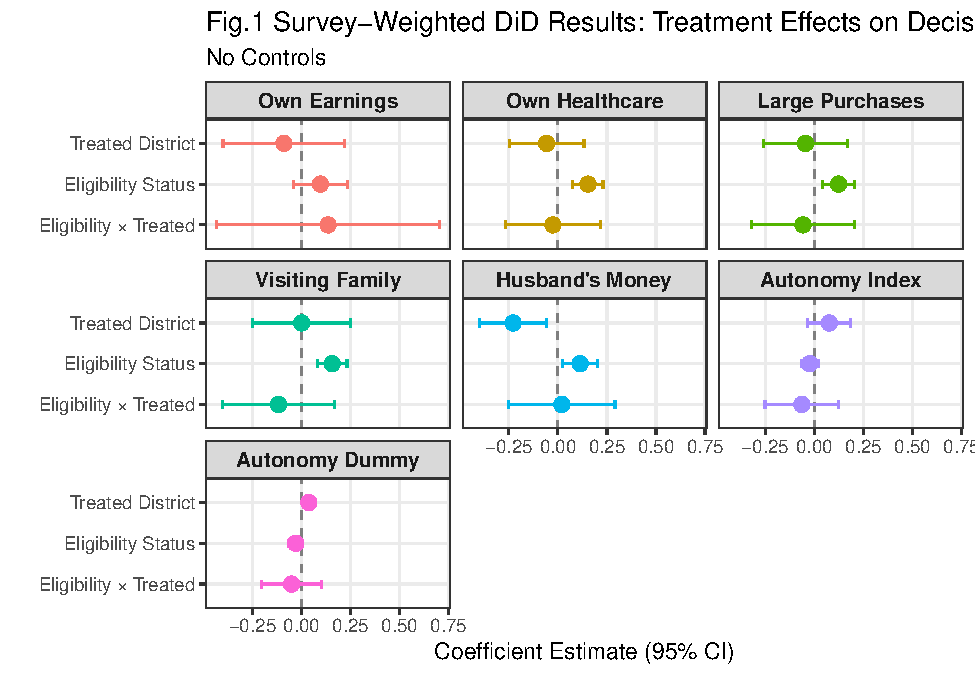
\includegraphics[keepaspectratio]{Results-3_files/figure-latex/Regression Graphs-1.pdf}}
\pandocbounded{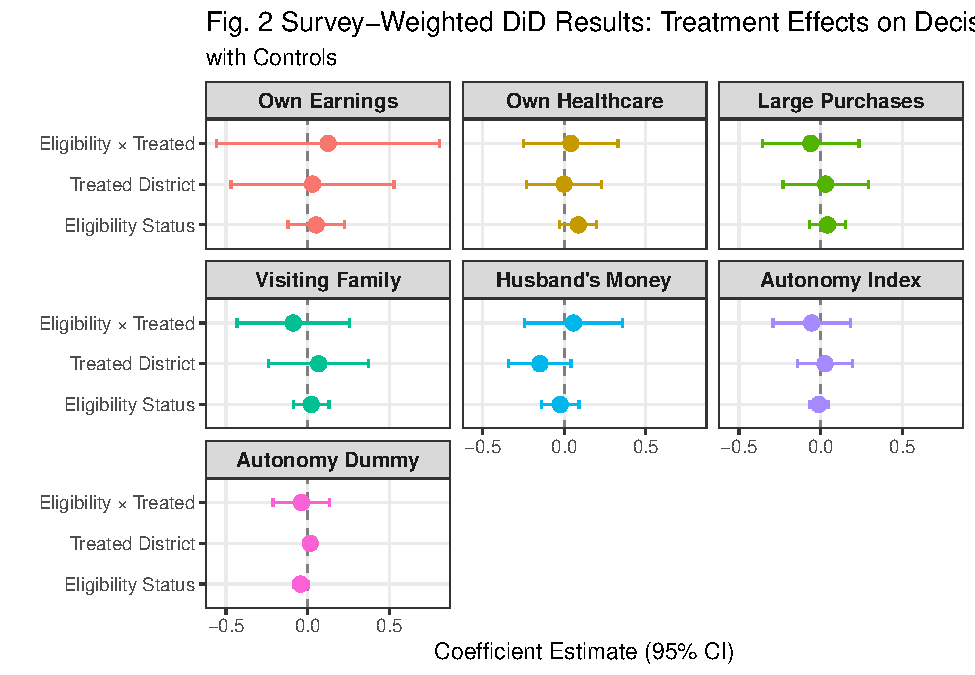
\includegraphics[keepaspectratio]{Results-3_files/figure-latex/Regression Graphs-2.pdf}}
\pandocbounded{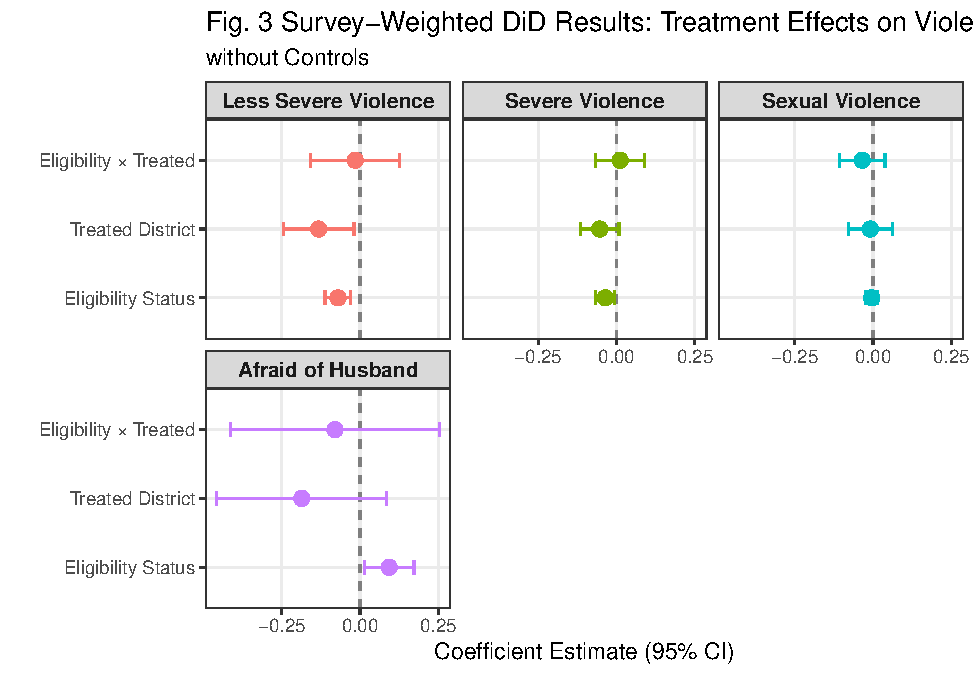
\includegraphics[keepaspectratio]{Results-3_files/figure-latex/Regression Graphs-3.pdf}}
\pandocbounded{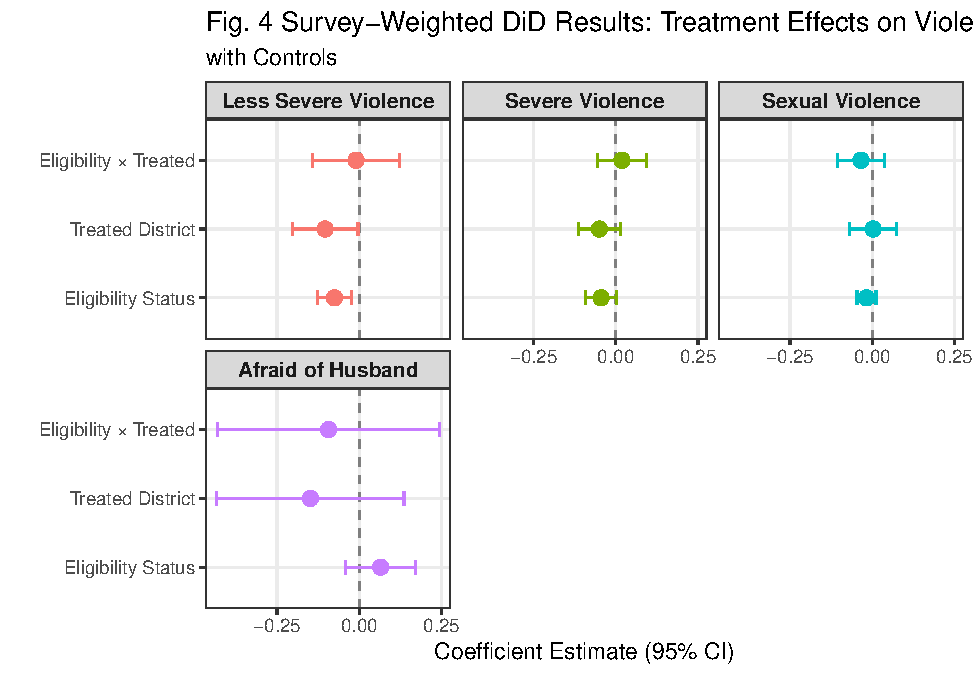
\includegraphics[keepaspectratio]{Results-3_files/figure-latex/Regression Graphs-4.pdf}}
\pandocbounded{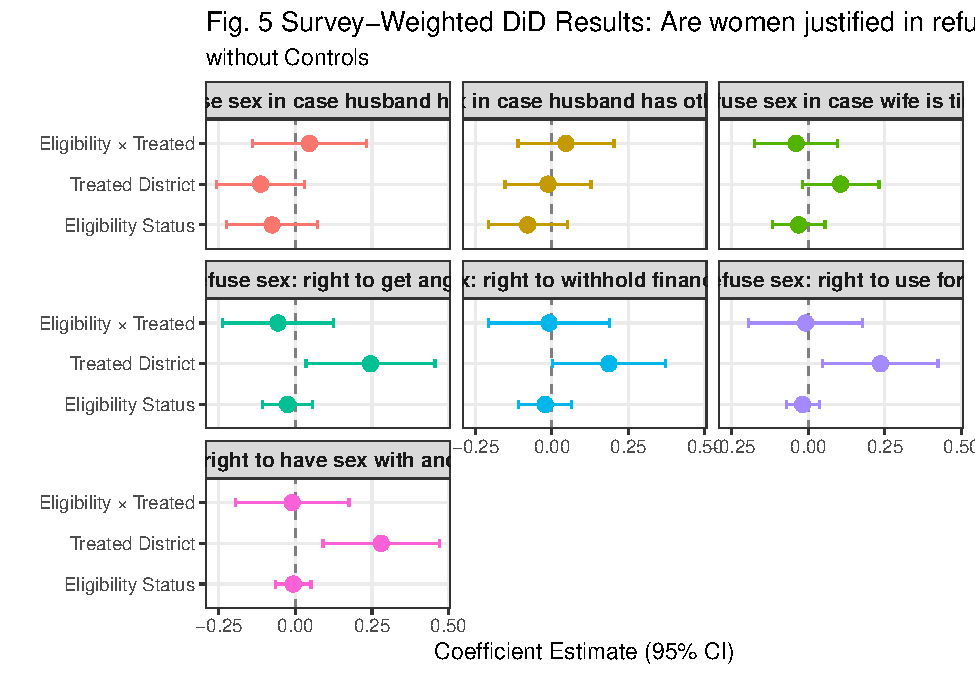
\includegraphics[keepaspectratio]{Results-3_files/figure-latex/Regression Graphs-5.pdf}}
\pandocbounded{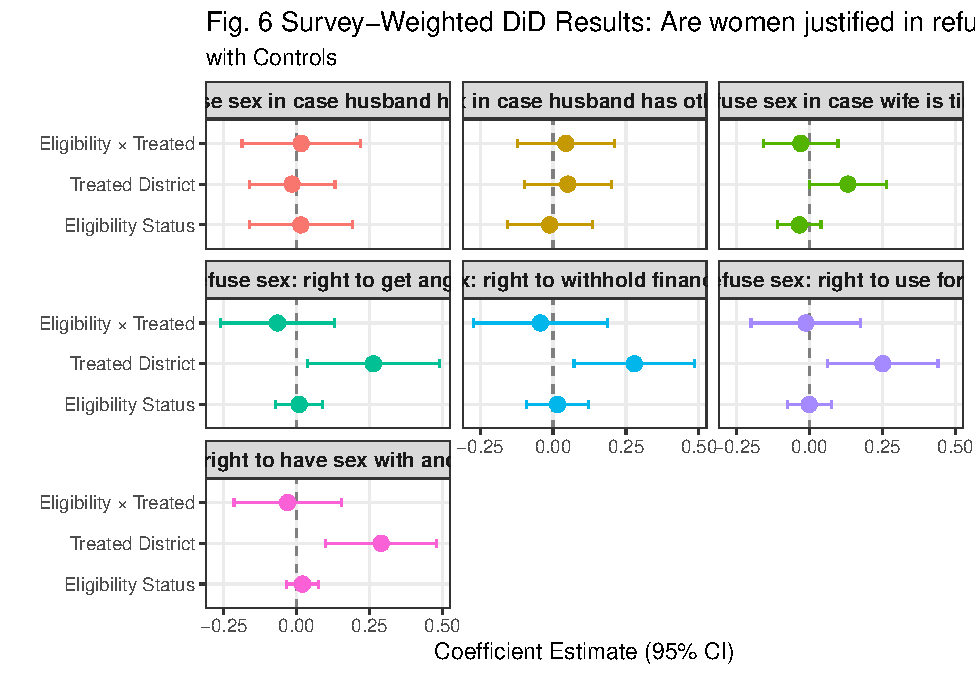
\includegraphics[keepaspectratio]{Results-3_files/figure-latex/Regression Graphs-6.pdf}}
\pandocbounded{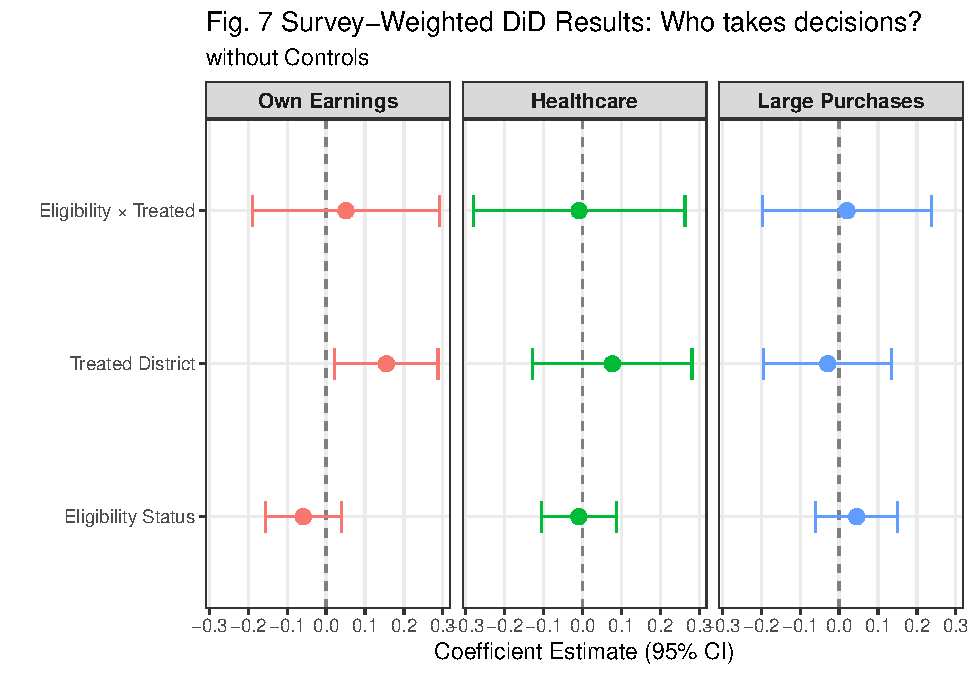
\includegraphics[keepaspectratio]{Results-3_files/figure-latex/Regression Graphs-7.pdf}}
\pandocbounded{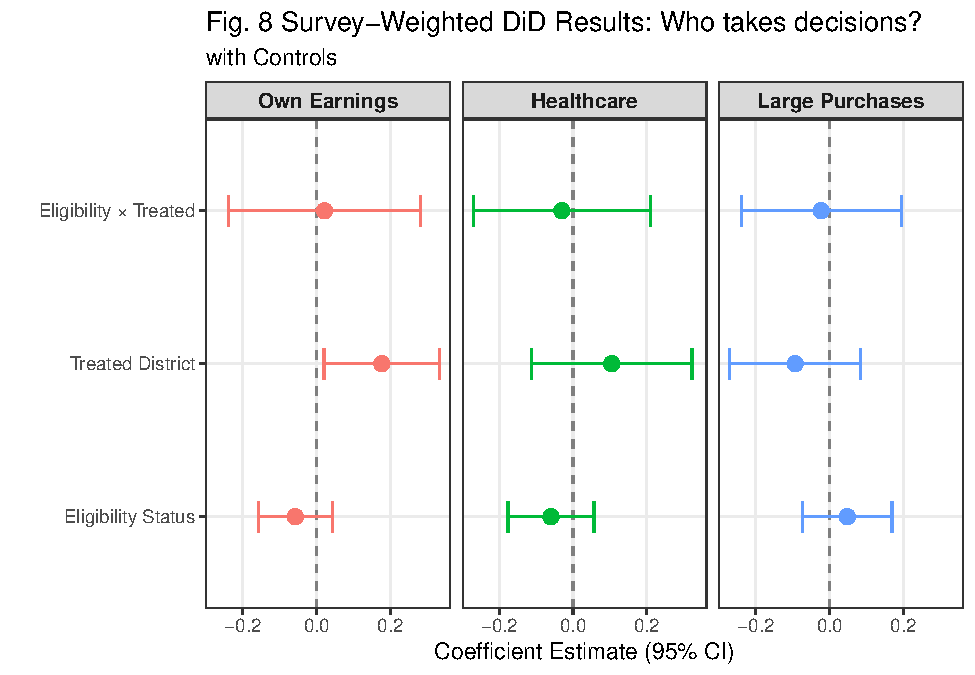
\includegraphics[keepaspectratio]{Results-3_files/figure-latex/Regression Graphs-8.pdf}}
\pandocbounded{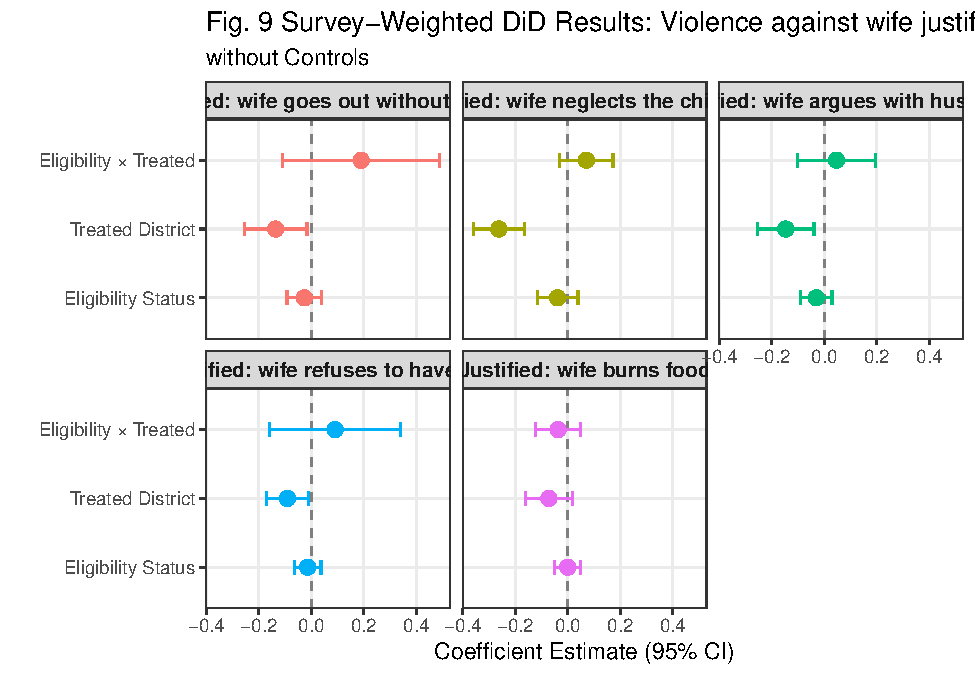
\includegraphics[keepaspectratio]{Results-3_files/figure-latex/Regression Graphs-9.pdf}}
\pandocbounded{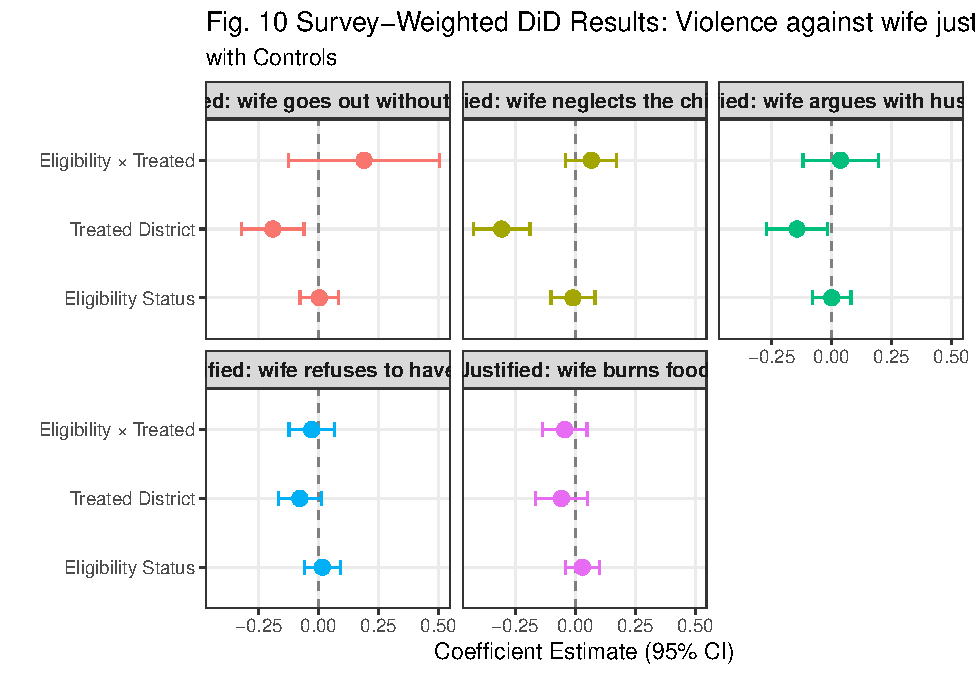
\includegraphics[keepaspectratio]{Results-3_files/figure-latex/Regression Graphs-10.pdf}}
\pandocbounded{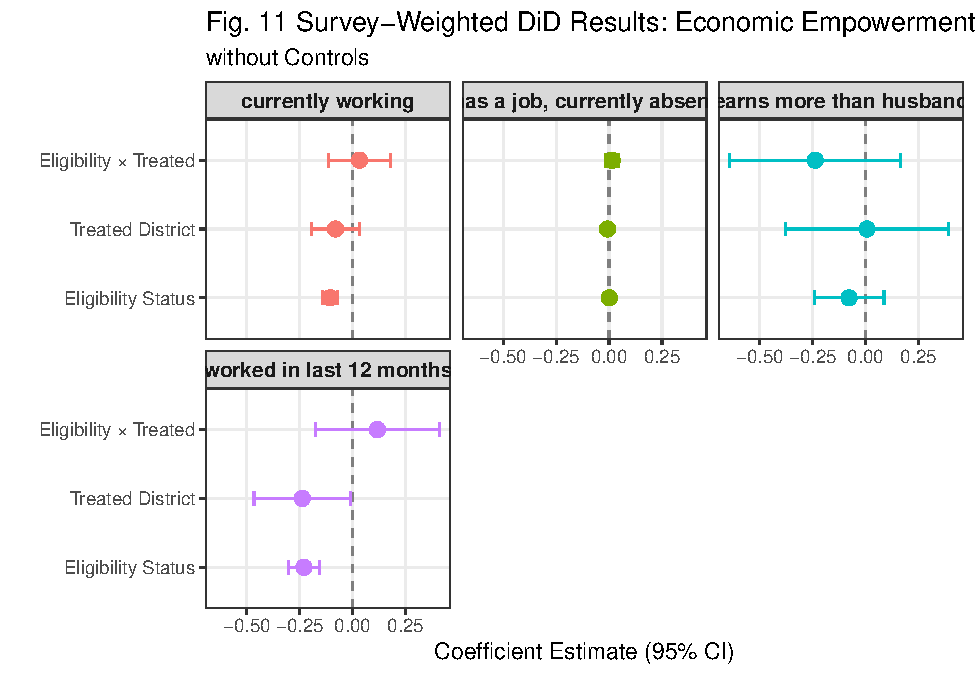
\includegraphics[keepaspectratio]{Results-3_files/figure-latex/Regression Graphs-11.pdf}}
\pandocbounded{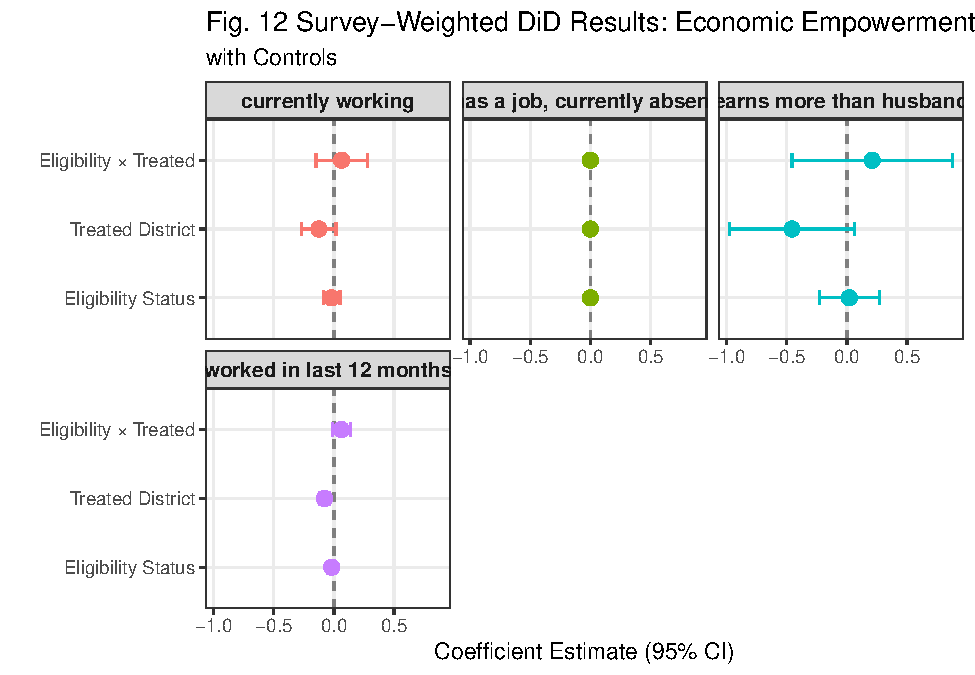
\includegraphics[keepaspectratio]{Results-3_files/figure-latex/Regression Graphs-12.pdf}}

\end{document}
